% =============================================================================
% Laporan Kerja Praktik — Platform Asesmen Psikologi Digital CHP
% Sanders · 412023020 · Informatika · FTC · UKRIDA · 2025
% =============================================================================
\documentclass[12pt,a4paper,oneside]{report}

% ── Encoding ──────────────────────────────────────────────────────────────────
\usepackage[utf8]{inputenc}
\usepackage[T1]{fontenc}
\usepackage{amsmath}

% ── Font: Times New Roman ─────────────────────────────────────────────────────
\usepackage{mathptmx}

% ── Page Layout (Pedoman: L=4cm, R=3cm, T=3cm, B=3cm) ────────────────────────
\usepackage[left=4cm, right=3cm, top=3cm, bottom=3cm]{geometry}

% ── Spacing: Spasi Dua (double spacing) ───────────────────────────────────────
\usepackage{setspace}
\setstretch{2}
\emergencystretch=3em
\raggedbottom
\hbadness=10001
\vbadness=10001
\hfuzz=2pt
\AtBeginDocument{%
  \hbadness=10001%
  \vbadness=10001%
  \hfuzz=2pt%
}
\makeatletter
\g@addto@macro\@arrayparboxrestore{%
  \hbadness=10001%
  \vbadness=10001%
  \hfuzz=2pt%
}
\makeatother

% ── Chapter & Section Titles ──────────────────────────────────────────────────
\usepackage{titlesec}

% BAB heading: 14pt bold centered uppercase
\titleformat{\chapter}[display]
  {\normalfont\fontsize{14}{16}\bfseries\centering}
  {\MakeUppercase{\chaptertitlename}\ \thechapter}{0pt}
  {\fontsize{14}{16}\bfseries\MakeUppercase}
\titlespacing*{\chapter}{0pt}{-20pt}{20pt}

% Section heading: 12pt bold
\titleformat{\section}
  {\normalfont\fontsize{12}{14}\bfseries}
  {\thesection}{1em}{}

% Subsection heading: 12pt bold
\titleformat{\subsection}
  {\normalfont\fontsize{12}{14}\bfseries}
  {\thesubsection}{1em}{}

% Subsubsection heading: 12pt bold
\titleformat{\subsubsection}
  {\normalfont\fontsize{12}{14}\bfseries}
  {\thesubsubsection}{1em}{}

% ── Page Numbering & Headers ──────────────────────────────────────────────────
\usepackage{fancyhdr}

% Default style for body: Arabic, bottom-right
\fancypagestyle{body}{%
  \fancyhf{}%
  \fancyfoot[R]{\thepage}%
  \renewcommand{\headrulewidth}{0pt}%
}

% Style for front matter: Roman, bottom-right
\fancypagestyle{frontmatter}{%
  \fancyhf{}%
  \fancyfoot[R]{\thepage}%
  \renewcommand{\headrulewidth}{0pt}%
}

% Style for chapter opening pages
\fancypagestyle{plain}{%
  \fancyhf{}%
  \fancyfoot[R]{\thepage}%
  \renewcommand{\headrulewidth}{0pt}%
}

% ── Tables ────────────────────────────────────────────────────────────────────
\usepackage{booktabs}
\usepackage{longtable}
\usepackage{tabularx}
\usepackage{xltabular}
\usepackage{array}
\usepackage{multirow}

% -- Microtypography & long-token breaking --
\usepackage{microtype}
\usepackage{seqsplit}

% ── Graphics ──────────────────────────────────────────────────────────────────
\usepackage{graphicx}
\usepackage{float}
\usepackage{svg}
\usepackage{pdfpages}
\graphicspath{{figures/}}
\svgpath{{figures/}}

% ── Algorithm ─────────────────────────────────────────────────────────────────
\usepackage{algorithm}
\usepackage{algorithmic}

% ── Lists ─────────────────────────────────────────────────────────────────────
\usepackage{enumitem}

% ── Caption formatting ────────────────────────────────────────────────────────
\usepackage{caption}
\captionsetup{font={small}, labelfont={bf}, skip=8pt}

% ── Custom Commands ───────────────────────────────────────────────────────────
\newcommand{\judulLaporan}{Perancangan dan Pengembangan Platform Asesmen Psikologi Digital untuk Pusat Kesehatan Psikologi (CHP) Universitas Kristen Krida Wacana}
\newcommand{\namaMahasiswa}{Sanders Keane Dylan Daniyolla}
\newcommand{\nimMahasiswa}{412023020}
\newcommand{\prodiMahasiswa}{Informatika}
\newcommand{\fakultasMahasiswa}{Fakultas Teknologi Cerdas (FTC)}
\newcommand{\universitasMahasiswa}{Universitas Kristen Krida Wacana}
\newcommand{\tahunSidang}{2026}

% ── Indonesian babel (optional, for hyphenation) ──────────────────────────────
\usepackage[indonesian]{babel}
\addto\captionsindonesian{\renewcommand{\bibname}{DAFTAR PUSTAKA}}

% ── Hyperlinks (load last) ────────────────────────────────────────────────────
\usepackage[hidelinks,hypertexnames=false]{hyperref}

% =============================================================================
% DOCUMENT
% =============================================================================
\begin{document}

% ═══════════════════════════════════════════════════════════════════════════════
% FRONT MATTER — Roman numerals, bottom-right
% ═══════════════════════════════════════════════════════════════════════════════
\pagenumbering{roman}
\pagestyle{frontmatter}

% ── Halaman Judul (counted but NOT printed) ───────────────────────────────────
% =============================================================================
% 00-title.tex — Halaman Judul (Lembar Cover dari Template Universitas)
% =============================================================================
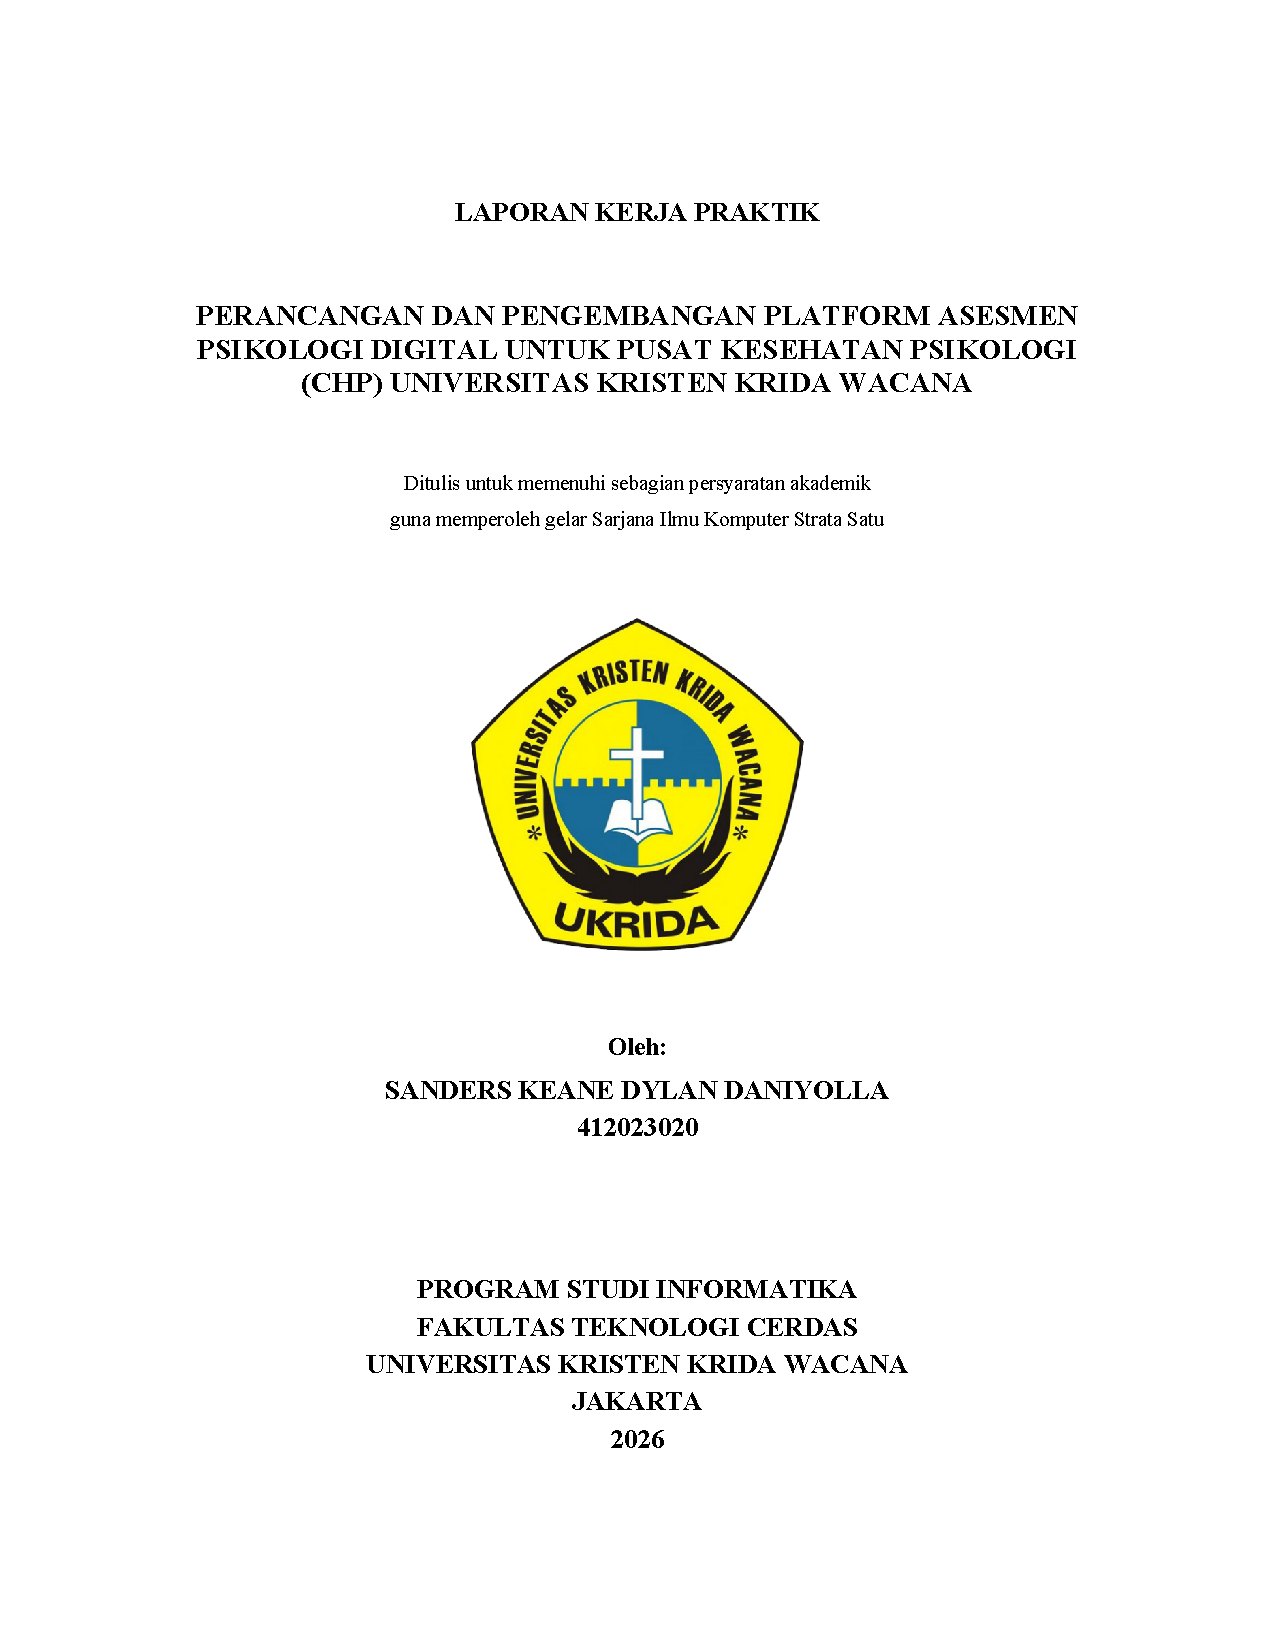
\includepdf[pages=-,pagecommand={\thispagestyle{empty}}]{parts/00-cover.pdf}


% ── Halaman Persetujuan (counted but NOT printed) ─────────────────────────────
% =============================================================================
% 01-persetujuan.tex — Halaman Persetujuan (Lembar Persetujuan dari Template Universitas)
% =============================================================================
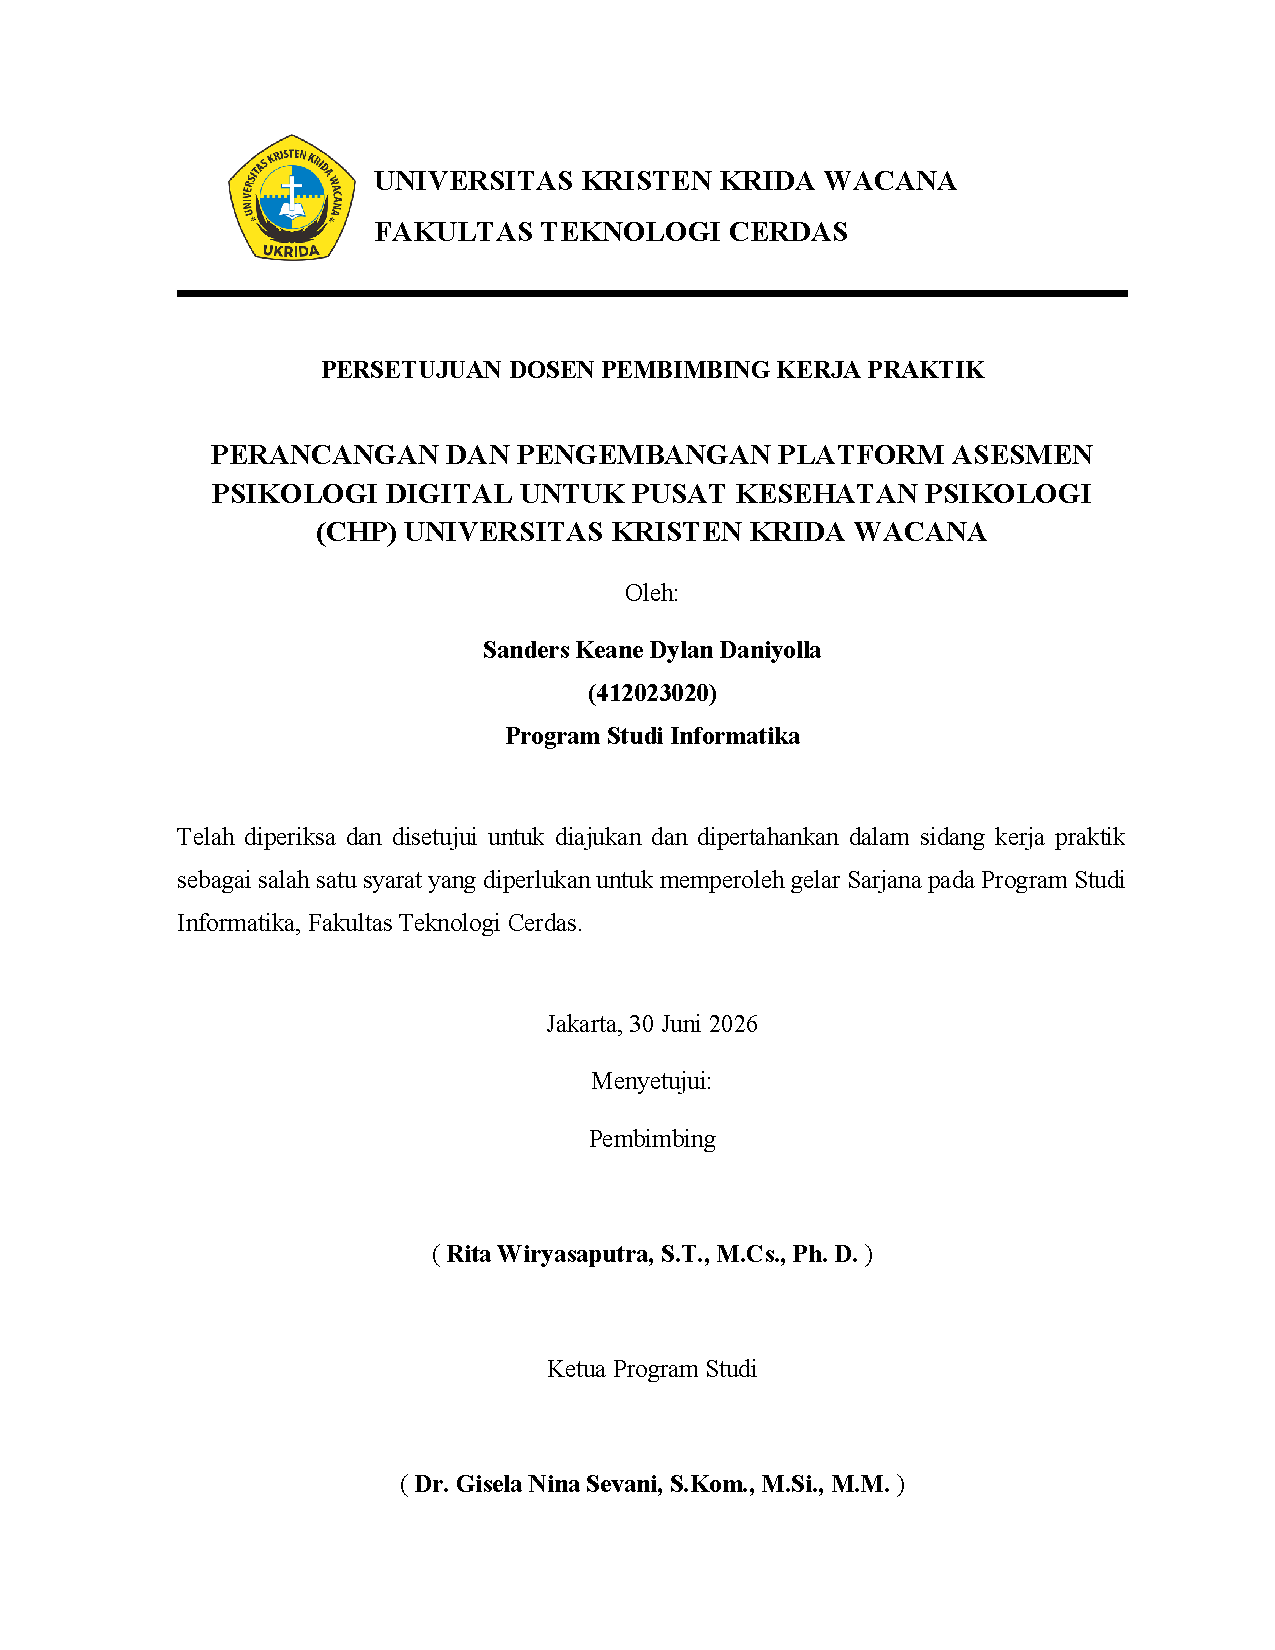
\includepdf[pages=-,pagecommand={\thispagestyle{empty}}]{parts/01-persetujuan.pdf}


% ── Halaman Pengesahan (counted but NOT printed) ──────────────────────────────
% =============================================================================
% 02-pengesahan.tex — Halaman Pengesahan
% =============================================================================
\clearpage
\thispagestyle{empty}

\begin{singlespace}
\begin{center}
  {\fontsize{14}{16}\selectfont\bfseries HALAMAN PENGESAHAN}\\[0.5cm]
  {\fontsize{14}{16}\selectfont\bfseries LAPORAN KERJA PRAKTIK}\\[1.5cm]
  {\fontsize{12}{14}\selectfont\bfseries \judulLaporan}\\[1cm]
\end{center}

\noindent Laporan Kerja Praktik ini telah dipertahankan di hadapan tim penguji pada:

\vspace{0.5cm}
\noindent
\begin{tabular}{@{}ll@{}}
  Hari/Tanggal & : \rule{6cm}{0.4pt} \\[0.3cm]
  Tempat & : Program Studi Informatika, FTC, UKRIDA \\
\end{tabular}

\vspace{1cm}

\noindent dan dinyatakan \textbf{LULUS} dengan nilai \rule{3cm}{0.4pt}.

\vspace{1.5cm}

\begin{center}
  {\bfseries Tim Penguji}
\end{center}

\vspace{0.5cm}

\noindent
\begin{minipage}[t]{0.48\textwidth}
  \begin{center}
    Penguji I,\\[2.5cm]
    \rule{5cm}{0.4pt}\\
    NIP.
  \end{center}
\end{minipage}
\hfill
\begin{minipage}[t]{0.48\textwidth}
  \begin{center}
    Penguji II,\\[2.5cm]
    \rule{5cm}{0.4pt}\\
    NIP.
  \end{center}
\end{minipage}

\vspace{1cm}

\begin{center}
  Mengetahui,\\
  Ketua Program Studi Informatika\\[2.5cm]
  \rule{6cm}{0.4pt}\\
  NIP.
\end{center}

\end{singlespace}


% ── Kata Pengantar (first printed Roman numeral) ──────────────────────────────
% =============================================================================
% 03-kata-pengantar.tex — Kata Pengantar
% =============================================================================
\clearpage
\phantomsection
\addcontentsline{toc}{chapter}{KATA PENGANTAR}

\begin{center}
  {\fontsize{14}{16}\selectfont\bfseries KATA PENGANTAR}
\end{center}

\vspace{1cm}

Puji dan syukur penulis panjatkan kepada Tuhan Yang Maha Esa atas berkat dan rahmat-Nya sehingga penulis dapat menyelesaikan laporan Kerja Praktik yang berjudul ``\judulLaporan'' dengan baik dan tepat waktu.

Laporan ini disusun sebagai salah satu syarat untuk menyelesaikan mata kuliah Kerja Praktik pada Program Studi Informatika, Fakultas Teknologi Cerdas, Universitas Kristen Krida Wacana. Kerja Praktik ini dilaksanakan menggunakan skema Proyek Dosen di bawah bimbingan langsung Ibu Astin selaku Ketua Program Studi Psikologi dan Kepala Riset \textit{Center for Health Psychology} (CHP) UKRIDA.

Penulis menyadari bahwa laporan ini tidak dapat diselesaikan tanpa bantuan dan dukungan dari berbagai pihak. Oleh karena itu, penulis ingin menyampaikan ucapan terima kasih yang sebesar-besarnya kepada:

\begin{enumerate}[leftmargin=2cm]
  \item Ibu Astin selaku pemilik proyek dan Kepala Riset CHP UKRIDA, yang telah memberikan kesempatan, arahan, dan umpan balik yang berharga selama pelaksanaan Kerja Praktik.
  \item Dosen Pembimbing Kerja Praktik yang telah membimbing penulis dalam penyusunan laporan ini.
  \item Seluruh dosen dan staf Program Studi Informatika, FTC, UKRIDA yang telah memberikan bekal ilmu dan dukungan selama perkuliahan.
  \item Rekan satu tim yang telah berkolaborasi dalam pengembangan Platform Asesmen Digital CHP.
  \item Keluarga tercinta yang senantiasa memberikan doa, motivasi, dan dukungan moral selama proses pelaksanaan Kerja Praktik.
\end{enumerate}

Penulis menyadari bahwa laporan ini masih jauh dari kesempurnaan. Oleh karena itu, penulis mengharapkan kritik dan saran yang membangun demi perbaikan di masa mendatang. Semoga laporan ini dapat memberikan manfaat bagi pembaca dan menjadi kontribusi yang berarti bagi pengembangan platform asesmen psikologi digital di Indonesia.

\vspace{2cm}

\noindent
\begin{flushright}
  Jakarta, 30 Juni \tahunSidang\\[1.5cm]
  \namaMahasiswa
\end{flushright}


% ── Daftar Isi ────────────────────────────────────────────────────────────────
% =============================================================================
% 04-daftar-isi.tex — Daftar Isi (Auto-generated)
% =============================================================================
\clearpage
\phantomsection
\addcontentsline{toc}{chapter}{DAFTAR ISI}
\begin{singlespace}
\tableofcontents

\end{singlespace}

% ── Daftar Tabel ──────────────────────────────────────────────────────────────
% =============================================================================
% 05-daftar-tabel.tex — Daftar Tabel (Auto-generated)
% =============================================================================
\clearpage
\phantomsection
\addcontentsline{toc}{chapter}{DAFTAR TABEL}
\listoftables


% ── Daftar Gambar ─────────────────────────────────────────────────────────────
% =============================================================================
% 06-daftar-gambar.tex — Daftar Gambar (Auto-generated)
% =============================================================================
\clearpage
\phantomsection
\addcontentsline{toc}{chapter}{DAFTAR GAMBAR}
\listoffigures


% ═══════════════════════════════════════════════════════════════════════════════
% BODY — Arabic numerals, bottom-right
% BAB numbering: I → II → III → IV → V (sequential)
% ═══════════════════════════════════════════════════════════════════════════════
\clearpage
\pagenumbering{arabic}
\pagestyle{body}

% ── BAB I: Pendahuluan ──────────────────────────────────────────────────────
% =============================================================================
% 10-bab1.tex — BAB I PENDAHULUAN
% Patches applied: F1 (remove placeholder), F2 (update goals), C1 (20 tabel)
% =============================================================================
\chapter{PENDAHULUAN}
\label{chap:pendahuluan}

% ─────────────────────────────────────────────────────────────────────────────
\section{Latar Belakang}
\label{sec:latar-belakang}

\textit{Center for Health Psychology} (CHP) adalah unit riset di bawah Program Studi Psikologi, Universitas Kristen Krida Wacana (UKRIDA), yang berperan sebagai pusat rujukan dalam bidang kesehatan mental dan penelitian psikologi klinis. Untuk menjalankan misi tersebut, CHP membutuhkan platform digital yang kokoh, bukan sekadar situs kuis daring, melainkan sebuah instrumen penelitian digital yang harus memenuhi standar validitas dan reliabilitas psikometrik. Prinsip fundamental ini menjadi landasan seluruh keputusan perancangan dalam proyek Kerja Praktik (KP) ini.

% --- Professor-approved: Three manual methods ---
Sebelum proyek ini dimulai, CHP menggunakan tiga metode manual untuk melaksanakan asesmen psikologi. \textbf{Pertama}, metode \textit{paper-based}: responden mengisi lembar jawaban secara manual dan administrator menghitung skor menggunakan panduan penilaian (\textit{scoring guide}) masing-masing instrumen. \textbf{Kedua}, metode \textit{spreadsheet} Excel: administrator mewawancarai responden dan memasukkan data ke dalam lembar kerja Excel; beberapa instrumen telah memiliki rumus otomatis, namun pengelolaan data secara keseluruhan tetap bersifat manual. \textbf{Ketiga}, metode Google Forms: pengumpulan jawaban dilakukan secara daring, namun data harus diekspor terlebih dahulu dan diproses secara manual di luar sistem. Tidak satu pun dari ketiga metode tersebut mampu menyimpan, mengarsipkan, dan memproses data asesmen secara terintegrasi dan otomatis.

% --- Professor-approved: Four operational problems ---
Kondisi ini menimbulkan empat masalah operasional utama:

\begin{enumerate}[leftmargin=2cm]
  \item Proses penilaian yang lambat dan rentan terhadap kesalahan manusia (\textit{human error}), terutama pada instrumen dengan banyak butir soal dan subskala.
  \item Data asesmen tidak tersimpan secara terpusat dan terstruktur, sehingga sulit diakses untuk keperluan penelitian longitudinal.
  \item Tidak tersedia fitur ekspor data berkualitas riset yang kompatibel dengan perangkat lunak analisis statistik seperti SPSS atau JASP.
  \item Asesmen jarak jauh (\textit{remote assessment}) tidak dapat dilaksanakan secara efektif karena ketergantungan pada proses manual.
\end{enumerate}

% --- Professor-approved: Platform capabilities ---
Platform yang dikembangkan dalam proyek KP ini dirancang untuk mengakomodasi seluruh alur kerja asesmen. Responden dapat mengisi asesmen secara daring (\textit{online}) maupun di lokasi (\textit{on-site}). Administrator dapat mengimpor data asesmen manual---baik dari lembar \textit{paper-based} maupun Excel---ke dalam sistem. Seluruh komputasi skor dilakukan secara instan oleh \textit{scoring engine} tanpa intervensi manual. Metode tradisional (\textit{paper-based} atau Excel di lokasi terpencil) tetap dapat digunakan, dan hasilnya dapat diintegrasikan ke dalam platform ketika koneksi tersedia.

Platform ini terdiri atas beberapa modul terintegrasi: modul asesmen yang mengelola siklus hidup pengerjaan tes mulai dari persetujuan peserta hingga komputasi skor; modul administrasi yang menyediakan antarmuka bagi tim psikologi untuk mengelola instrumen, memantau statistik, dan mengekspor data riset; modul autentikasi yang mengimplementasikan sistem keamanan berlapis; serta modul pelaporan yang menghasilkan dokumen hasil asesmen dan mengirimkannya melalui surel.

% --- Professor-approved: Four instrument descriptions ---
Pada tahap awal, platform mengimplementasikan empat instrumen psikometri yang diprioritaskan oleh tim peneliti CHP:

\textbf{\textit{Generalized Problematic Internet Use Scale} 2 (GPIUS-2)} adalah instrumen yang mengukur penggunaan internet bermasalah berdasarkan model kognitif-perilaku. GPIUS-2 terdiri atas 15 butir soal yang terbagi ke dalam lima subskala: \textit{Preference for Online Social Interaction} (POSI), regulasi suasana hati (\textit{mood regulation}), preokupasi kognitif (\textit{cognitive preoccupation}), penggunaan kompulsif (\textit{compulsive use}), dan dampak negatif (\textit{negative outcomes}). Instrumen ini menggunakan skala Likert delapan poin (1--8) dengan rentang skor total 15--120. Rincian butir soal terdapat pada Lampiran~1. Catatan: platform mengimplementasikan versi adaptasi dengan skala Likert 1--5 sesuai keputusan tim peneliti CHP.

\textbf{\textit{Perceived Stress Scale} 10 (PSS-10)} adalah instrumen yang dikembangkan oleh Cohen, Kamarck, dan Mermelstein (1983) untuk mengukur persepsi stres individu \cite{cohen1983}. PSS-10 terdiri atas 10 butir soal yang terbagi ke dalam dua subskala: \textit{perceived helplessness} (6 butir soal) dan \textit{perceived self-efficacy} (4 butir soal terbalik). Instrumen ini menggunakan skala Likert lima poin (0--4) dengan rentang skor total 0--40. PSS-10 telah divalidasi untuk responden berusia 12 tahun ke atas dan telah diterjemahkan ke dalam lebih dari 25 bahasa. Rincian butir soal terdapat pada Lampiran~2.

\textbf{\textit{Self-Reporting Questionnaire} 29 (SRQ-29)} adalah instrumen skrining yang dikembangkan oleh \textit{World Health Organization} (WHO) untuk mendeteksi gangguan kesehatan mental umum. SRQ-29 terdiri atas 29 butir soal dengan format jawaban biner (Ya/Tidak) yang terbagi ke dalam empat domain: somatik, kecemasan, depresi, dan psikosis. Rincian butir soal terdapat pada Lampiran~3.

\textbf{\textit{Stress Response Scale} (SRS)} adalah instrumen yang mengukur kapasitas respons stres individu. SRS terdiri atas 29 butir soal yang terbagi ke dalam tiga dimensi: \textit{self-efficacy}, kepuasan (\textit{satisfaction}), dan kontrol yang dipersepsikan (\textit{perceived control}). Skor yang lebih tinggi mengindikasikan kapasitas regulasi diri yang lebih besar. Rincian butir soal terdapat pada Lampiran~4.

Evaluasi teknis mendalam terhadap sistem web CHP yang sebelumnya dikembangkan oleh tim mahasiswa mengungkapkan sejumlah defisiensi fundamental. Sistem lama dibangun menggunakan \textit{HyperText Markup Language} (HTML), \textit{Cascading Style Sheets} (CSS), dan JavaScript (JS) murni tanpa \textit{framework} apapun, sehingga tidak memiliki struktur arsitektur yang memadai untuk kebutuhan riset jangka panjang. \textit{Technical debt} (akumulasi dampak negatif dari keputusan desain yang tidak optimal) pada sistem lama bersifat struktural, bukan superfisial. Akibatnya, upaya perbaikan tambal sulam akan memakan lebih banyak sumber daya dibandingkan pembangunan ulang dari nol, namun tetap menghasilkan produk yang inferior. Tabel~\ref{tab:defisiensi} merangkum seluruh defisiensi yang ditemukan beserta dampak operasionalnya.

\begin{table}[htbp]
  \centering
  \caption{Defisiensi Sistem CHP Terdahulu}
  \label{tab:defisiensi}
  \begin{tabularx}{\textwidth}{@{}l X X@{}}
    \toprule
    \textbf{Masalah} & \textbf{Deskripsi} & \textbf{Dampak} \\
    \midrule
    Tanpa \textit{Framework} & HTML/CSS/JS murni tanpa struktur arsitektur & Tidak dapat di-\textit{scale}, dipelihara, atau diuji secara sistematis \\
    Struktur File Datar & Semua \textit{file} di direktori root tanpa pemisahan \textit{concerns} & Setiap modifikasi berisiko menyebabkan kegagalan berantai di bagian lain \\
    Tanpa \textit{Type Safety} & JavaScript biasa tanpa \textit{type checking} atau \textit{linting} & \textit{Bug} tersembunyi mencapai produksi tanpa terdeteksi \\
    Cakupan Tes Nol & Tidak ada \textit{unit test}, \textit{integration test}, maupun \textit{end-to-end test} & \textit{Bug} regresi tidak terelakkan pada setiap perubahan kode \\
    Desain Basis Data Tidak Memadai & Skema tidak dapat memodelkan penilaian multidimensional bervariasi & Memblokir fungsionalitas riset inti \\
    Tanpa Dokumentasi & Tidak ada README, dokumentasi API, atau panduan \textit{setup} & Setiap kontributor baru memulai dari nol tanpa acuan \\
    \bottomrule
  \end{tabularx}
\end{table}

Berdasarkan temuan pada Tabel~\ref{tab:defisiensi}, solusi yang dipilih adalah pembangunan ulang total (\textit{full redevelopment}) menggunakan \textit{tech stack} modern berstandar industri. Platform baru dibangun di atas Next.js 16 sebagai \textit{meta-framework} berbasis React, TypeScript sebagai bahasa pemrograman utama yang memberikan keamanan tipe (\textit{type safety}), PostgreSQL sebagai Sistem Manajemen Basis Data Relasional (\textit{Relational Database Management System}/RDBMS), tRPC untuk lapisan API yang aman secara tipe dari ujung ke ujung (\textit{end-to-end type safety}), serta Drizzle \textit{Object-Relational Mapping} (ORM) sebagai lapisan abstraksi basis data. Seluruh sistem di-\textit{deploy} pada platform \textit{serverless} Vercel dengan basis data terkelola melalui Neon PostgreSQL dan \textit{caching} melalui Upstash Redis.

% --- Professor-approved: Updated user groups (3 groups) ---
Sistem yang dibangun melayani tiga kelompok pengguna utama: (1) masyarakat umum termasuk mahasiswa yang membutuhkan asesmen kesehatan mental mandiri (\textit{self-assessment}); (2) administrator dan tim riset psikologi yang mengelola instrumen, memantau sesi, dan mengekspor data berkualitas riset; serta (3) super administrator yang mengelola seluruh akun admin dalam sistem. Metodologi pengembangan yang digunakan adalah Agile iteratif dengan siklus \textit{sprint} dua mingguan, memungkinkan umpan balik berkelanjutan dari pemangku kepentingan di setiap tahap pengembangan. Gambar~\ref{fig:arsitektur-umum} menampilkan gambaran umum arsitektur sistem platform CHP yang dirancang dalam proyek ini.

\begin{figure}[htbp]
  \centering
  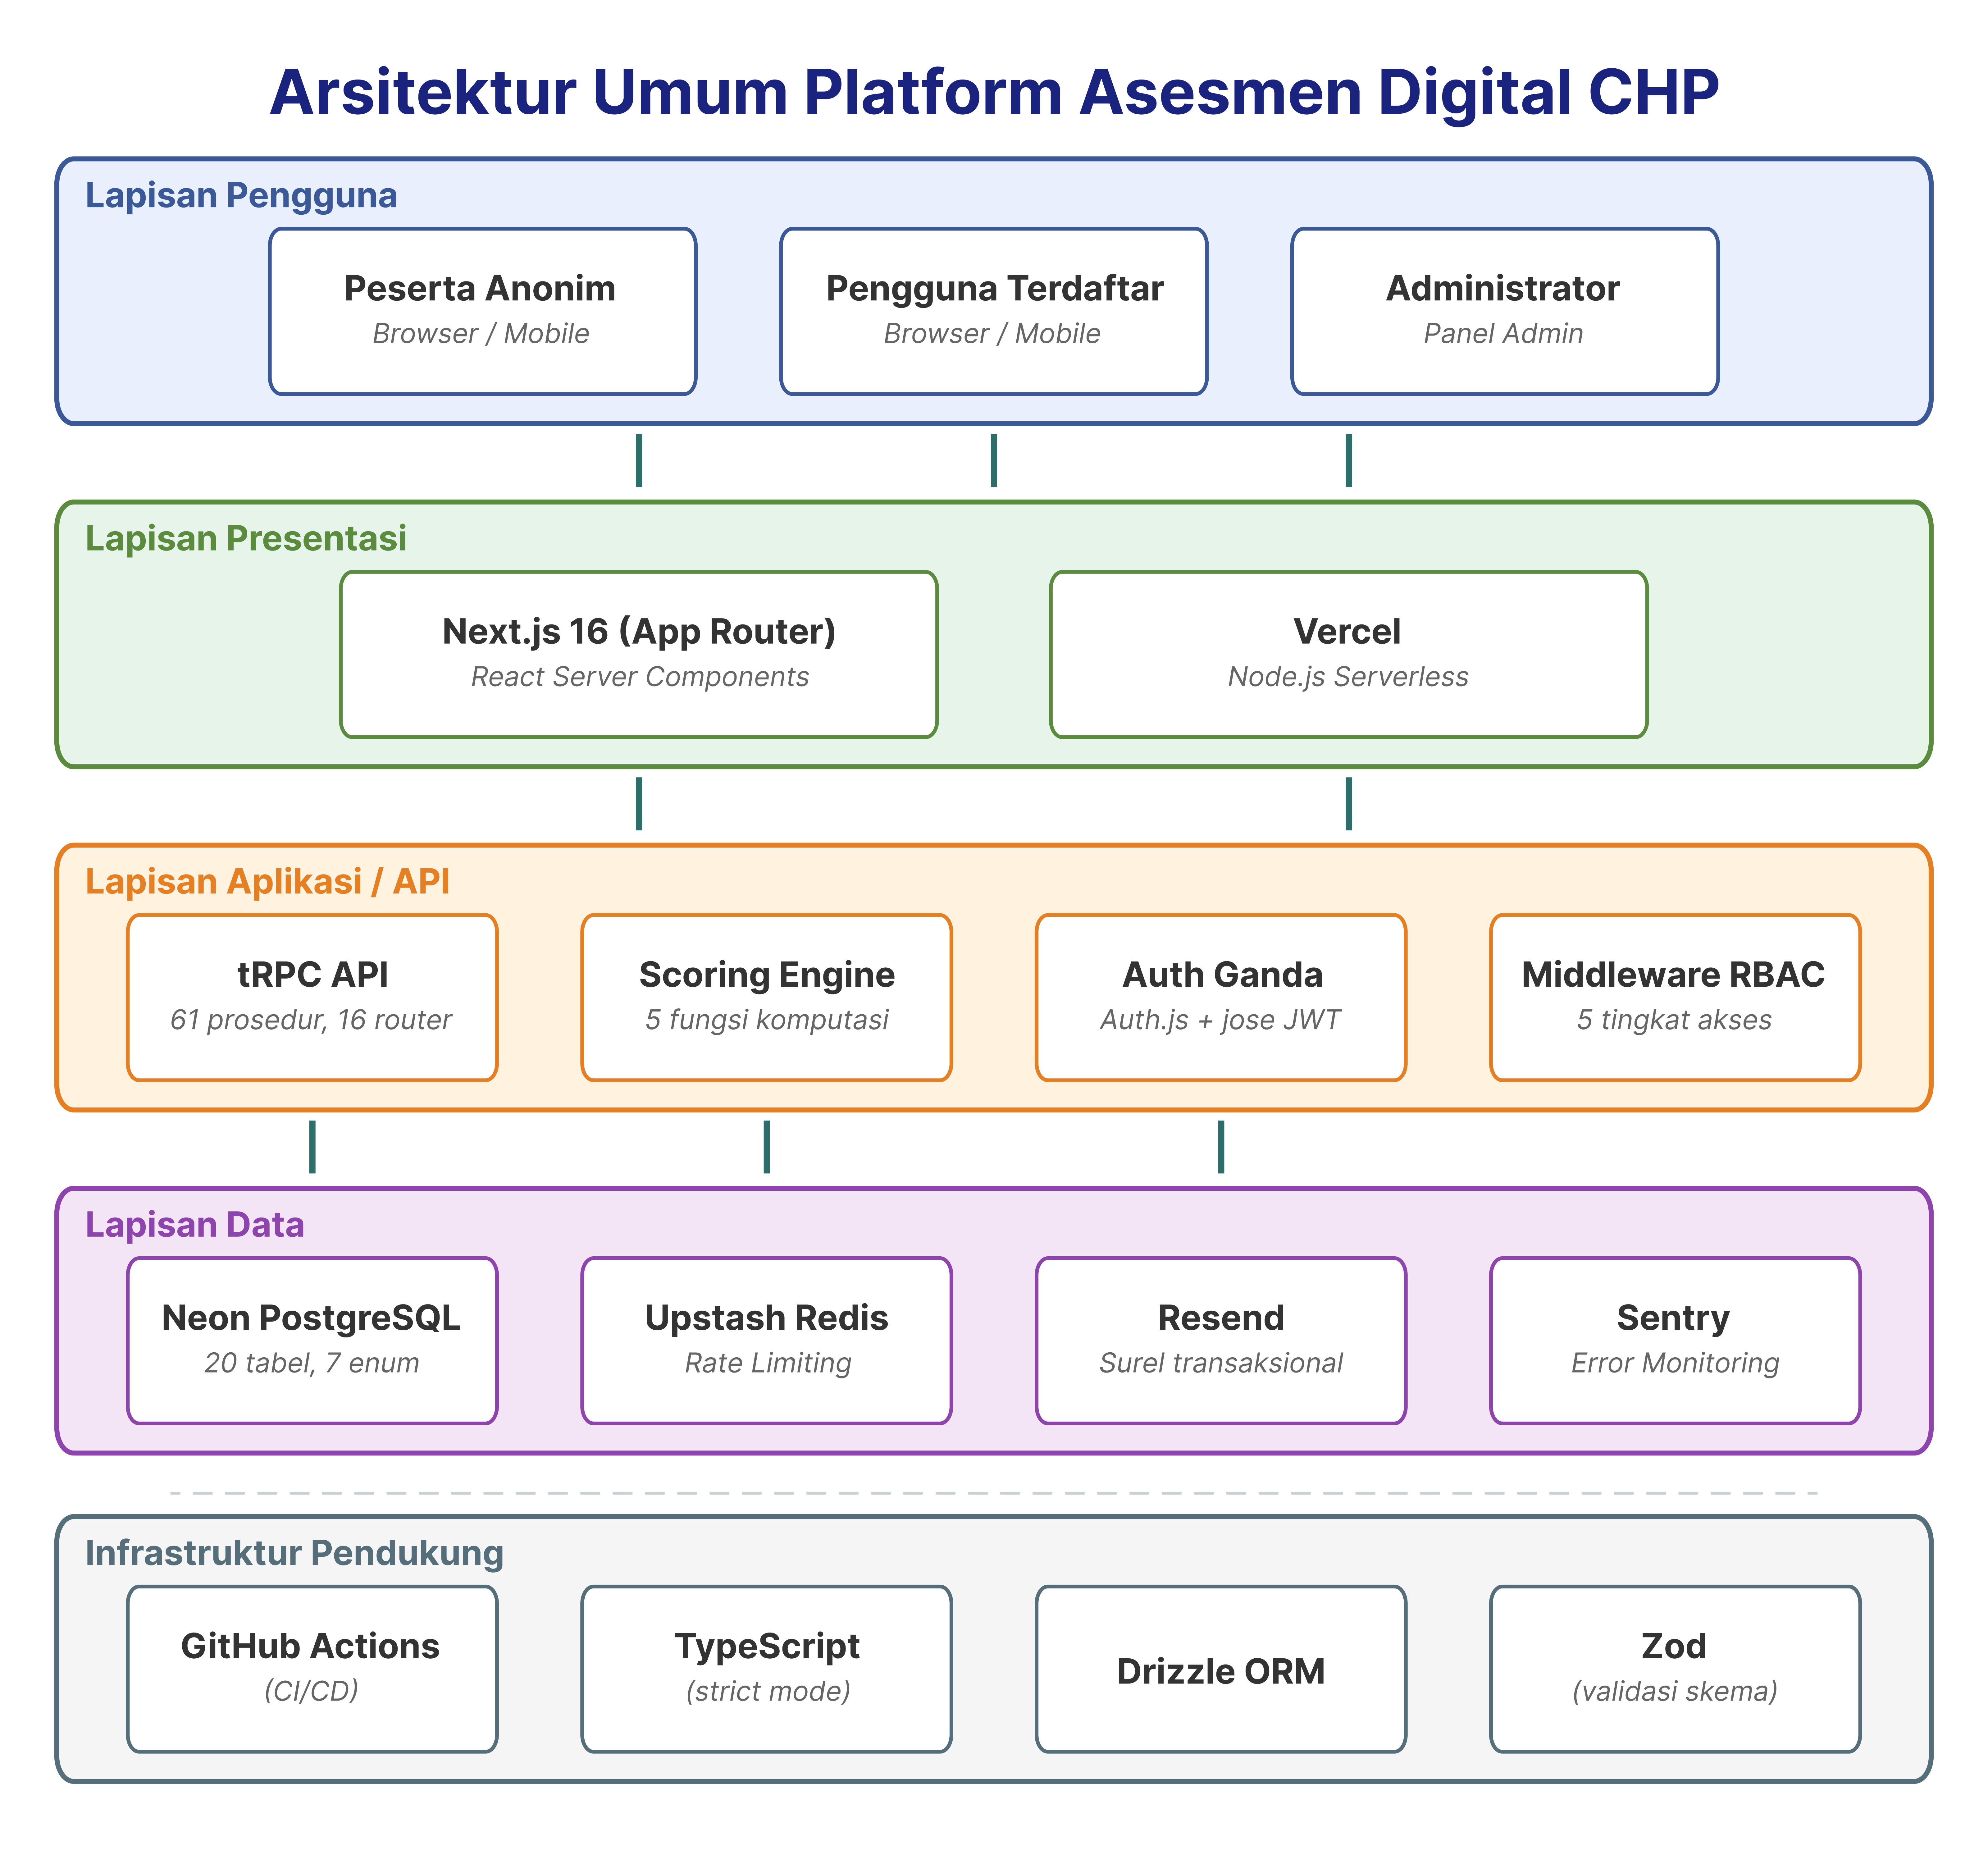
\includegraphics[width=\textwidth]{figures/gambar_1_1_arsitektur_umum.png}
  \caption{Gambaran Umum Arsitektur Platform Asesmen Digital CHP}
  \label{fig:arsitektur-umum}
\end{figure}

% ─────────────────────────────────────────────────────────────────────────────
\section{Skema Kerja Praktik}
\label{sec:skema-kp}

Kerja Praktik (KP) adalah mata kuliah wajib pada Program Studi Informatika UKRIDA yang menekankan aspek kemandirian mahasiswa dalam beradaptasi dengan dunia kerja nyata. Pelaksanaan KP dimaksudkan agar mahasiswa memperoleh pengalaman praktis dalam mengaplikasikan keahliannya di bidang teknologi informasi sekaligus memahami bagaimana suatu instansi dikelola.

KP ini dilaksanakan menggunakan skema Proyek Dosen, yaitu skema di mana mahasiswa terlibat langsung dalam pengembangan produk inovatif milik dosen selaku pemilik proyek. Dosen sebagaimana dimaksud adalah Ibu Astin selaku Ketua Program Studi Psikologi yang sekaligus menjabat sebagai Kepala Riset CHP UKRIDA. Skema Proyek Dosen dipilih karena pengembangan Platform Asesmen Digital CHP merupakan inisiatif riset resmi CHP yang membutuhkan produk \textit{Information Technology} (IT) berupa platform asesmen psikometri digital berkualitas produksi (\textit{production-ready}).

Dalam kerangka proyek ini, penulis bertanggung jawab atas tiga ranah pengembangan utama, yaitu:

\begin{enumerate}[leftmargin=2cm]
  \item Arsitektur sistem: perancangan skema basis data, infrastruktur \textit{Continuous Integration/Continuous Deployment} (CI/CD), dan konfigurasi layanan \textit{cloud}.
  \item \textit{Backend} dan API: implementasi prosedur tRPC, \textit{scoring engine}, dan sistem autentikasi.
  \item Pengujian dan implementasi (\textit{testing and implementation}).
\end{enumerate}

Pengembangan komponen antarmuka pengguna (\textit{User Interface}/UI) dan desain pengalaman pengguna (\textit{User Experience}/UX) dikerjakan secara terpisah oleh anggota tim lain dalam laporan KP tersendiri, sehingga kedua laporan saling melengkapi untuk menggambarkan sistem secara menyeluruh.

% ─────────────────────────────────────────────────────────────────────────────
\section{Tujuan dan Manfaat}
\label{sec:tujuan-manfaat}

Pelaksanaan KP ini memiliki enam tujuan yang dirumuskan menggunakan pendekatan SMART (\textit{Specific, Measurable, Achievable, Relevant, Time-bound}), yaitu spesifik, terukur, dapat dicapai, relevan, dan berbatas waktu. Tabel~\ref{tab:tujuan-kp} menyajikan rumusan tujuan beserta target terukur dan status implementasi pada saat laporan ini disusun.

% [F2] Goals #2, #4, #5, #6 status updated
\begin{longtable}{@{}c p{4cm} p{4.5cm} p{4cm}@{}}
  \caption{Tujuan Kerja Praktik dan Status Implementasi}
  \label{tab:tujuan-kp} \\
  \toprule
  \textbf{No.} & \textbf{Tujuan} & \textbf{Target Terukur} & \textbf{Status} \\
  \midrule
  \endfirsthead
  \toprule
  \textbf{No.} & \textbf{Tujuan} & \textbf{Target Terukur} & \textbf{Status} \\
  \midrule
  \endhead
  \bottomrule
  \endfoot
  1 & Membangun platform asesmen modern dan responsif sesuai standar aksesibilitas & Skor \textit{Lighthouse Performance} $\geq$ 90; \textit{Accessibility} $\geq$ 95 pada semua halaman utama & Selesai: Fase 1A \& 1B (Minggu 1--6) \\[0.5em]
  2 & Mengimplementasikan \textit{scoring engine} modular otomatis untuk perhitungan sumatif, berbobot, dimensional, dan persentil & Skor komputasi sesuai nilai referensi manual; \textit{engine} diuji dengan 72 kasus uji & Selesai: Fase 1B (Minggu 3--6) \\[0.5em]
  3 & Menyajikan umpan balik visual instan berupa skor total, \textit{breakdown} dimensi, dan grafik & Halaman hasil ter-\textit{render} dalam dua detik setelah pengiriman tes & Selesai: Fase 1B (Minggu 5--6) \\[0.5em]
  4 & Membangun fungsionalitas ekspor data berkualitas riset dalam format CSV & Prosedur \texttt{adminResults.export} dengan batas 5000 baris, mencakup jawaban per butir soal & Selesai: Fase 1C (Minggu 7--10) \\[0.5em]
  5 & Mengembangkan panel administrator dengan RBAC & Tim psikologi dapat membuat, mengkonfigurasi, dan mempublikasikan instrumen baru tanpa intervensi pengembang; empat peran admin & Selesai: Fase 1C (Minggu 7--10) \\[0.5em]
  6 & Memastikan serah terima sistem yang berkelanjutan dengan dokumentasi komprehensif & Pengembang baru dapat \textit{clone}, \textit{setup}, dan menjalankan proyek secara lokal dalam waktu 15 menit & Selesai: Fase 1D (Minggu 11--13) \\
\end{longtable}

Adapun manfaat yang diharapkan dari pengembangan Platform Asesmen Digital CHP mencakup empat dimensi utama:

\begin{enumerate}[leftmargin=2cm]
  \item Validitas riset yang meningkat berkat penyimpanan respons mentah yang tidak dapat diubah (\textit{immutable raw responses}) disertai metadata versi instrumen dan versi algoritma penilaian untuk reprodusibilitas ilmiah.
  \item Pengalaman pengguna yang profesional dan aksesibel dengan antarmuka yang menenangkan (\textit{calm design}) sehingga meminimalkan kecemasan peserta tes.
  \item Skalabilitas sistem: untuk menambahkan instrumen psikologi baru secara mandiri melalui panel admin tanpa memerlukan intervensi pengembang.
  \item Keberlanjutan operasional lintas semester: berkat arsitektur yang terdokumentasi secara komprehensif dan kode yang aman secara tipe.
\end{enumerate}

% ─────────────────────────────────────────────────────────────────────────────
\section{Batasan Kerja Praktik}
\label{sec:batasan-kp}

Agar pengerjaan proyek tetap terfokus dan dapat diselesaikan dalam batas waktu yang ditentukan, ruang lingkup pekerjaan ditetapkan sebagai berikut.

Pekerjaan yang termasuk dalam ruang lingkup KP penulis adalah:

\begin{enumerate}[leftmargin=2cm]
  \item Perancangan dan implementasi skema basis data relasional menggunakan Drizzle ORM yang mendukung instrumen psikometri multidimensional, manajemen sesi anonim, dan jejak audit administratif.
  \item Pengembangan infrastruktur CI/CD otomatis menggunakan GitHub Actions dengan dua \textit{job} paralel: \textit{job} pertama menjalankan \textit{linting} (ESLint), \textit{type checking} (TypeScript \textit{Compiler}), dan \textit{build} produksi; \textit{job} kedua menjalankan \textit{unit testing} (Vitest).
  \item Implementasi \textit{scoring engine} modular yang mendukung algoritma penilaian sumatif, berbobot, terbalik (\textit{reversed}), dimensional, dan persentil, sepenuhnya dikonfigurasi melalui basis data.
  \item Pengembangan prosedur API berbasis tRPC untuk manajemen sesi asesmen, penyimpanan jawaban, komputasi skor, autentikasi administrator, dan manajemen instrumen.
  \item Implementasi sistem autentikasi ganda: Auth.js v5 untuk pengguna publik dan JWT mandiri melalui jose untuk panel administrator, dengan \textit{Role-Based Access Control} (RBAC) berlima tingkat.
  \item Pengujian komprehensif mencakup \textit{unit test} pada \textit{scoring engine} dan prosedur API, \textit{integration test} prosedur API, serta pengujian keamanan dasar menggunakan \textit{checklist} OWASP \textit{Top Ten}.
\end{enumerate}

Pekerjaan yang tidak termasuk dalam ruang lingkup KP ini adalah:

\begin{enumerate}[leftmargin=2cm]
  \item Pengembangan aplikasi \textit{mobile native} (iOS/Android): platform bersifat berbasis web (\textit{web-based}) dan responsif untuk perangkat seluler.
  \item Interpretasi hasil berbasis kecerdasan buatan (AI) atau \textit{Large Language Model} (LLM).
  \item Fungsionalitas diagnosis klinis: platform hanya menyediakan \textit{self-assessment} mandiri, bukan diagnosis klinis.
  \item Pengembangan komponen UI dan desain UX, yang merupakan tanggung jawab anggota tim lain dalam laporan KP terpisah.
  \item Fitur aksesibilitas khusus seperti dukungan \textit{screen reader} atau teknologi asistif untuk penyandang disabilitas: fitur ini berada di luar cakupan versi ini dan dicatat sebagai batasan sistem yang dapat dikembangkan pada iterasi berikutnya.
  \item Verifikasi usia responden: sistem tidak membatasi usia pengguna dan tidak dapat memverifikasi apakah responden di bawah umur didampingi oleh orang dewasa. Ini merupakan batasan yang disadari (\textit{known limitation}) dan pengguna diasumsikan mampu membaca instruksi secara mandiri serta mengoperasikan perangkat masukan.
\end{enumerate}

% ─────────────────────────────────────────────────────────────────────────────
\section{Waktu Pelaksanaan}
\label{sec:waktu-pelaksanaan}

Pelaksanaan KP ini berlangsung selama kurang lebih 12 hingga 14 minggu, dimulai pada 11 Februari 2026 melalui koordinasi perdana dengan dosen pemilik proyek hingga direncanakan selesai pada awal Juni 2026 dengan sidang KP. Tabel~\ref{tab:jadwal-kp} menyajikan rincian jadwal pelaksanaan per fase beserta kegiatan utama masing-masing.

% [C1] Changed "16 tabel" → "20 tabel"
\begin{longtable}{@{}p{3.5cm} p{3cm} p{8cm}@{}}
  \caption{Jadwal Pelaksanaan Kerja Praktik}
  \label{tab:jadwal-kp} \\
  \toprule
  \textbf{Fase} & \textbf{Periode} & \textbf{Kegiatan Utama} \\
  \midrule
  \endfirsthead
  \toprule
  \textbf{Fase} & \textbf{Periode} & \textbf{Kegiatan Utama} \\
  \midrule
  \endhead
  \bottomrule
  \endfoot
  Fase 0: Perencanaan & 11 Feb 2026 & Koordinasi perdana, penyusunan rencana proyek (731 baris \textit{unified project plan}), analisis sistem lama \\[0.3em]
  Fase 1A: Fondasi \& \textit{Setup} & Minggu 1--2 & Inisialisasi proyek Next.js, desain skema basis data (20 tabel), konfigurasi CI/CD, \textit{seeding} data awal \\[0.3em]
  Fase 1B: Inti Asesmen & Minggu 3--6 & Katalog tes, mesin asesmen multi-langkah, \textit{scoring engine}, prosedur tRPC, \textit{pre-test} dan \textit{post-test flow} \\[0.3em]
  Fase 2A--2C: Autentikasi & Minggu 4--7 & Infrastruktur JWT ganda, UI autentikasi (\textit{sign-up}, \textit{login}), mutasi \textit{claim session}, migrasi skema Auth.js \\[0.3em]
  Fase 1C: Admin \& \textit{Polish} & Minggu 7--10 & Panel admin dengan RBAC empat peran, CRUD instrumen tes, konfigurasi penilaian, ekspor data \\[0.3em]
  Fase 1D: Pengujian \& Serah Terima & Minggu 11--13 & Pengujian unit (235 kasus uji), pengujian keamanan (OWASP \textit{checklist}), dokumentasi teknis, \textit{deployment} final \\[0.3em]
  Sidang KP & Juni 2026 & Presentasi dan evaluasi akhir di hadapan tim penguji Program Studi Informatika UKRIDA \\
\end{longtable}


% ── BAB II: Landasan Teori ──────────────────────────────────────────────────
% =============================================================================
% 20-bab2.tex — BAB II LANDASAN TEORI
% Patches: C2 (4 roles), C4 (bcryptjs), C5 (5 scoring functions),
%          C6 (2-job CI), C9 (5 auth tiers), C10 (proxy.ts)
% =============================================================================
\chapter{LANDASAN TEORI}
\label{chap:landasan-teori}

Bab ini memaparkan landasan teori yang menjadi dasar ilmiah dan teknis dalam perancangan serta implementasi Platform Asesmen Digital CHP. Sesuai dengan fokus penulis pada arsitektur sistem, pengembangan \textit{backend}, dan pengujian perangkat lunak, teori yang dibahas mencakup rekayasa perangkat lunak dengan metodologi Agile, arsitektur sistem web modern berbasis Next.js, pengembangan \textit{backend} dengan tRPC dan PostgreSQL, sistem autentikasi dan otorisasi, strategi pengujian perangkat lunak, serta keamanan dan privasi data.

% ─────────────────────────────────────────────────────────────────────────────
\section{Rekayasa Perangkat Lunak}
\label{sec:rekayasa-pl}

Rekayasa Perangkat Lunak (\textit{Software Engineering}) adalah disiplin ilmu teknik yang berkaitan dengan semua aspek produksi perangkat lunak, mulai dari tahap spesifikasi awal sistem hingga pemeliharaan sistem setelah digunakan (Sommerville 2016). Rekayasa perangkat lunak mencakup manajemen proyek, proses pengembangan, metode teknis, dan penggunaan alat (\textit{tools}) yang tepat guna menghasilkan perangkat lunak yang dapat diandalkan, efisien, dan memenuhi kebutuhan penggunanya.

Proses rekayasa perangkat lunak pada umumnya melibatkan empat aktivitas fundamental yang saling berkaitan, yaitu: (1) spesifikasi perangkat lunak, yaitu pendefinisian fungsionalitas dan kendala operasi sistem; (2) pengembangan perangkat lunak, yaitu perancangan dan pemrograman sistem sesuai spesifikasi; (3) validasi perangkat lunak, yaitu pemastian bahwa sistem memenuhi kebutuhan pengguna; serta (4) evolusi perangkat lunak, yaitu modifikasi sistem sebagai respons terhadap perubahan kebutuhan. Pada proyek Platform CHP, keempat aktivitas ini dilaksanakan secara iteratif dalam kerangka metodologi Agile.

\subsection{Model Proses: Metodologi Agile}
\label{subsec:agile}

Model proses perangkat lunak mendefinisikan pendekatan yang digunakan untuk mengorganisasi dan mengelola aktivitas pengembangan. Dalam proyek ini, model Agile iteratif dan inkremental dipilih sebagai kerangka kerja pengembangan. Agile adalah sekumpulan nilai dan prinsip yang diformulasikan dalam \textit{Agile Manifesto} (2001), yang menekankan respons terhadap perubahan di atas mengikuti rencana yang kaku, kolaborasi erat dengan pelanggan di atas negosiasi kontrak, dan penyerahan perangkat lunak yang berfungsi di atas dokumentasi yang ekstensif.

Manifestasi Agile yang digunakan dalam proyek ini adalah Scrum, sebuah kerangka kerja manajemen proyek yang mengorganisasi pekerjaan ke dalam siklus waktu tetap yang disebut \textit{sprint} (Schwaber dan Sutherland 2020). Setiap \textit{sprint} pada proyek CHP berdurasi dua minggu. Pada setiap akhir \textit{sprint}, tim menghasilkan \textit{increment} (versi perangkat lunak yang siap didemonstrasikan dan berpotensi untuk dirilis). Dalam konteks KP ini, pertemuan dua mingguan dengan Ibu Astin selaku pemilik proyek berfungsi sebagai sesi \textit{sprint review}, di mana demonstrasi fitur yang telah diimplementasikan disampaikan untuk mendapatkan umpan balik langsung.

Pemilihan Agile untuk proyek ini didasari tiga pertimbangan utama:

\begin{enumerate}[leftmargin=2cm]
  \item Jadwal tetap 12 minggu menuntut penyerahan fitur secara inkremental, sehingga pemangku kepentingan dapat menggunakan dan memberikan umpan balik terhadap fitur yang sudah selesai sembari fitur lain masih dikembangkan.
  \item Kebutuhan instrumen psikometri dari tim psikologi dapat berevolusi selama pengembangan, dan Agile mengakomodasi perubahan ini tanpa memerlukan renegosiasi kontrak formal.
  \item Tim kecil yang terdiri atas dua pengembang cocok dengan prinsip Agile yang mengutamakan komunikasi langsung dan minimalisasi birokrasi proses.
\end{enumerate}

% ─────────────────────────────────────────────────────────────────────────────
\section{Arsitektur Sistem Web Modern}
\label{sec:arsitektur-web}

Arsitektur sistem web mengacu pada struktur tingkat tinggi dari sebuah aplikasi web yang mendefinisikan bagaimana komponen-komponen penyusunnya diorganisasi, berinteraksi, dan berkomunikasi satu sama lain.

\subsection{Arsitektur Tiga Lapisan}
\label{subsec:three-tier}

Arsitektur tiga lapisan (\textit{three-tier architecture}) adalah pola arsitektur yang membagi aplikasi menjadi tiga lapisan logis yang terpisah: lapisan presentasi (\textit{presentation tier}), lapisan aplikasi (\textit{application tier}), dan lapisan data (\textit{data tier}). Pemisahan ini menerapkan prinsip \textit{separation of concerns} yang memungkinkan setiap lapisan untuk dikembangkan, diuji, dan diskalakan secara independen.

Pada Platform Asesmen Digital CHP, ketiga lapisan diimplementasikan sebagai berikut:

\begin{enumerate}[leftmargin=2cm]
  \item Lapisan Presentasi: Komponen React dengan \textit{React Server Components} (RSC), Tailwind CSS, dan shadcn/ui yang menghasilkan antarmuka pengguna interaktif dan responsif.
  \item Lapisan Aplikasi: \textit{Router} tRPC, \textit{scoring engine}, \textit{middleware} autentikasi, dan \textit{Server Actions} yang mengandung seluruh logika bisnis sistem.
  \item Lapisan Data: PostgreSQL yang diakses melalui Drizzle ORM sebagai sumber data utama, dengan Upstash Redis sebagai lapisan \textit{caching} dan \textit{rate limiting}.
\end{enumerate}

Gambar~\ref{fig:arsitektur-3-tier} mengilustrasikan diagram arsitektur tiga lapisan Platform CHP.

\begin{figure}[htbp]
  \centering
  \includegraphics[width=\textwidth]{figures/gambar_2_1_arsitektur_tiga_lapisan.png}
  \caption{Diagram Arsitektur Tiga Lapisan Platform Asesmen Digital CHP}
  \label{fig:arsitektur-3-tier}
\end{figure}

\subsection{Next.js dan \textit{React Server Components}}
\label{subsec:nextjs}

Next.js adalah \textit{meta-framework} berbasis React yang menyediakan fondasi lengkap untuk membangun aplikasi web \textit{full-stack} modern (Vercel 2026). Proyek ini menggunakan Next.js 16 dengan \textit{App Router} yang membawa pergeseran arsitektural signifikan melalui \textit{React Server Components} (RSC).

RSC adalah paradigma \textit{rendering} yang memungkinkan komponen React dieksekusi dan di-\textit{render} secara eksklusif di sisi server, tanpa mengirimkan kode JavaScript komponen tersebut ke \textit{browser} klien. Implikasi praktis RSC untuk Platform CHP adalah pengurangan ukuran \textit{bundle} JavaScript yang dikirim ke \textit{browser} peserta tes. Komponen yang hanya membaca data, seperti halaman katalog tes, halaman informasi, dan halaman hasil, di-\textit{render} di server tanpa mengirimkan kodenya ke klien. Hanya komponen yang memerlukan interaktivitas, seperti formulir asesmen dan tombol navigasi, yang ditandai dengan direktif \texttt{"use client"} dan dikirim ke \textit{browser}.

% ─────────────────────────────────────────────────────────────────────────────
\section{TypeScript dan Keamanan Tipe}
\label{sec:typescript}

TypeScript adalah bahasa pemrograman \textit{open-source} yang dikembangkan oleh Microsoft sebagai \textit{superset} dari JavaScript. TypeScript menambahkan sistem pengetikan statis (\textit{static type system}) di atas JavaScript, sehingga setiap variabel, parameter fungsi, dan nilai kembalian dapat diberikan anotasi tipe eksplisit.

\subsection{Signifikansi TypeScript dalam Proyek CHP}
\label{subsec:typescript-chp}

Sebuah studi berskala besar terhadap 85 proyek web oleh Bogner dan Merkel (2022) menunjukkan bahwa penggunaan TypeScript menurunkan densitas \textit{code smell} sebesar 34\% dan mengurangi kompleksitas kognitif sebesar 28\% dibandingkan JavaScript murni (Bogner dan Merkel 2022). Studi lain (arXiv 2026) mengungkap bahwa pengetikan statis mengubah lanskap kegagalan pada aplikasi modern: mayoritas \textit{bug} dalam proyek ekosistem TypeScript bersumber dari kesalahan konfigurasi \textit{toolchains}, penyalahgunaan integrasi antarmuka API, dan kegagalan penanganan status asinkron.

Pada Platform CHP, TypeScript digunakan di seluruh \textit{codebase} dengan konfigurasi \texttt{strict: true} yang mengaktifkan pemeriksaan tipe paling ketat. Setiap prosedur tRPC mendefinisikan skema masukan dan keluaran menggunakan pustaka validasi Zod, yang secara otomatis menghasilkan tipe TypeScript.

% ─────────────────────────────────────────────────────────────────────────────
\section{Backend dan Basis Data}
\label{sec:backend-db}

\subsection{PostgreSQL dan Basis Data \textit{Serverless}}
\label{subsec:postgresql}

PostgreSQL adalah sistem manajemen basis data relasional \textit{open-source} yang dikenal karena kepatuhannya terhadap standar SQL, ekstensibilitas, dan dukungan terhadap tipe data kompleks seperti JSONB (PostgreSQL Global Development Group 2026). Platform CHP menggunakan PostgreSQL 17 melalui layanan \textit{serverless} Neon yang memisahkan komputasi dari penyimpanan, memungkinkan basis data untuk diskalakan ke nol saat tidak ada permintaan dan aktif kembali dalam hitungan milidetik.

\subsection{Drizzle ORM dan Perancangan Skema}
\label{subsec:drizzle}

Drizzle ORM adalah ORM TypeScript generasi baru yang berfilosofi ``SQL-\textit{first}'', sintaksis API-nya dirancang semirip mungkin dengan SQL namun sepenuhnya aman secara tipe (Drizzle Team 2026). Skema basis data Platform CHP dirancang untuk mendukung instrumen psikometri yang fleksibel. Tabel~\ref{tab:ringkasan-skema} menyajikan ringkasan tabel-tabel utama.

\begin{table}[htbp]
  \centering
  \caption{Ringkasan Skema Basis Data Platform CHP}
  \label{tab:ringkasan-skema}
  \begin{tabularx}{\textwidth}{@{}p{3cm} p{4.5cm} X@{}}
    \toprule
    \textbf{Nama Tabel} & \textbf{Kolom Kunci} & \textbf{Tujuan} \\
    \midrule
    \texttt{tests} & id, slug, title, version & Metadata instrumen psikometri dengan kontrol versi \\
    \texttt{questions} & id, test\_id, type, dimension, is\_reversed, weight & Butir soal dengan informasi dimensi dan pembobotan \\
    \texttt{scoring\_rules} & id, test\_id, algorithm, config & Konfigurasi algoritma penilaian \\
    \texttt{test\_sessions} & id, test\_id, status, ip\_hash, claim\_token & Sesi asesmen dengan mekanisme klaim \\
    \texttt{answers} & id, session\_id, question\_id, value & Respons mentah yang \textit{immutable} \\
    \texttt{results} & id, session\_id, total\_score, dimension\_scores & Skor terhitung yang terpisah dari respons mentah \\
    \texttt{audit\_logs} & id, admin\_user\_id, action, entity\_type & Jejak audit untuk akuntabilitas \\
    \bottomrule
  \end{tabularx}
\end{table}

Keputusan arsitektur terpenting adalah pemisahan tabel \texttt{answers} dari tabel \texttt{results}. Dengan menyimpan respons mentah secara permanen dan terpisah dari skor yang telah dihitung, tim psikologi dapat melakukan \textit{re-scoring} menggunakan algoritma yang diperbarui tanpa kehilangan data historis asli.

\subsection{tRPC}
\label{subsec:trpc}

tRPC (\textit{TypeScript Remote Procedure Call}) adalah \textit{framework} yang memungkinkan pembuatan API yang sepenuhnya aman secara tipe tanpa memerlukan generasi kode atau skema terpisah (tRPC Team 2026). Pada Platform CHP, prosedur tRPC diorganisasi ke dalam \textit{router} berdasarkan domain bisnis:

\begin{enumerate}[leftmargin=2cm]
  \item Router sesi asesmen: Prosedur \texttt{startSession}, \texttt{saveProgress}, dan \texttt{submitAssessment} yang mengelola siklus hidup sesi tes.
  \item Router autentikasi: Prosedur yang menangani registrasi, login, dan klaim sesi anonim ke akun terdaftar.
  \item Router admin: Prosedur yang dilindungi oleh \textit{middleware} RBAC untuk operasi CRUD instrumen tes, konfigurasi penilaian, dan ekspor data.
\end{enumerate}

% ─────────────────────────────────────────────────────────────────────────────
\section{Autentikasi dan Otorisasi}
\label{sec:auth}

Autentikasi (\textit{authentication}) adalah proses verifikasi identitas pengguna, sedangkan otorisasi (\textit{authorization}) menentukan apa yang diizinkan dilakukan oleh pengguna yang telah terautentikasi. Gambar~\ref{fig:auth-flow} mengilustrasikan alur autentikasi dan otorisasi pada Platform CHP.

\begin{figure}[htbp]
  \centering
  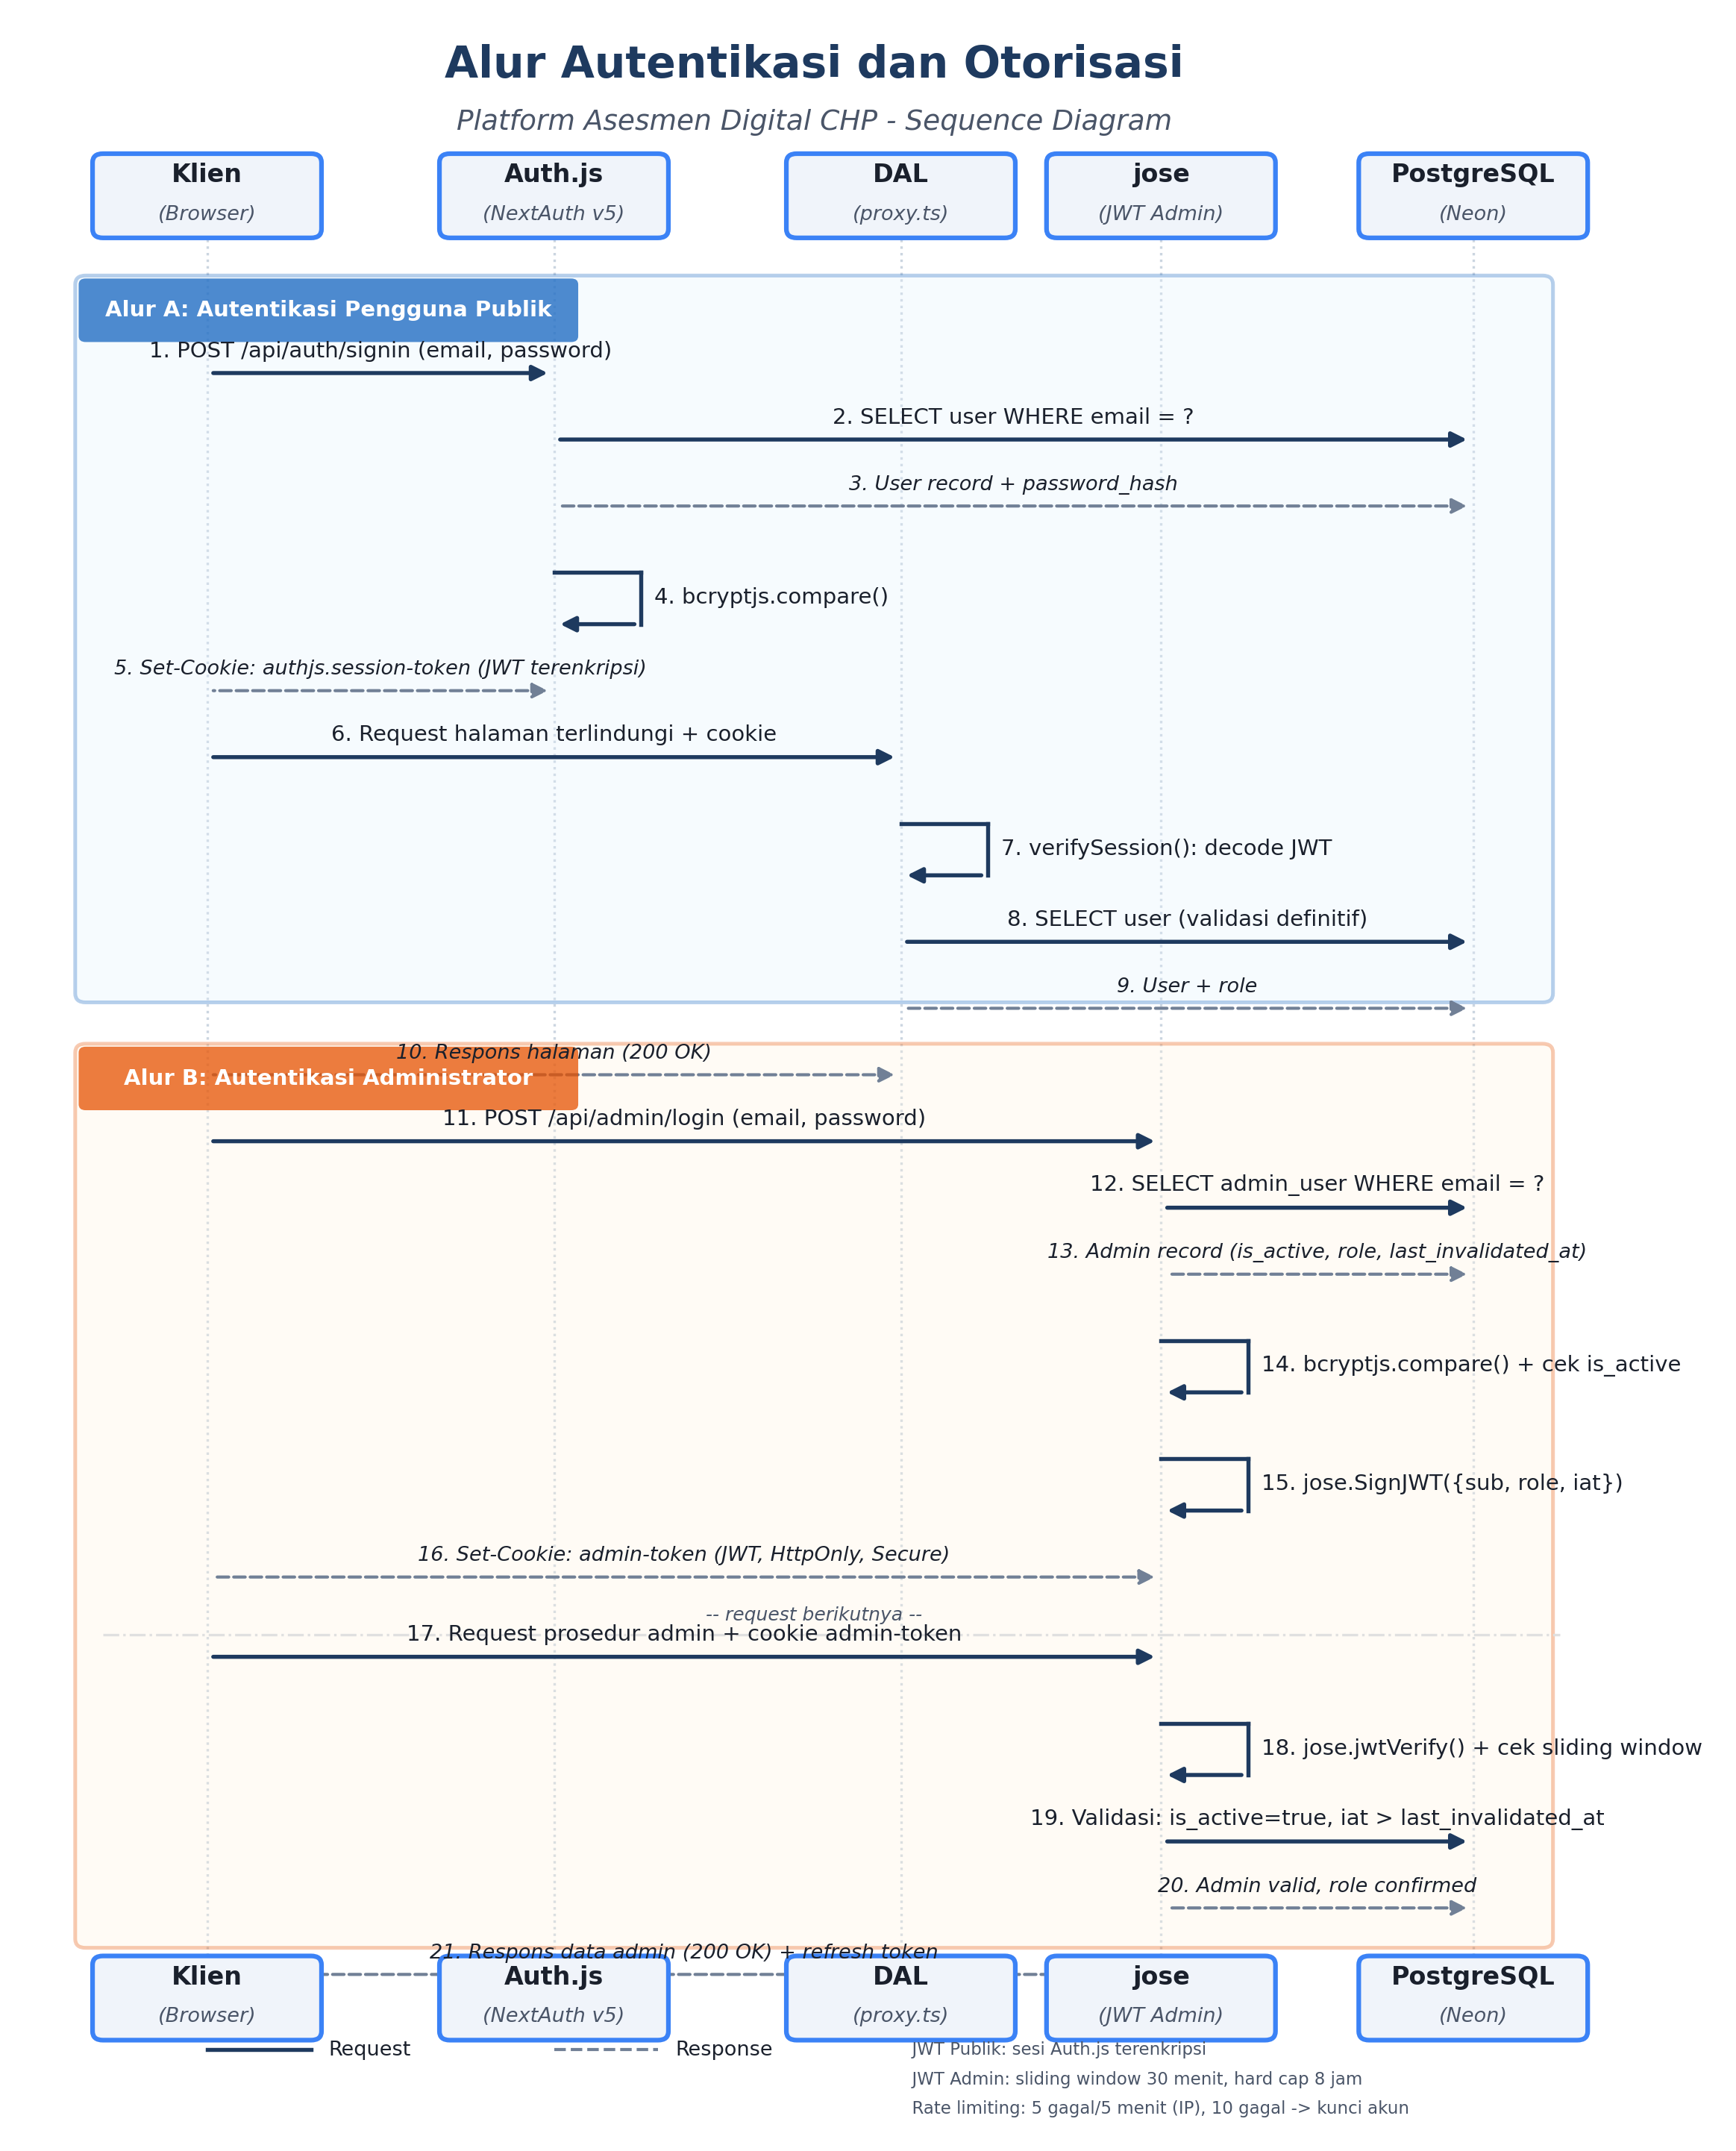
\includegraphics[width=\textwidth]{figures/gambar_2_2_alur_autentikasi.png}
  \caption{Alur Autentikasi dan Otorisasi Platform CHP (\textit{Sequence Diagram})}
  \label{fig:auth-flow}
\end{figure}

\subsection{JSON \textit{Web Token} (JWT)}
\label{subsec:jwt}

\textit{JSON Web Token} (JWT) adalah standar terbuka yang didefinisikan dalam RFC 7519 untuk mentransmisikan informasi secara aman antara pihak-pihak sebagai objek JSON yang ringkas dan mandiri (Jones, Bradley, dan Sakimura 2015). Sebuah JWT terdiri atas tiga bagian: Header (metadata \textit{token}), Payload (klaim tentang pengguna), dan Signature (tanda tangan digital).

Platform CHP mengimplementasikan sistem autentikasi ganda berbasis JWT:

\begin{enumerate}[leftmargin=2cm]
  \item \textbf{Autentikasi pengguna publik} melalui Auth.js (NextAuth v5) dengan \textit{CredentialsProvider}, di mana sesi pengguna disimpan dalam JWT terenkripsi dengan strategi sesi JWT.
  \item \textbf{Autentikasi administrator} melalui pustaka jose secara mandiri (terpisah dari Auth.js), dengan \textit{sliding window} 30 menit dan batas keras (\textit{hard cap}) 8 jam dari waktu penerbitan awal. JWT administrator disimpan dalam \textit{cookie} bernama \texttt{admin-token}.
\end{enumerate}

% [C2] Fixed: "dua peran" → empat peran with correct names
\subsection{\textit{Role-Based Access Control} (RBAC)}
\label{subsec:rbac}

\textit{Role-Based Access Control} (RBAC) adalah model kontrol akses di mana izin diberikan kepada peran tertentu, dan pengguna mendapatkan izin melalui keanggotaan dalam peran yang relevan. RBAC menerapkan prinsip hak istimewa minimal (\textit{principle of least privilege}).

Platform CHP mendefinisikan empat peran untuk pengguna panel admin melalui \textit{enum} PostgreSQL \texttt{admin\_role}:

\begin{enumerate}[leftmargin=2cm]
  \item \textbf{Super Admin} (\texttt{super\_admin}): Memiliki akses penuh terhadap semua operasi, termasuk manajemen akun admin, konfigurasi sistem, dan kemampuan menghapus data.
  \item \textbf{Admin} (\texttt{admin}): Memiliki akses untuk mengelola instrumen tes, melihat data respons sesi, dan mengekspor data penelitian, namun tidak dapat mengelola pengguna admin lain.
  \item \textbf{Psikiater} (\texttt{psychiatrist}): Memiliki akses untuk melihat hasil asesmen dan menyetujui permintaan laporan, dengan fokus pada evaluasi klinis.
  \item \textbf{Peneliti} (\texttt{researcher}): Memiliki akses baca terhadap data riset dan statistik untuk keperluan penelitian, tanpa kemampuan mengubah konfigurasi sistem.
\end{enumerate}

% [C9] Fixed: 3 → 5 middleware levels
Pemeriksaan otorisasi RBAC diimplementasikan pada lapisan \textit{middleware} prosedur tRPC menggunakan lima tingkat kontrol akses:

\begin{enumerate}[leftmargin=2cm]
  \item \texttt{publicProcedure}: tidak memerlukan autentikasi. Digunakan untuk prosedur asesmen dan hasil.
  \item \texttt{protectedProcedure}: memerlukan sesi Auth.js yang valid. Digunakan untuk operasi yang memerlukan identitas pengguna (klaim sesi, profil, riwayat).
  \item \texttt{adminProcedure}: memvalidasi JWT admin melalui jose, memeriksa status aktif dan waktu invalidasi sesi di basis data, serta menerapkan \textit{sliding window refresh}. Digunakan untuk operasi baca pada panel admin.
  \item \texttt{adminMutationProcedure}: memperluas \texttt{adminProcedure} dengan membatasi akses hanya kepada peran \texttt{super\_admin} dan \texttt{admin}. Digunakan untuk operasi tulis pada instrumen tes dan konfigurasi.
  \item \texttt{superAdminProcedure}: memperluas \texttt{adminProcedure} dengan membatasi akses secara eksklusif kepada peran \texttt{super\_admin}. Digunakan untuk manajemen akun admin dan operasi keamanan.
\end{enumerate}

% ─────────────────────────────────────────────────────────────────────────────
\section{Pengujian Perangkat Lunak}
\label{sec:pengujian}

Pengujian perangkat lunak adalah proses evaluasi dan verifikasi bahwa produk perangkat lunak melakukan apa yang seharusnya dilakukan. Pengujian yang komprehensif amat penting untuk Platform CHP mengingat kekritisan akurasi skor dalam konteks penelitian psikometri.

% --- Professor-approved: Testing methodologies (B2.1) ---
\subsection{Metodologi Pengujian}
\label{subsec:metodologi-pengujian}

Dua metodologi pengujian utama digunakan dalam proyek ini. \textit{White-box testing} (pengujian kotak putih, juga dikenal sebagai pengujian struktural) adalah teknik pengujian di mana penguji memiliki akses penuh terhadap kode sumber dan struktur internal sistem (Capote 2023; Bhat dan Khan 2021). Penguji merancang kasus uji berdasarkan pengetahuan tentang jalur eksekusi, kondisi percabangan, dan aliran data dalam kode. \textit{Black-box testing} (pengujian kotak hitam, juga dikenal sebagai pengujian fungsional atau pengujian perilaku) adalah teknik pengujian di mana penguji hanya mengetahui masukan dan keluaran yang diharapkan, tanpa akses terhadap implementasi internal (Capote 2023; Khan dan Khan 2022).

Platform CHP menggunakan pendekatan gabungan: \textit{white-box testing} diterapkan pada \textit{scoring engine} untuk memverifikasi setiap jalur komputasi (pembalikan skor, pengelompokan dimensional, penanganan kasus tepi), sedangkan \textit{black-box testing} diterapkan pada alur pengguna secara keseluruhan (mengisi asesmen, menerima hasil, mengelola instrumen). Tabel~\ref{tab:metodologi-testing} menyajikan pemetaan metodologi pengujian yang digunakan.

\begin{table}[htbp]
  \centering
  \caption{Pemetaan Metodologi Pengujian Platform CHP}
  \label{tab:metodologi-testing}
  \begin{tabularx}{\textwidth}{@{}p{2.5cm} p{2.5cm} X p{2cm}@{}}
    \toprule
    \textbf{Metodologi} & \textbf{Level} & \textbf{Komponen} & \textbf{Alat} \\
    \midrule
    \textit{White-box} & \textit{Unit} & \textit{Scoring engine}, validasi, enkripsi & Vitest \\
    \textit{White-box} & Integrasi & tRPC $\leftrightarrow$ DB, Auth $\leftrightarrow$ RBAC & Vitest \\
    \textit{Black-box} & \textit{End-to-end} & Alur asesmen, alur admin & Playwright \\
    \textit{Black-box} & Validasi & Akurasi skor vs.\ panduan manual & Vitest \\
    \bottomrule
  \end{tabularx}
\end{table}

% --- Professor-approved: Testing pyramid (B2.2) ---
\subsection{Strategi Piramida Pengujian}
\label{subsec:piramida-testing}

Strategi pengujian Platform CHP mengikuti konsep piramida pengujian (\textit{testing pyramid}) yang dipopulerkan oleh Cohn (2009). Piramida pengujian menempatkan \textit{unit test} pada dasar piramida (jumlah terbanyak, eksekusi tercepat, biaya terendah), \textit{integration test} di tengah, dan \textit{end-to-end test} di puncak (jumlah paling sedikit, eksekusi paling lambat, biaya tertinggi). Pendekatan ini memaksimalkan cakupan pengujian sembari meminimalkan waktu eksekusi dan biaya pemeliharaan (Desai, Singh, dan Amilkanthwar 2025). Gambar~\ref{fig:piramida-testing} mengilustrasikan hierarki ini.

\begin{figure}[htbp]
  \centering
  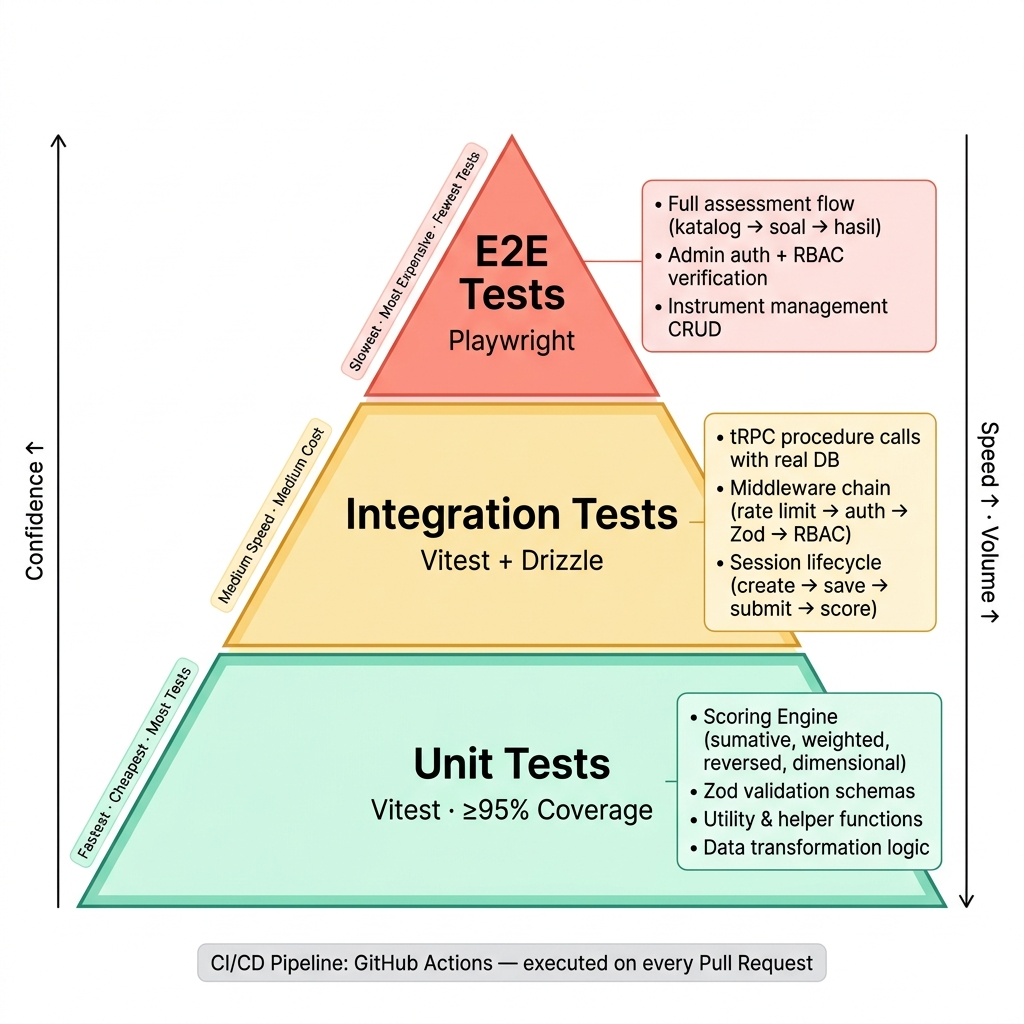
\includegraphics[width=\textwidth]{figures/gambar_2_3_piramida_pengujian.png}
  \caption{Piramida Pengujian Platform Asesmen Digital CHP}
  \label{fig:piramida-testing}
\end{figure}

% --- Professor-approved: Integration testing (B2.3) ---
\subsection{\textit{Integration Testing}}
\label{subsec:integration-testing}

\textit{Integration testing} pada Platform CHP menggunakan metodologi \textit{grey-box}: penguji mengetahui arsitektur internal (skema basis data, kontrak tRPC) namun menguji prosedur sebagai unit fungsional yang utuh. Tiga area fokus integrasi:

\begin{enumerate}[leftmargin=2cm]
  \item \textbf{tRPC $\leftrightarrow$ Basis Data}: memverifikasi bahwa prosedur tRPC menulis dan membaca data yang benar dari PostgreSQL melalui Drizzle ORM, termasuk transaksi atomik dan \textit{constraint} referensial.
  \item \textbf{Autentikasi $\leftrightarrow$ RBAC}: memverifikasi bahwa setiap tingkat \textit{middleware} (dari \texttt{publicProcedure} hingga \texttt{superAdminProcedure}) secara benar mengizinkan atau menolak akses berdasarkan peran pengguna.
  \item \textbf{Validasi Zod $\leftrightarrow$ Logika Bisnis}: memverifikasi bahwa skema masukan Zod menolak data yang tidak valid sebelum logika bisnis dieksekusi, serta bahwa pesan kesalahan yang dikembalikan informatif dan konsisten.
\end{enumerate}

% --- Professor-approved: Validation testing (B2.4) ---
\subsection{Pengujian Validasi: Akurasi Skor Otomatis}
\label{subsec:validation-testing}

Dalam konteks platform asesmen psikometri, pengujian validasi memiliki signifikansi yang melampaui pengujian perangkat lunak konvensional. Skor yang dihasilkan oleh \textit{scoring engine} harus identik dengan skor yang dihitung secara manual menggunakan panduan penilaian (\textit{scoring guide}) resmi masing-masing instrumen (Liu, Chen, dan Sun 2016). Pengujian validasi dilaksanakan dengan membandingkan keluaran \textit{scoring engine} terhadap tabel referensi yang dihitung secara manual untuk setiap instrumen, memverifikasi keidentikan skor (\textit{score identity accuracy}). Selain akurasi, efisiensi waktu juga diukur: komputasi skor otomatis yang sebelumnya memerlukan hitungan menit secara manual kini diselesaikan dalam hitungan milidetik.

\subsection{\textit{Unit Testing} dengan Vitest}
\label{subsec:vitest}

Vitest adalah \textit{framework unit testing} berbasis Vite yang dirancang khusus untuk ekosistem TypeScript/JavaScript modern. Vitest menggunakan model eksekusi yang kompatibel dengan Jest namun dengan kecepatan yang lebih tinggi berkat eksekusi langsung tanpa proses kompilasi TypeScript berulang.

% [C5] Listed all 5 exported functions
Modul \textit{scoring engine} menjadi prioritas utama \textit{unit testing} pada Platform CHP. \textit{Scoring engine} terdiri atas tiga \textit{file} dengan lima fungsi yang diekspor:

\begin{enumerate}[leftmargin=2cm]
  \item \texttt{reverseScore(rawValue, options)}: menghitung skor terbalik secara agnostik skala: $(\text{scaleMax} - \text{rawValue}) + \text{scaleMin}$.
  \item \texttt{computeScore(input)}: fungsi inti yang menangani pembalikan butir soal, penjumlahan berbobot, pengelompokan dimensional, \textit{rollup} orde kedua untuk DSR (GPIUS-2), dan komputasi \texttt{maxPossibleScore}.
  \item \texttt{lookupInterpretation(testId, totalScore, dimension?)} : mengkueri tabel \texttt{result\_interpretations} untuk pemetaan skor ke label, deskripsi, rekomendasi, dan tingkat keparahan.
  \item \texttt{validateAnswerValues(answers, questions)} : memvalidasi bahwa setiap nilai jawaban berada dalam batas opsi yang valid. Fungsi murni tanpa akses basis data.
  \item \texttt{validateCompleteness(answers, questions)} : memvalidasi bahwa semua butir soal wajib telah dijawab. Fungsi murni tanpa akses basis data.
\end{enumerate}

Tabel~\ref{tab:skenario-unit-test} menampilkan contoh skenario \textit{unit test} yang diimplementasikan.

\begin{table}[htbp]
  \centering
  \caption{Contoh Skenario \textit{Unit Test} pada \textit{Scoring Engine}}
  \label{tab:skenario-unit-test}
  \begin{tabularx}{\textwidth}{@{}p{3.5cm} X X@{}}
    \toprule
    \textbf{Fungsi} & \textbf{Kondisi Masukan} & \textbf{Hasil yang Diharapkan} \\
    \midrule
    \texttt{computeScore} (sumatif) & 5 soal dengan nilai 4, 3, 5, 2, 4 & totalScore = 18 \\
    \texttt{computeScore} (terbalik) & Soal is\_reversed=true, skala 1--5, jawaban 2 & Skor soal menjadi 4 $(5+1-2)$ \\
    \texttt{computeScore} (dimensional) & 10 soal: 5 dimensi A, 5 dimensi B & dimensionScores terpisah per dimensi \\
    \texttt{\seqsplit{validateCompleteness}} & Satu soal wajib belum dijawab & valid = false, missingQuestionIds berisi ID soal \\
    \bottomrule
  \end{tabularx}
\end{table}

\subsection{\textit{End-to-End Testing} dengan Playwright}
\label{subsec:playwright}

Playwright adalah \textit{framework} otomasi \textit{browser} yang dikembangkan oleh Microsoft untuk E2E \textit{testing}. Tiga alur kritis yang menjadi prioritas E2E \textit{testing} adalah: (1) alur asesmen penuh dari katalog hingga halaman hasil; (2) alur autentikasi admin termasuk \textit{redirect} otomatis; dan (3) alur manajemen instrumen dari pembuatan hingga publikasi.

% [C6] Fixed: "4 gate sequential" → 2 parallel jobs
\subsection{CI/CD dengan GitHub Actions}
\label{subsec:cicd}

\textit{Continuous Integration/Continuous Deployment} (CI/CD) menghilangkan proses integrasi dan \textit{deployment} manual yang rawan kesalahan. Platform CHP mengimplementasikan \textit{pipeline} CI/CD menggunakan GitHub Actions yang diaktifkan pada setiap \textit{pull request} dan \textit{push} ke cabang utama \texttt{master}.

\textit{Pipeline} terdiri atas dua \textit{job} yang berjalan secara paralel:

\begin{enumerate}[leftmargin=2cm]
  \item \textbf{\textit{Job} 1: \texttt{build-and-test}}: menjalankan tiga \textit{gate} secara berurutan:
  \begin{enumerate}
    \item Pemeriksaan \textit{linting} (ESLint): memastikan konsistensi gaya kode.
    \item Pemeriksaan \textit{type checking} (TypeScript \textit{Compiler} dengan \textit{strict mode}): memastikan tidak ada kesalahan tipe.
    \item Proses \textit{build} produksi (Next.js): memastikan aplikasi dapat dikompilasi untuk lingkungan produksi.
  \end{enumerate}
  \item \textbf{\textit{Job} 2: \texttt{test}}: menjalankan \textit{unit test} (Vitest) secara paralel dengan \textit{Job} 1, sehingga hasil pengujian tersedia lebih cepat tanpa menunggu proses \textit{build} selesai.
\end{enumerate}

Sebuah \textit{pull request} tidak dapat di-\textit{merge} ke cabang utama apabila salah satu dari kedua \textit{job} tersebut gagal. Gambar~\ref{fig:cicd-pipeline} mengilustrasikan diagram alur \textit{pipeline}.

\begin{figure}[htbp]
  \centering
  \includegraphics[width=\textwidth]{figures/gambar_2_4_pipeline_cicd.png}
  \caption{Diagram Alur \textit{Pipeline} CI/CD Platform CHP (\textit{Activity Diagram})}
  \label{fig:cicd-pipeline}
\end{figure}

% ─────────────────────────────────────────────────────────────────────────────
\section{Keamanan dan Privasi Data}
\label{sec:keamanan}

Platform yang menangani data psikologis sensitif memiliki kewajiban keamanan yang lebih tinggi dibandingkan aplikasi umum.

\subsection{OWASP \textit{Top Ten}}
\label{subsec:owasp}

OWASP \textit{Top Ten} menjadi standar acuan \textit{de-facto} dalam komunitas keamanan perangkat lunak (OWASP Foundation 2026). Platform CHP mengimplementasikan mitigasi terhadap risiko yang paling relevan:

\begin{enumerate}[leftmargin=2cm]
  \item A01 \textit{Broken Access Control}: Dimitigasi melalui RBAC lima tingkat dan pemeriksaan otorisasi pada setiap prosedur tRPC yang dilindungi.
  % [C4] Fixed: bcrypt → bcryptjs
  \item A02 \textit{Cryptographic Failures}: Data \textit{in transit} dienkripsi via TLS/HTTPS. Data \textit{at rest} dienkripsi oleh infrastruktur Neon PostgreSQL.
  \item A03 \textit{Injection}: Dicegah melalui Drizzle ORM yang menggunakan \textit{parameterized queries}. Seluruh masukan pengguna divalidasi menggunakan skema Zod.
  \item A07 \textit{Identification and Authentication Failures}: Dimitigasi melalui JWT yang aman, \textit{password hashing} menggunakan bcryptjs (\textit{pure JavaScript}, tanpa \textit{native binding}) dengan \textit{cost factor} 12, dan proteksi \textit{brute force} melalui \textit{rate limiting}.
\end{enumerate}

\subsection{\textit{Rate Limiting} dan Perlindungan API}
\label{subsec:rate-limiting}

Platform CHP mengimplementasikan \textit{rate limiting} berlapis:

\begin{enumerate}[leftmargin=2cm]
  \item \textbf{Upstash Redis} (\texttt{@upstash/ratelimit}): diterapkan pada lapisan \textit{proxy} untuk membatasi permintaan API secara global. Kompatibel dengan lingkungan \textit{serverless} Vercel.
  \item \textbf{\textit{In-memory rate limiter}} untuk \textit{login} admin: dua tingkat pembatasan, yaitu berbasis IP (5 kegagalan dalam 5 menit) dan berbasis akun (10 kegagalan yang mengunci akun hingga dibuka oleh \texttt{super\_admin}).
\end{enumerate}

\subsection{Undang-Undang Perlindungan Data Pribadi}
\label{subsec:uu-pdp}

Undang-Undang Nomor 27 Tahun 2022 tentang Perlindungan Data Pribadi (UU PDP) mengamanatkan penerapan prinsip \textit{privacy by design} dan minimisasi data (Rebong, Hambali, dan Timothy 2025). Platform CHP mengimplementasikan prinsip-prinsip UU PDP melalui empat mekanisme:

\begin{enumerate}[leftmargin=2cm]
  \item Sesi asesmen anonim tanpa memerlukan akun pengguna.
  \item Penyamaran alamat IP: alamat IP di-\textit{hash} satu arah sebelum disimpan.
  \item Persetujuan eksplisit melalui modul \texttt{consents} yang terpisah.
  \item Enkripsi surel peserta menggunakan AES-256-GCM dalam tabel \texttt{guest\_leads} yang terisolasi.
\end{enumerate}


% ── BAB III: Analisa dan Perancangan ────────────────────────────────────────
% =============================================================================
% 30-bab3.tex — BAB III ANALISA DAN PERANCANGAN
% Patches: C1 (20 tabel), C3/C8 (rewrite API table), C7 (add missing tables),
%          C9 (5 auth tiers), F3 (fill requirement tables)
% =============================================================================
\chapter{ANALISA DAN PERANCANGAN}
\label{chap:analisa-perancangan}

Bab ini memaparkan proses analisis kebutuhan dan perancangan sistem yang menjadi landasan pembangunan Platform Asesmen Digital CHP. Sesuai dengan proses rekayasa perangkat lunak yang dikemukakan Sommerville (2016), aktivitas spesifikasi dan perancangan dilaksanakan secara iteratif (2016). Analisis kebutuhan mengidentifikasi apa yang harus dilakukan sistem, sedangkan perancangan mendefinisikan bagaimana sistem akan memenuhi kebutuhan tersebut.

% ─────────────────────────────────────────────────────────────────────────────
% [F3] FILLED: empty requirement tables now have content
\section{Analisis Kebutuhan Fungsional}
\label{sec:kebutuhan-fungsional}

Analisis kebutuhan fungsional mengidentifikasi fungsi-fungsi spesifik yang harus disediakan oleh sistem. Berdasarkan hasil diskusi dengan Ibu Astin selaku pemilik proyek serta observasi terhadap sistem CHP terdahulu, empat aktor utama teridentifikasi: (1) Peserta Anonim; (2) Pengguna Terdaftar; (3) Administrator; dan (4) Super Admin.

\subsection{Kebutuhan Pengguna}

Tabel~\ref{tab:kebutuhan-pengguna} menyajikan kebutuhan dari perspektif setiap aktor pengguna.

\begin{longtable}{@{}p{3cm} p{3.5cm} p{8cm}@{}}
  \caption{Kebutuhan Pengguna Platform CHP}
  \label{tab:kebutuhan-pengguna} \\
  \toprule
  \textbf{Aktor} & \textbf{Kategori} & \textbf{Kebutuhan} \\
  \midrule
  \endfirsthead
  \toprule
  \textbf{Aktor} & \textbf{Kategori} & \textbf{Kebutuhan} \\
  \midrule
  \endhead
  \bottomrule
  \endfoot
  Peserta Anonim & Asesmen & Mengambil asesmen psikologi tanpa membuat akun, melihat hasil instan, meminta laporan melalui surel \\[0.3em]
  Pengguna Terdaftar & Akun \& Riwayat & Semua fitur peserta anonim, ditambah klaim sesi anonim ke akun, riwayat asesmen, dan manajemen profil \\[0.3em]
  Administrator & Manajemen & Mengelola instrumen tes (CRUD), melihat statistik dan hasil, mengelola permintaan laporan, mengekspor data riset \\[0.3em]
  Super Admin & Keamanan & Semua fitur administrator, ditambah manajemen akun admin, aktivasi/deaktivasi pengguna, dan jejak audit \\
\end{longtable}

\subsection{Kebutuhan Perangkat Lunak}

Tabel~\ref{tab:kebutuhan-software} menyajikan kebutuhan perangkat lunak untuk pengembangan dan produksi.

\begin{table}[htbp]
  \centering
  \caption{Kebutuhan Perangkat Lunak}
  \label{tab:kebutuhan-software}
  \begin{tabularx}{\textwidth}{@{}l l X@{}}
    \toprule
    \textbf{Konteks} & \textbf{Perangkat Lunak} & \textbf{Versi/Spesifikasi} \\
    \midrule
    Pengembangan & Node.js & v22 (LTS) \\
    Pengembangan & pnpm & v9 (\textit{package manager}) \\
    Pengembangan & TypeScript & v6.0.3 (\texttt{strict: true}) \\
    Pengembangan & Git & Kontrol versi terdistribusi \\
    \textit{Framework} & Next.js & v16.2.4 (\textit{App Router}) \\
    \textit{Framework} & React & v19.2.5 (dengan \textit{React Compiler}) \\
    \textit{Framework} & tRPC & v11.16.0 \\
    ORM & Drizzle ORM & v1.0.0-beta.20 \\
    Basis Data & PostgreSQL & v17 (melalui Neon \textit{serverless}) \\
    \textit{Caching} & Upstash Redis & @upstash/ratelimit v2.0.8 \\
    Autentikasi & Auth.js (NextAuth) & v5 (next-auth 5.0.0-beta.30) \\
    Autentikasi Admin & jose & v6.2.3 (JWT mandiri) \\
    Pengujian & Vitest & v4.1.5 \\
    Pengujian & Playwright & v1.59.1 \\
    Validasi & Zod & v4.3.6 \\
    \textit{Monitoring} & Sentry & v10.50.0 \\
    Surel & Resend & v6.12.2 \\
    PDF & @react-pdf/renderer & v4.5.1 \\
    \bottomrule
  \end{tabularx}
\end{table}

\subsection{Kebutuhan Perangkat Keras}

Tabel~\ref{tab:kebutuhan-hardware} menyajikan kebutuhan perangkat keras.

\begin{table}[htbp]
  \centering
  \caption{Kebutuhan Perangkat Keras}
  \label{tab:kebutuhan-hardware}
  \begin{tabularx}{\textwidth}{@{}l l X@{}}
    \toprule
    \textbf{Konteks} & \textbf{Komponen} & \textbf{Spesifikasi} \\
    \midrule
    Server & Komputasi & Vercel \textit{serverless} (\textit{edge functions}, \textit{auto-scaling}) \\
    Server & Basis Data & Neon PostgreSQL terkelola (\textit{scale-to-zero}) \\
    Server & \textit{Cache} & Upstash Redis \textit{serverless} (API REST) \\
    Klien & Peramban & Peramban modern (Chrome, Firefox, Safari, Edge) \\
    Klien & Layar & Lebar minimum 320 px (responsif hingga 2560 px) \\
    Pengembangan & Komputer & RAM $\geq$ 8 GB, penyimpanan $\geq$ 256 GB SSD \\
    \bottomrule
  \end{tabularx}
\end{table}

\subsection{Diagram \textit{Use Case}}

Gambar~\ref{fig:use-case} menyajikan diagram \textit{use case} yang mengilustrasikan interaksi empat aktor dengan sistem.

\begin{figure}[htbp]
  \centering
  \includegraphics[width=\textwidth]{figures/gambar_3_1_use_case.png}
  \caption{Diagram \textit{Use Case} Platform Asesmen Digital CHP}
  \label{fig:use-case}
\end{figure}

Tabel~\ref{tab:kebutuhan-fungsional} merinci seluruh kebutuhan fungsional.

\begin{longtable}{@{}c p{5cm} p{3.5cm} c@{}}
  \caption{Kebutuhan Fungsional Platform CHP}
  \label{tab:kebutuhan-fungsional} \\
  \toprule
  \textbf{ID} & \textbf{Deskripsi} & \textbf{Aktor} & \textbf{Prioritas} \\
  \midrule
  \endfirsthead
  \toprule
  \textbf{ID} & \textbf{Deskripsi} & \textbf{Aktor} & \textbf{Prioritas} \\
  \midrule
  \endhead
  \bottomrule
  \endfoot
  KF-01 & Melihat katalog instrumen asesmen yang tersedia & Peserta Anonim & Tinggi \\
  KF-02 & Memulai sesi asesmen baru dengan persetujuan eksplisit & Peserta Anonim & Tinggi \\
  KF-03 & Mengisi butir soal secara bertahap dengan \textit{auto-save} & Peserta Anonim & Tinggi \\
  KF-04 & Mengirimkan jawaban dan menerima skor instan & Peserta Anonim & Tinggi \\
  KF-05 & Melihat hasil asesmen (skor total, dimensi, interpretasi) & Peserta Anonim & Tinggi \\
  KF-06 & Meminta pengiriman laporan melalui surel & Peserta Anonim & Sedang \\
  KF-07 & Registrasi akun dengan surel dan kata sandi & Pengguna Terdaftar & Tinggi \\
  KF-08 & Mengklaim sesi anonim ke akun terdaftar & Pengguna Terdaftar & Tinggi \\
  KF-09 & Melihat riwayat asesmen & Pengguna Terdaftar & Sedang \\
  KF-10 & Mengelola instrumen tes melalui CRUD & Administrator & Tinggi \\
  KF-11 & Mengonfigurasi aturan penilaian per instrumen & Administrator & Tinggi \\
  KF-12 & Melihat statistik sesi dan hasil asesmen & Administrator & Sedang \\
  KF-13 & Mengekspor data penelitian & Administrator & Sedang \\
\end{longtable}

% ─────────────────────────────────────────────────────────────────────────────
\section{Analisis Kebutuhan Non-Fungsional}
\label{sec:kebutuhan-nonfungsional}

Tabel~\ref{tab:kebutuhan-nonfungsional} menyajikan kebutuhan non-fungsional Platform CHP.

\begin{longtable}{@{}p{2cm} p{2.5cm} p{3.5cm} p{5.5cm}@{}}
  \caption{Kebutuhan Non-Fungsional Platform CHP}
  \label{tab:kebutuhan-nonfungsional} \\
  \toprule
  \textbf{Kategori} & \textbf{Parameter} & \textbf{Target Terukur} & \textbf{Strategi Implementasi} \\
  \midrule
  \endfirsthead
  \toprule
  \textbf{Kategori} & \textbf{Parameter} & \textbf{Target Terukur} & \textbf{Strategi Implementasi} \\
  \midrule
  \endhead
  \bottomrule
  \endfoot
  Performa & Waktu muat halaman & \textit{Lighthouse} $\geq$ 90 & RSC untuk mengurangi \textit{bundle} JavaScript \\[0.3em]
  Performa & Waktu respons API & $\leq$ 500 ms (P95) & \textit{Serverless edge functions} Vercel \\[0.3em]
  Keamanan & OWASP & Mitigasi A01, A02, A03, A07 & \textit{Parameterized queries}, JWT, RBAC, \textit{rate limiting} \\[0.3em]
  Keamanan & Privasi data & Kepatuhan UU PDP & Sesi anonim, IP di-\textit{hash}, surel dienkripsi AES-256-GCM \\[0.3em]
  Skalabilitas & Beban konkuren & $\geq$ 100 sesi simultan & Arsitektur \textit{serverless} \\[0.3em]
  Kegunaan & Aksesibilitas & \textit{Lighthouse} $\geq$ 95 & Semantik HTML5, kontras WCAG 2.1 AA \\[0.3em]
  Kegunaan & Responsivitas & 320 px--2560 px & Desain \textit{mobile-first} \\[0.3em]
  Keandalan & Ketersediaan & \textit{Uptime} $\geq$ 99.9\% & Infrastruktur terkelola Vercel + Neon \\[0.3em]
  Keandalan & Integritas data & Nol kehilangan data & Properti ACID, operasi atomik \\[0.3em]
  Pemeliharaan & Kualitas kode & Nol \textit{error} ESLint + TypeScript \textit{strict} & \textit{Pipeline} CI/CD dengan \textit{quality gates} \\
\end{longtable}

% ─────────────────────────────────────────────────────────────────────────────
\section{Perancangan Arsitektur Sistem}
\label{sec:arsitektur-sistem}

Gambar~\ref{fig:komponen} menyajikan diagram komponen yang memperluas Gambar~\ref{fig:arsitektur-3-tier} dengan menunjukkan modul-modul spesifik.

\begin{figure}[htbp]
  \centering
  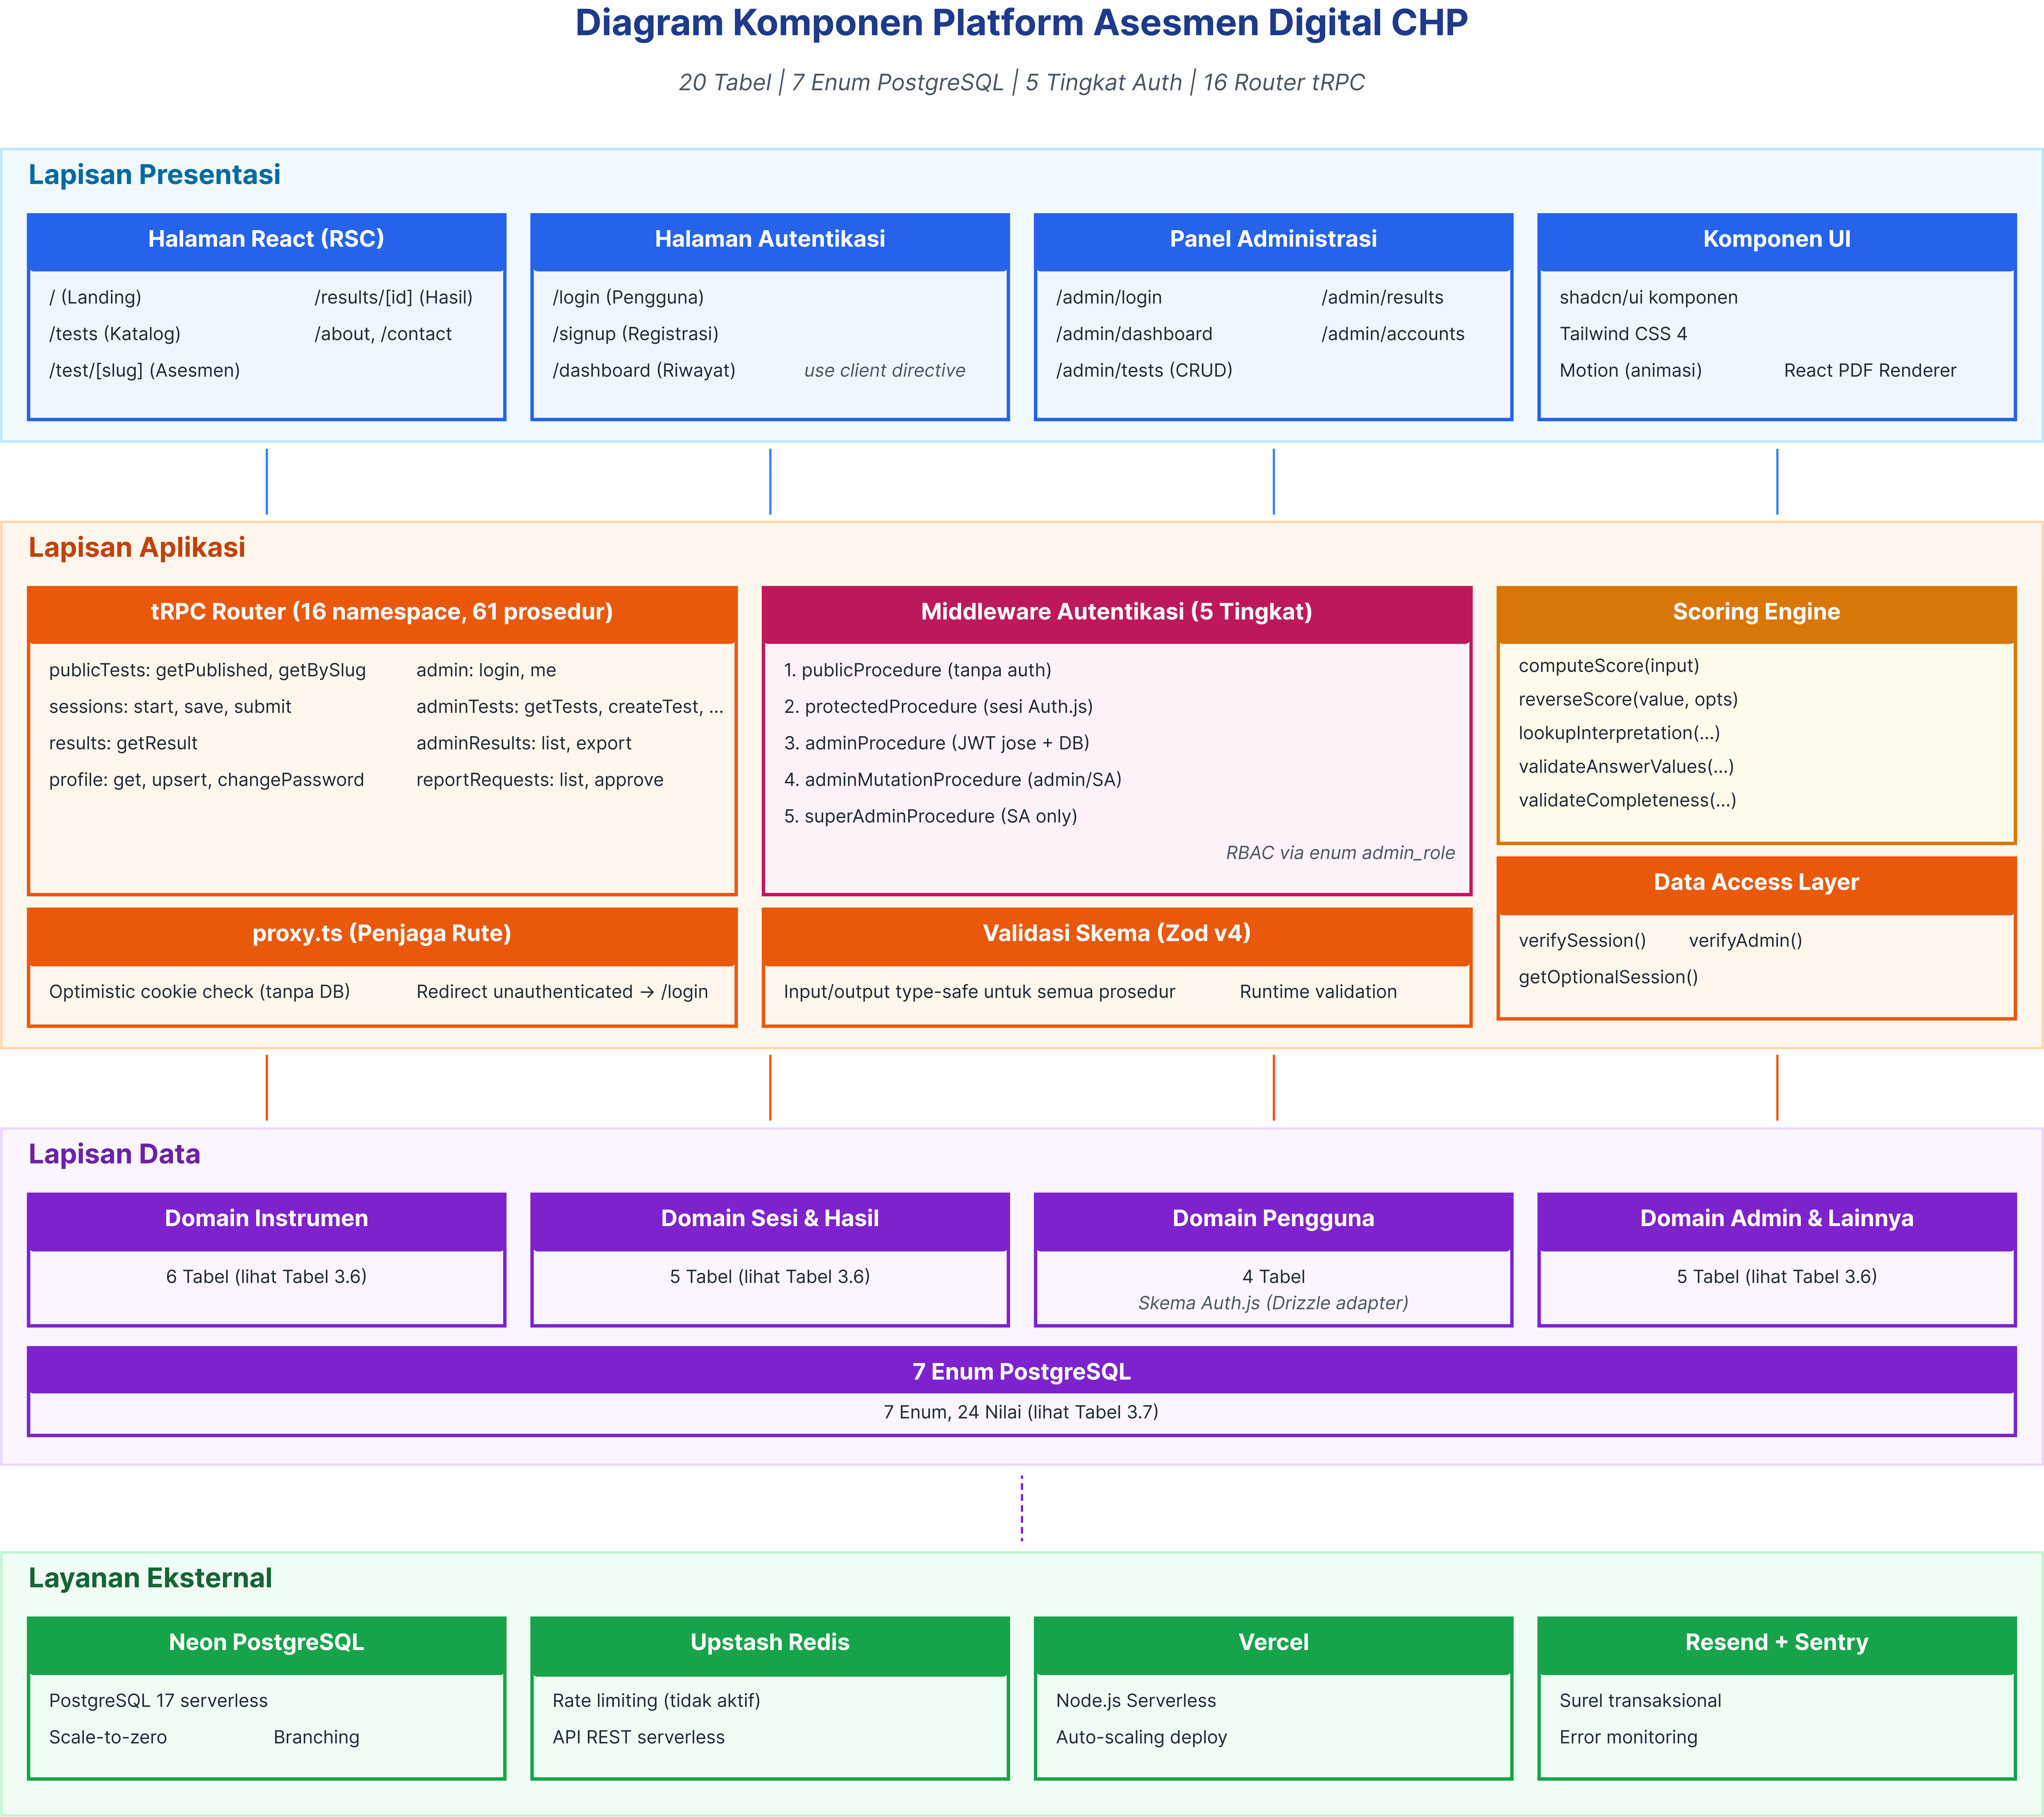
\includegraphics[width=\textwidth]{figures/gambar_3_2_komponen.png}
  \caption{Diagram Komponen Platform Asesmen Digital CHP}
  \label{fig:komponen}
\end{figure}

% [C9] Applied: 5 auth tiers in middleware description
Lapisan aplikasi terdiri atas empat modul utama:

\begin{enumerate}[leftmargin=2cm]
  \item \textit{Router} tRPC (16 \textit{namespace}) yang mengekspos 69 prosedur API.
  \item \textit{Scoring engine} (\texttt{computeScore}, \texttt{reverseScore}, \texttt{lookupInterpretation}, \texttt{validateAnswerValues}, \texttt{validateCompleteness}) yang mengandung logika komputasi skor deterministik.
  \item \textit{Middleware} autentikasi yang menerapkan lima tingkat kontrol akses: \texttt{publicProcedure}, \texttt{protectedProcedure}, \texttt{adminProcedure}, \texttt{adminMutationProcedure}, dan \texttt{superAdminProcedure}.
  \item \textit{Data Access Layer} (DAL) yang menyediakan fungsi \texttt{verifySession}, \texttt{verifyAdmin}, dan \texttt{getOptionalSession}.
\end{enumerate}

\subsection{Batas Klien-\textit{Server}}
\label{subsec:batas-klien-server}

% [C10] Applied: proxy.ts, not middleware.ts
Modul \texttt{proxy.ts} (pengganti \texttt{middleware.ts} pada Next.js 16) berfungsi sebagai penjaga rute optimistis yang membaca \textit{cookie} sesi tanpa mengakses basis data. Pemeriksaan otorisasi definitif dilakukan oleh DAL di lapisan aplikasi, sehingga keamanan bergantung pada dua lapis pertahanan yang saling menguatkan.

% ─────────────────────────────────────────────────────────────────────────────
% [C1] Applied: 16 → 20 tables; [C7] Applied: 4 missing tables added
\section{Perancangan Basis Data}
\label{sec:perancangan-db}

Skema basis data Platform CHP dirancang dengan tiga prinsip utama: (1) fleksibilitas untuk beragam instrumen psikologi; (2) pemisahan data kesehatan dari data identitas pribadi; dan (3) reproduktibilitas ilmiah melalui penyimpanan versi instrumen dan algoritma.

\subsection{Model Domain}

Skema basis data diorganisasi ke dalam lima domain:

\begin{enumerate}[leftmargin=2cm]
  \item \textbf{Domain Instrumen Asesmen} (6 tabel): mendefinisikan struktur instrumen psikometri.
  \item \textbf{Domain Sesi dan Hasil} (5 tabel): mencatat pelaksanaan asesmen.
  \item \textbf{Domain Pengguna} (4 tabel): menyediakan infrastruktur identitas dan profil.
  \item \textbf{Domain Admin dan Audit} (2 tabel): mendefinisikan pengguna administratif dan jejak audit.
  \item \textbf{Domain Permintaan dan Surel} (2 tabel): mengelola permintaan laporan dan PII.
  \item \textbf{Domain Infrastruktur Autentikasi} (1 tabel): \textit{token} verifikasi.
\end{enumerate}

\subsection{Skema Tabel}

Seluruh tabel menggunakan UUID v4 sebagai kunci primer. Tabel~\ref{tab:inventaris-tabel} menyajikan inventaris lengkap 20 tabel.

\begin{longtable}{@{}p{2.5cm} p{3cm} p{3.5cm} p{5cm}@{}}
  \caption{Inventaris Tabel Basis Data Platform CHP}
  \label{tab:inventaris-tabel} \\
  \toprule
  \textbf{Domain} & \textbf{Tabel} & \textbf{Kolom Kunci} & \textbf{Tujuan} \\
  \midrule
  \endfirsthead
  \toprule
  \textbf{Domain} & \textbf{Tabel} & \textbf{Kolom Kunci} & \textbf{Tujuan} \\
  \midrule
  \endhead
  \bottomrule
  \endfoot
  Instrumen & \texttt{tests} & id, slug, title, version & Metadata instrumen psikometri \\[0.2em]
  Instrumen & \texttt{questions} & id, test\_id, type, dimension & Butir soal dengan dimensi dan pembobotan \\[0.2em]
  Instrumen & \texttt{options} & id, question\_id, label, value & Opsi jawaban per butir soal \\[0.2em]
  Instrumen & \texttt{scoring\_rules} & id, test\_id, algorithm, config & Konfigurasi algoritma penilaian \\[0.2em]
  Instrumen & \texttt{result\_interpretations} & id, test\_id, dimension, min/max\_score & Pemetaan skor ke label interpretasi \\[0.2em]
  Instrumen & \texttt{test\_citations} & id, test\_id, type, citation, doi & Sitasi akademik per instrumen \\[0.2em]
  \midrule
  Sesi & \texttt{test\_sessions} & id, test\_id, status, claim\_token & Sesi asesmen dengan mekanisme klaim \\[0.2em]
  Sesi & \texttt{answers} & id, session\_id, question\_id, value & Respons mentah yang \textit{immutable} \\[0.2em]
  Sesi & \texttt{results} & id, session\_id, total\_score, dimension\_scores & Skor terhitung terpisah dari respons mentah \\[0.2em]
  Sesi & \texttt{session\_demographics} & session\_id, name, sex, age, province & Data demografis peserta per sesi \\[0.2em]
  Sesi & \texttt{consents} & id, session\_id, tos\_accepted, consent\_version & Persetujuan eksplisit sesuai UU PDP \\[0.2em]
  \midrule
  Pengguna & \texttt{users} & id, email, password\_hash, role & Identitas pengguna terdaftar \\[0.2em]
  Pengguna & \texttt{user\_profiles} & user\_id, display\_name, sex, age & Profil pengguna yang diperluas \\[0.2em]
  Pengguna & \texttt{accounts} & id, user\_id, provider & Tautan akun OAuth pihak ketiga \\[0.2em]
  Pengguna & \texttt{auth\_sessions} & id, session\_token, user\_id, expires & Sesi autentikasi berbasis basis data \\[0.2em]
  \midrule
  Admin & \texttt{admin\_users} & id, email, role, is\_active & Pengguna administratif dengan peran \\[0.2em]
  Admin & \texttt{audit\_logs} & id, admin\_user\_id, action, entity\_type & Jejak audit \textit{append-only} \\[0.2em]
  \midrule
  Permintaan & \texttt{report\_requests} & id, session\_id, status, requester\_type & Permintaan laporan dengan alur persetujuan \\[0.2em]
  Permintaan & \texttt{guest\_leads} & id, session\_id, encrypted\_email & PII terenkripsi AES-256-GCM \\[0.2em]
  \midrule
  Auth & \texttt{verification\_tokens} & identifier, token, expires & \textit{Token} verifikasi sekali pakai \\
\end{longtable}

Selain 20 tabel, skema mendefinisikan tujuh \textit{enum} PostgreSQL yang memastikan integritas data. Tabel~\ref{tab:enum-postgresql} mencantumkan definisinya.

\begin{table}[htbp]
  \centering
  \caption{Definisi \textit{Enum} PostgreSQL}
  \label{tab:enum-postgresql}
  \begin{tabularx}{\textwidth}{@{}l X l@{}}
    \toprule
    \textbf{Nama Enum} & \textbf{Nilai yang Diizinkan} & \textbf{Digunakan Pada} \\
    \midrule
    \texttt{test\_status} & \texttt{draft}, \texttt{published}, \texttt{archived} & \texttt{tests.status} \\
    \texttt{scoring\_method} & \texttt{summative}, \texttt{dimensional}, \texttt{binary\_cluster} & \texttt{tests.scoring\_method} \\
    \texttt{question\_type} & \texttt{likert\_5}, \texttt{likert\_7}, \texttt{multiple\_choice}, \texttt{slider}, \texttt{multi\_select} & \texttt{questions.type} \\
    \texttt{scoring\_algorithm} & \texttt{summative}, \texttt{weighted}, \texttt{reversed}, \texttt{dimensional}, \texttt{percentile} & \texttt{scoring\_rules.algorithm} \\
    \texttt{severity\_level} & \texttt{low}, \texttt{moderate}, \texttt{high}, \texttt{critical} & \texttt{result\_interpretations.severity} \\
    \texttt{session\_status} & \texttt{in\_progress}, \texttt{completed}, \texttt{abandoned} & \texttt{test\_sessions.status} \\
    \texttt{admin\_role} & \texttt{super\_admin}, \texttt{admin}, \texttt{psychiatrist}, \texttt{researcher} & \texttt{admin\_users.role} \\
    \bottomrule
  \end{tabularx}
\end{table}

\subsection{Relasi Antar-Entitas}

Gambar~\ref{fig:er-diagram} menyajikan diagram \textit{Entity-Relationship} (ER).

\begin{figure}[htbp]
  \centering
  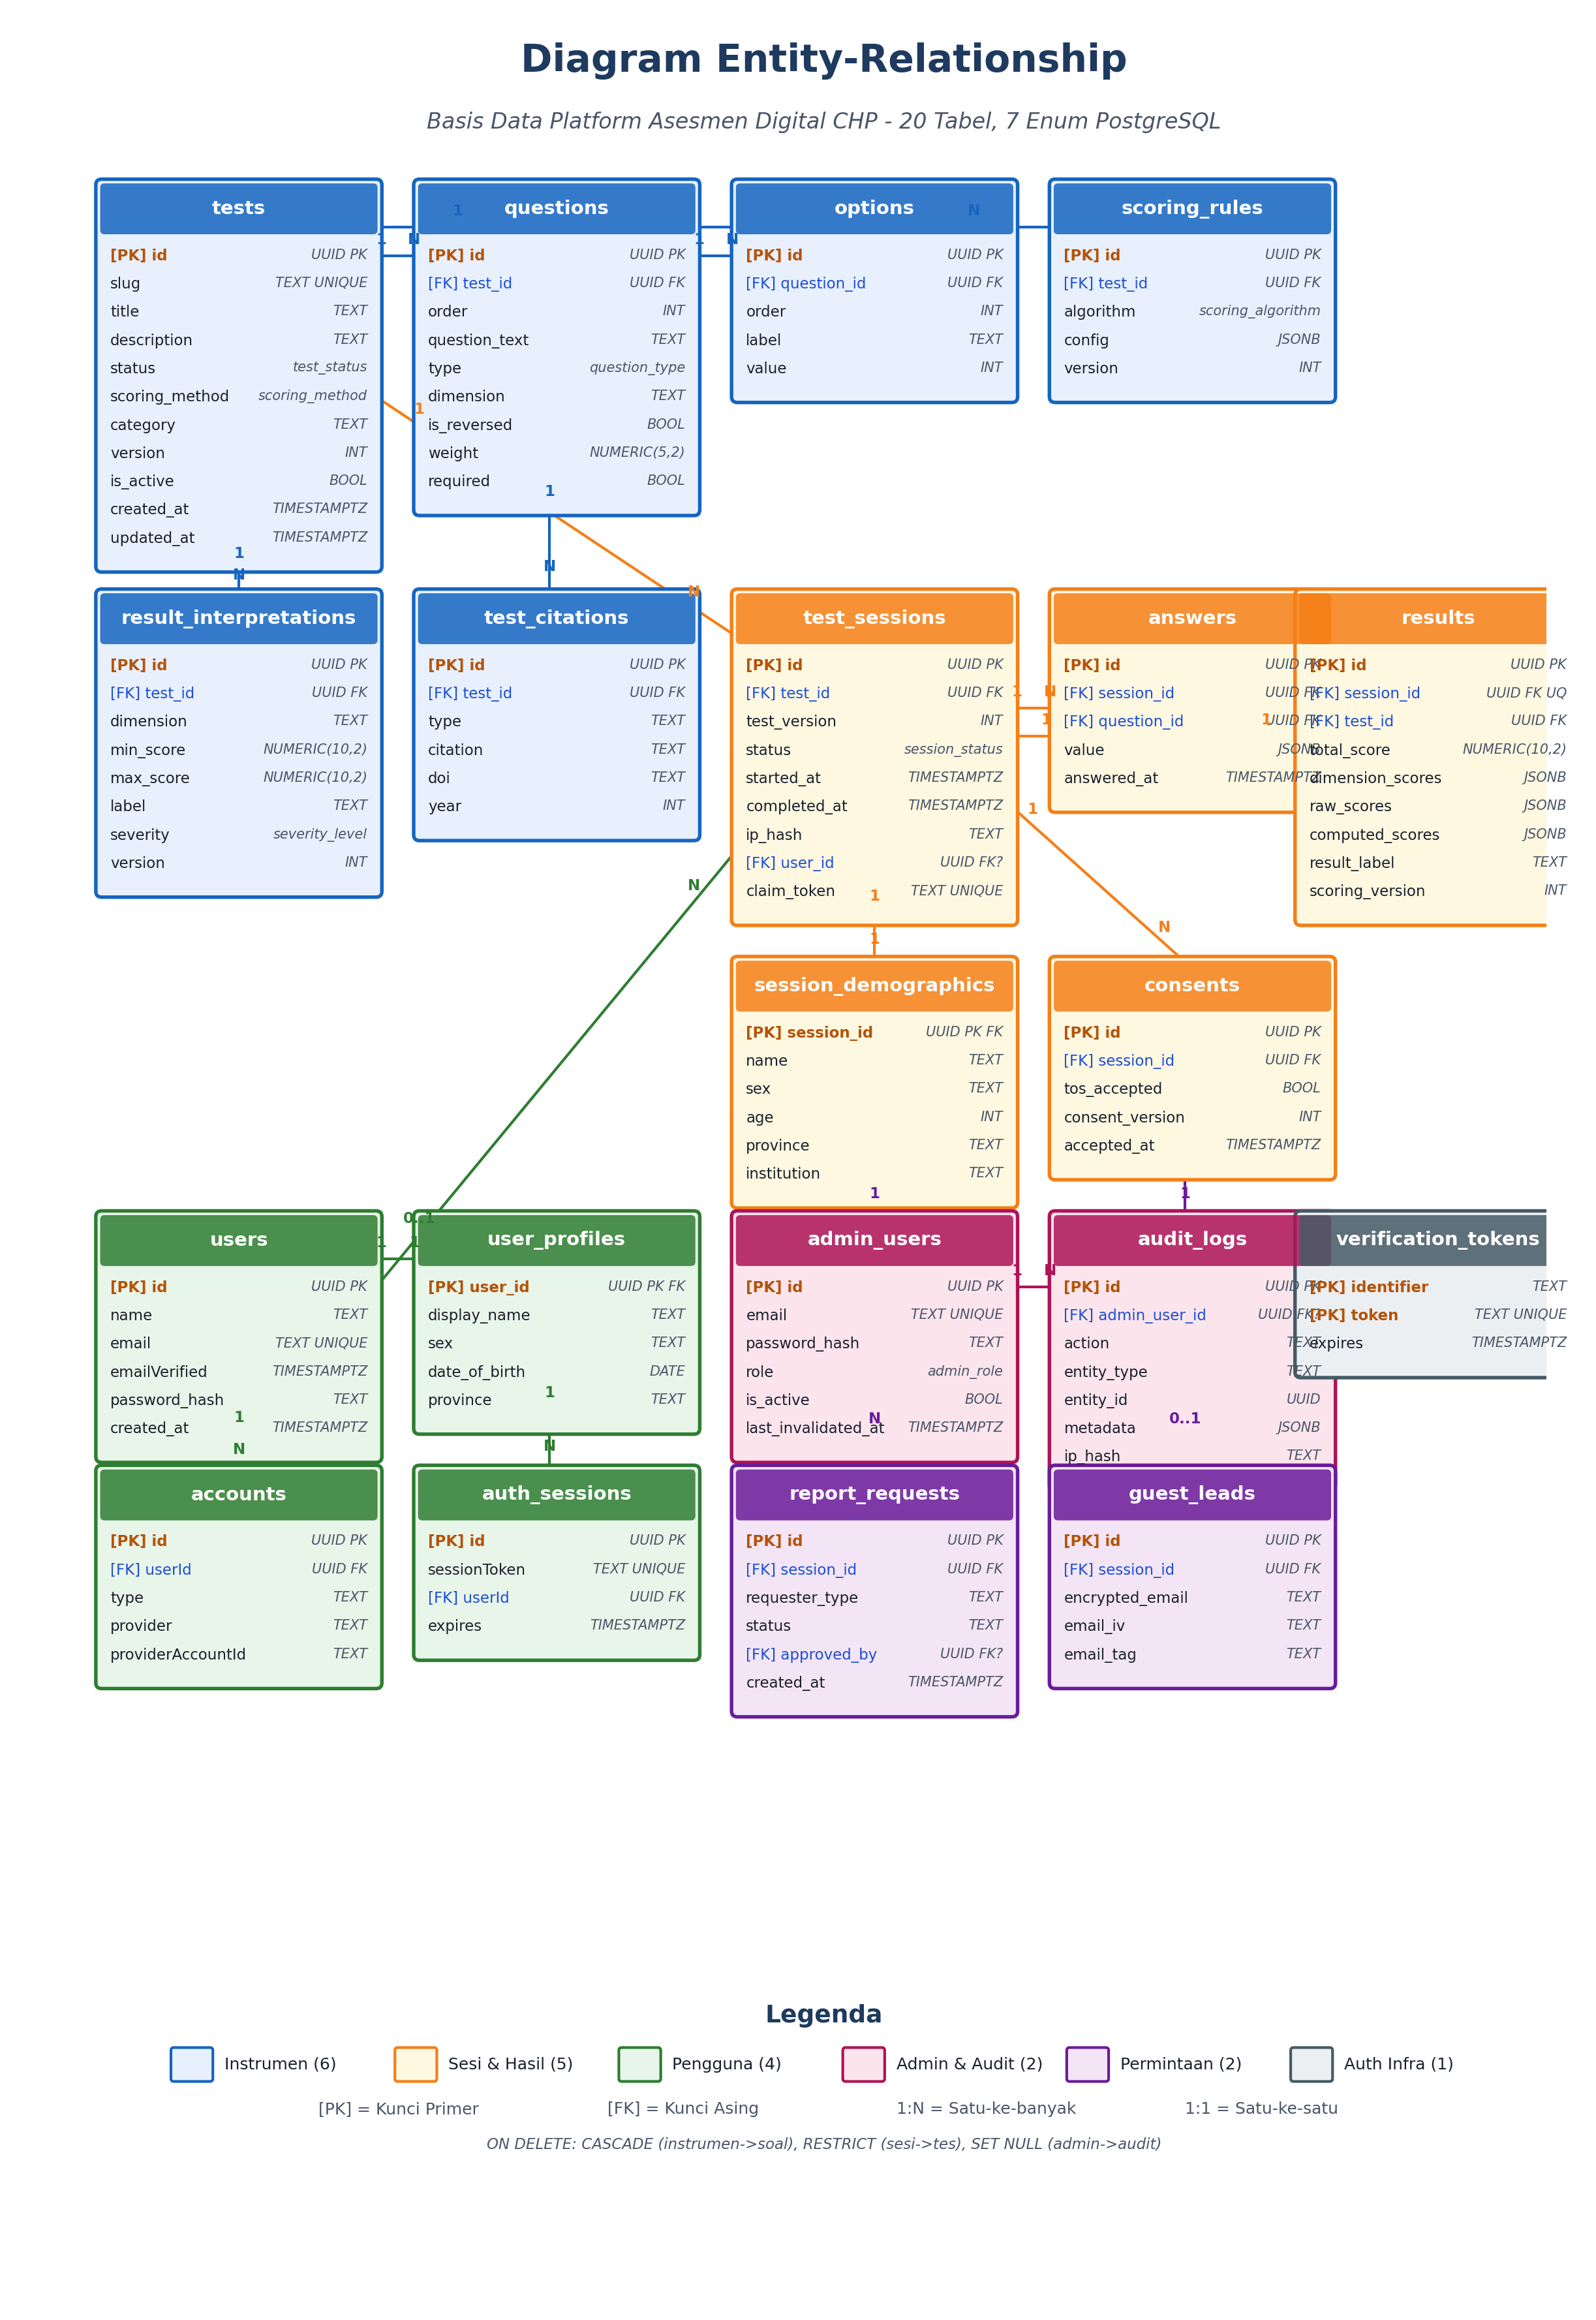
\includegraphics[width=\textwidth]{figures/gambar_3_3_er_diagram.png}
  \caption{Diagram \textit{Entity-Relationship} Basis Data Platform CHP}
  \label{fig:er-diagram}
\end{figure}

Relasi utama antar-entitas:

\begin{enumerate}[leftmargin=2cm]
  \item \texttt{tests} $\rightarrow$ \texttt{questions} $\rightarrow$ \texttt{options}: pola satu-ke-banyak bertingkat dengan \texttt{ON DELETE CASCADE}.
  \item \texttt{test\_sessions} $\rightarrow$ \texttt{answers}: \textit{constraint} unik komposit \texttt{(session\_id, question\_id)}.
  \item \texttt{test\_sessions} $\rightarrow$ \texttt{results}: relasi satu-ke-satu melalui \textit{constraint} \texttt{UNIQUE} pada \texttt{session\_id}.
  \item \texttt{test\_sessions} $\rightarrow$ \texttt{users}: \textit{foreign key} opsional (\texttt{user\_id} \textit{nullable}) dengan \texttt{ON DELETE SET NULL}.
  \item \texttt{admin\_users} $\rightarrow$ \texttt{audit\_logs}: \texttt{ON DELETE SET NULL} agar penghapusan akun admin tidak menghapus rekam jejak.
\end{enumerate}

\subsection{Keputusan Perancangan Kritis}

Empat keputusan perancangan data dengan dampak arsitektur signifikan:

\begin{enumerate}[leftmargin=2cm]
  \item \textbf{Pemisahan \texttt{answers} dan \texttt{results}}: memungkinkan \textit{re-scoring} tanpa kehilangan data historis.
  \item \textbf{JSONB untuk nilai polimorfik}: kolom \texttt{answers.value} mengakomodasi format jawaban beragam (Likert, pilihan ganda, \textit{slider}).
  \item \textbf{\textit{Claim token}}: UUID v4 dengan masa berlaku 72 jam untuk transisi anonim-ke-terdaftar; sekali pakai dan dinihilkan setelah diklaim.
  \item \textbf{Penyamaran IP dan enkripsi surel}: alamat IP di-\textit{hash} satu arah; surel dienkripsi AES-256-GCM dalam tabel \texttt{guest\_leads} yang terisolasi.
\end{enumerate}

% ─────────────────────────────────────────────────────────────────────────────
% [C3/C8] REWRITTEN: API table expanded from 8 to 22 key procedures
\section{Perancangan Antarmuka Pemrograman Aplikasi}
\label{sec:perancangan-api}

Platform CHP menggunakan tRPC sebagai protokol komunikasi. Seluruh 69 prosedur API diorganisasi ke dalam 16 \textit{router namespace}. Tabel~\ref{tab:api-publik} hingga Tabel~\ref{tab:api-admin} menyajikan inventaris prosedur yang dikelompokkan berdasarkan area fungsional.

\begin{longtable}{@{}l l c c p{5cm}@{}}
  \caption{Prosedur API Publik (Alur Asesmen)}
  \label{tab:api-publik} \\
  \toprule
  \textbf{Prosedur} & \textbf{Router} & \textbf{Tipe} & \textbf{Auth} & \textbf{Fungsi} \\
  \midrule
  \endfirsthead
  \toprule
  \textbf{Prosedur} & \textbf{Router} & \textbf{Tipe} & \textbf{Auth} & \textbf{Fungsi} \\
  \midrule
  \endhead
  \bottomrule
  \endfoot
  \texttt{getPublishedTests} & publicTests & Q & Publik & Ambil daftar tes aktif \\
  \texttt{getTestBySlug} & publicTests & Q & Publik & Ambil tes berdasarkan \textit{slug} \\
  \texttt{startSession} & sessions & M & Publik & Mulai sesi, simpan \textit{consent} + \textit{claim token} \\
  \texttt{saveDemographics} & sessions & M & Publik & Simpan data demografis \\
  \texttt{saveProgress} & sessions & M & Publik & Simpan jawaban (\textit{batch upsert}) \\
  \texttt{submitAssessment} & sessions & M & Publik & Validasi, hitung skor, simpan hasil \\
  \texttt{getResult} & results & Q & Publik & Ambil hasil asesmen \\
  \texttt{requestEmailReport} & sessions & M & Publik & Buat permintaan laporan surel \\
\end{longtable}

\begin{longtable}{@{}l l c c p{5cm}@{}}
  \caption{Prosedur API Pengguna Terdaftar}
  \label{tab:api-user} \\
  \toprule
  \textbf{Prosedur} & \textbf{Router} & \textbf{Tipe} & \textbf{Auth} & \textbf{Fungsi} \\
  \midrule
  \endfirsthead
  \toprule
  \textbf{Prosedur} & \textbf{Router} & \textbf{Tipe} & \textbf{Auth} & \textbf{Fungsi} \\
  \midrule
  \endhead
  \bottomrule
  \endfoot
  \texttt{claimSession} & sessions & M & Protected & Klaim sesi anonim ke akun \\
  \texttt{get} & profile & Q & Protected & Ambil profil pengguna \\
  \texttt{upsert} & profile & M & Protected & Simpan/perbarui profil \\
  \texttt{changePassword} & profile & M & Protected & Ganti kata sandi \\
\end{longtable}

\begin{longtable}{@{}l l c c p{5cm}@{}}
  \caption{Prosedur API Panel Administrasi}
  \label{tab:api-admin} \\
  \toprule
  \textbf{Prosedur} & \textbf{Router} & \textbf{Tipe} & \textbf{Auth} & \textbf{Fungsi} \\
  \midrule
  \endfirsthead
  \toprule
  \textbf{Prosedur} & \textbf{Router} & \textbf{Tipe} & \textbf{Auth} & \textbf{Fungsi} \\
  \midrule
  \endhead
  \bottomrule
  \endfoot
  \texttt{login} & admin & M & Publik & \textit{Login} admin, terbitkan JWT \\
  \texttt{me} & admin & Q & Admin & Profil admin aktif \\
  \texttt{stats} & adminDashboard & Q & Admin & Statistik platform \\
  \texttt{list} & adminResults & Q & Admin & Tabel hasil per instrumen \\
  \texttt{export} & adminResults & Q & Admin & Ekspor data (maks 5000 baris) \\
  \texttt{list} & reportRequests & Q & Admin & Daftar permintaan laporan \\
  \texttt{approve} & reportRequests & M & Admin & \textit{Generate} PDF + kirim surel \\
  \texttt{getTests} & adminTests & Q & Admin & Daftar instrumen \\
  \texttt{createTest} & adminTests & M & AdminMut & Buat tes baru \\
  \texttt{createAdmin} & adminAccounts & M & SuperAdmin & Buat akun admin \\
\end{longtable}

% [C9] Applied in middleware description
Setiap prosedur memanfaatkan lima tingkat \textit{middleware} autentikasi: \texttt{publicProcedure} (tanpa autentikasi), \texttt{protectedProcedure} (sesi Auth.js), \texttt{adminProcedure} (JWT admin via jose dengan validasi basis data), \texttt{adminMutationProcedure} (peran \texttt{super\_admin} atau \texttt{admin}), dan \texttt{superAdminProcedure} (khusus \texttt{super\_admin}).

% ─────────────────────────────────────────────────────────────────────────────
\section{Perancangan Alur Antarmuka Pengguna}
\label{sec:alur-ui}

Perancangan komponen antarmuka pengguna secara visual merupakan tanggung jawab anggota tim lain. Namun, perancangan alur layar (\textit{screen flow}) merupakan bagian integral dari arsitektur sistem.

\begin{figure}[htbp]
  \centering
  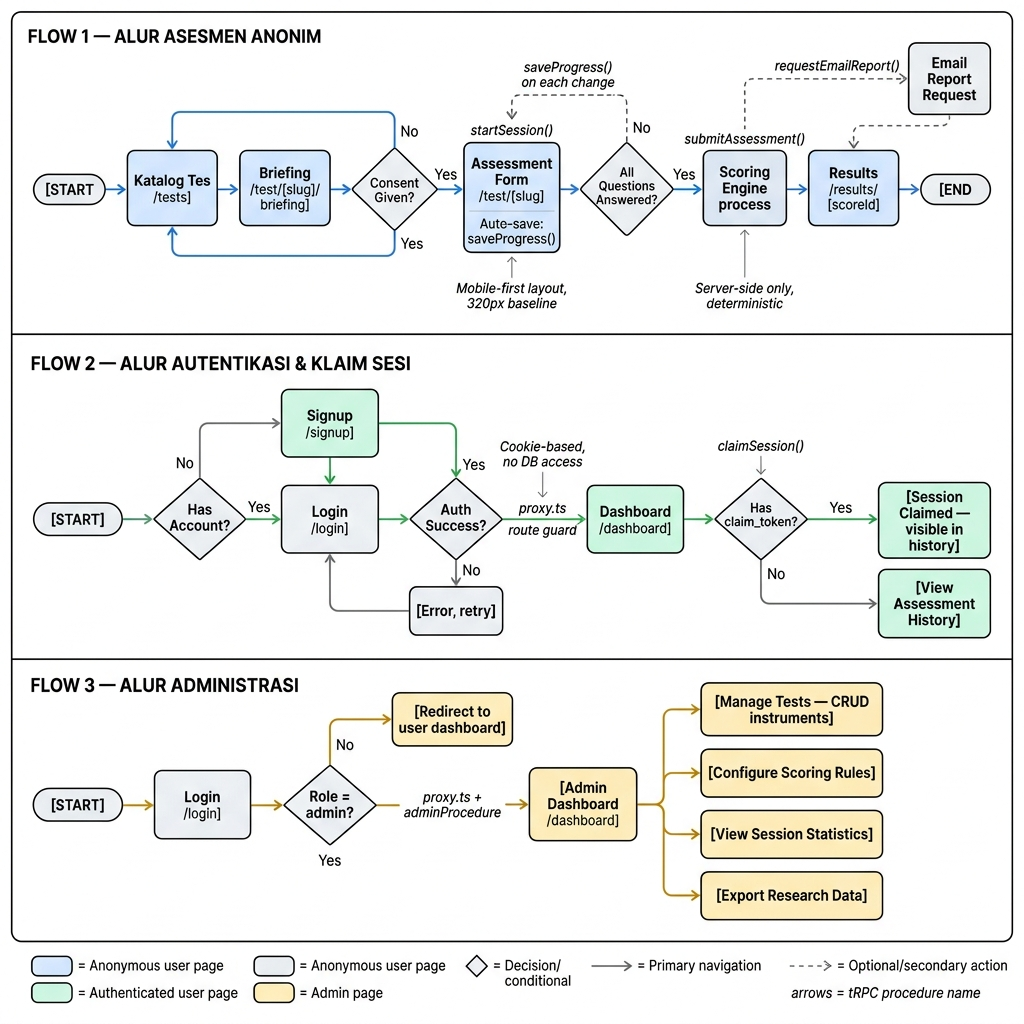
\includegraphics[width=\textwidth]{figures/gambar_3_4_alur_layar.png}
  \caption{Diagram Alur Layar Platform CHP}
  \label{fig:screen-flow}
\end{figure}

Tiga alur utama:

\begin{enumerate}[leftmargin=2cm]
  \item \textbf{Alur asesmen anonim}: \texttt{/tests} $\rightarrow$ \texttt{/test/[slug]} $\rightarrow$ \texttt{/results/[scoreId]}. Seluruh alur berjalan tanpa memerlukan akun.
  \item \textbf{Alur autentikasi dan klaim sesi}: \texttt{/signup} atau \texttt{/login} $\rightarrow$ \texttt{/dashboard}. Penjaga rute \texttt{proxy.ts} memastikan halaman terlindungi hanya diakses oleh pengguna terautentikasi.
  \item \textbf{Alur administrasi}: \texttt{/admin/login} $\rightarrow$ \texttt{/admin/dashboard} $\rightarrow$ halaman manajemen instrumen, hasil, laporan, dan akun.
\end{enumerate}


% ── BAB IV: Implementasi dan Testing ────────────────────────────────────────
% =============================================================================
% 40-bab4.tex — BAB IV IMPLEMENTASI DAN TESTING
% =============================================================================
\chapter{IMPLEMENTASI DAN TESTING}
\label{chap:implementasi}

Bab ini memaparkan implementasi sistem berdasarkan perancangan yang telah diuraikan pada Bab~\ref{chap:analisa-perancangan}. Pembahasan mencakup lingkungan pengembangan, implementasi basis data, \textit{scoring engine}, API tRPC, sistem autentikasi, panel administrasi, generasi PDF dan pengiriman surel, pengujian unit, \textit{pipeline} CI/CD, serta \textit{deployment} ke lingkungan produksi.

% ─────────────────────────────────────────────────────────────────────────────
\section{Lingkungan Pengembangan}
\label{sec:lingkungan-dev}

Pengembangan Platform CHP dilakukan pada lingkungan lokal dengan spesifikasi perangkat lunak yang tercantum pada Tabel~\ref{tab:kebutuhan-software}. Manajer paket yang digunakan adalah pnpm versi 9, yang dipilih karena efisiensi penyimpanannya melalui mekanisme \textit{content-addressable store} yang menghindari duplikasi dependensi antar proyek.

Konfigurasi TypeScript menggunakan mode \texttt{strict: true} dengan opsi tambahan \texttt{noUncheckedIndexedAccess}, \texttt{noUnusedLocals}, dan \texttt{noUnusedParameters} untuk memaksimalkan deteksi kesalahan pada waktu kompilasi. Tiga \textit{path alias} dikonfigurasi untuk menyederhanakan impor modul: \texttt{@/*} untuk direktori \texttt{src/}, \texttt{@/server/*} untuk \texttt{src/server/}, dan \texttt{@/components/*} untuk \texttt{src/components/}.

Seluruh \textit{environment variable} yang diperlukan didokumentasikan dalam \textit{file} \texttt{.env.example} yang berisi 16 variabel konfigurasi, mencakup koneksi basis data (\texttt{DATABASE\_URL}), kunci autentikasi (\texttt{AUTH\_SECRET}, \texttt{ADMIN\_JWT\_SECRET}), konfigurasi layanan pihak ketiga (Upstash Redis, Sentry, Resend), dan kunci enkripsi (\texttt{ENCRYPTION\_KEY} sepanjang 64 karakter heksadesimal untuk AES-256-GCM).

% ─────────────────────────────────────────────────────────────────────────────
\section{Implementasi Basis Data}
\label{sec:impl-database}

Skema basis data yang dirancang pada Subbab~\ref{sec:perancangan-db} diimplementasikan menggunakan Drizzle ORM versi 1.0.0-beta.20 dengan \textit{driver} Neon HTTP (\texttt{@neondatabase/serverless}). Definisi skema diorganisasi ke dalam 14 \textit{file} TypeScript di dalam direktori \texttt{src/server/schema/}, dengan setiap \textit{file} bertanggung jawab atas satu domain.

Seluruh 20 tabel dan 7 \textit{enum} PostgreSQL berhasil di-\textit{deploy} ke lingkungan produksi Neon PostgreSQL. Migrasi skema dikelola melalui Drizzle Kit (\texttt{drizzle-kit}) yang menghasilkan \textit{file} SQL migrasi secara otomatis berdasarkan perubahan pada definisi skema TypeScript. Pendekatan ini memastikan bahwa setiap perubahan skema terdokumentasi dan dapat direproduksi.

Relasi antar-tabel diimplementasikan menggunakan \texttt{defineRelations()} dari Drizzle ORM v2, yang memisahkan definisi relasi dari definisi kolom. Pola ini memungkinkan kueri relasional (\textit{relational queries}) yang menghasilkan SQL \texttt{JOIN} secara otomatis tanpa memerlukan penulisan kueri manual.

Data awal (\textit{seed data}) untuk empat instrumen psikometri---PSS-10, GPIUS-2, SRS, dan SRQ-29---disiapkan melalui skrip \textit{seeding} yang memasukkan definisi tes, butir soal, opsi jawaban, dan rentang interpretasi. Skrip ini memastikan lingkungan pengembangan baru dapat langsung memiliki data yang cukup untuk pengujian.

% ─────────────────────────────────────────────────────────────────────────────
\section{Implementasi \textit{Scoring Engine}}
\label{sec:impl-scoring}

\textit{Scoring engine} diimplementasikan sebagai \textit{pipeline} fungsi murni (\textit{pure functions}) dalam tiga \textit{file} di direktori \texttt{src/server/scoring/}. Desain ini menjamin determinisme: untuk masukan yang sama, keluaran selalu identik, tanpa efek samping (\textit{side effects}) atau ketergantungan pada status eksternal.

\subsection{Fungsi \texttt{reverseScore}}

Fungsi \texttt{reverseScore(rawValue, options)} mengimplementasikan pembalikan skor secara agnostik skala menggunakan rumus:

\begin{equation}
  \text{reversedScore} = (\text{scaleMax} - \text{rawValue}) + \text{scaleMin}
\end{equation}

\noindent di mana \texttt{scaleMax} dan \texttt{scaleMin} diturunkan secara otomatis dari larik opsi yang diberikan. Pendekatan ini menghilangkan kebutuhan untuk mengonfigurasi batas skala secara manual, sehingga fungsi dapat digunakan untuk skala Likert dengan rentang apapun.

\subsection{Fungsi \texttt{computeScore}}

Fungsi \texttt{computeScore(input)} adalah inti dari \textit{scoring engine}. Fungsi ini menerima masukan berupa jawaban peserta beserta metadata soal, dan menghasilkan objek hasil yang mencakup:

\begin{enumerate}[leftmargin=2cm]
  \item Skor total (\texttt{totalScore}): penjumlahan seluruh skor butir soal setelah pembalikan dan pembobotan.
  \item Skor per dimensi (\texttt{dimensionScores}): pengelompokan skor berdasarkan kolom \texttt{dimension} pada setiap butir soal.
  \item Skor mentah per butir soal (\texttt{rawScores}): skor sebelum pembalikan untuk keperluan audit.
  \item Skor terhitung per butir soal (\texttt{computedScores}): skor setelah pembalikan dan pembobotan.
  \item Skor maksimum yang mungkin (\texttt{maxPossibleScore}): dihitung berdasarkan bobot dan opsi tertinggi.
\end{enumerate}

Untuk instrumen GPIUS-2 yang menggunakan metode \textit{Deficient Self-Regulation} (DSR), \texttt{computeScore} mengimplementasikan \textit{rollup} orde kedua: setelah menghitung skor per subskala, skor total dihitung sebagai penjumlahan subskala DSR yang merupakan gabungan dari beberapa dimensi primer.

\subsection{Fungsi \texttt{lookupInterpretation}}

Fungsi \texttt{lookupInterpretation(testId, totalScore, dimension?)} mengkueri tabel \texttt{result\_interpretations} untuk memetakan skor numerik ke label interpretasi yang dapat dibaca manusia. Fungsi ini mengembalikan label, deskripsi, rekomendasi, dan tingkat keparahan (\textit{severity level}). Pada kasus di mana tidak ditemukan rentang yang sesuai (\textit{interpretation miss}), fungsi mencatat peringatan ke Sentry tanpa melempar kesalahan, sehingga hasil asesmen tetap tersedia meskipun tanpa interpretasi.

\subsection{Fungsi Validasi}

Dua fungsi validasi---\texttt{validateAnswerValues} dan \texttt{validateCompleteness}---memastikan integritas data sebelum proses komputasi skor dimulai. Kedua fungsi bersifat murni (tanpa akses basis data), sehingga dapat diuji secara terisolasi. \texttt{validateAnswerValues} memeriksa bahwa setiap nilai jawaban berada dalam rentang opsi yang valid, sedangkan \texttt{validateCompleteness} memastikan semua butir soal wajib telah dijawab.

\subsection{Instrumen yang Diimplementasikan}

Empat instrumen psikometri berhasil dikonfigurasi dan divalidasi pada platform:

\begin{enumerate}[leftmargin=2cm]
  \item \textbf{PSS-10} (\textit{Perceived Stress Scale}): 10 butir soal, skala Likert 0--4, unidimensional, dengan 4 butir soal terbalik.
  \item \textbf{GPIUS-2} (\textit{Generalized Problematic Internet Use Scale}): 15 butir soal, skala Likert 1--5, 5 subskala dengan \textit{rollup} DSR orde kedua.
  \item \textbf{SRS} (\textit{Stress Response Scale}): 11 butir soal, skala Likert 1--6, 3 subskala.
  \item \textbf{SRQ-29} (\textit{Self-Reporting Questionnaire}): 29 butir soal, jawaban biner (Ya/Tidak), 4 kluster diagnostik.
\end{enumerate}

% ─────────────────────────────────────────────────────────────────────────────
\section{Implementasi API tRPC}
\label{sec:impl-trpc}

Seluruh 69 prosedur tRPC diimplementasikan dalam 17 \textit{file} prosedur yang diorganisasi ke dalam 16 \textit{router namespace}. Setiap prosedur mendefinisikan skema masukan menggunakan Zod dan dihubungkan ke salah satu dari lima tingkat \textit{middleware} autentikasi.

\subsection{Komposisi \textit{Router}}

\textit{File} \texttt{src/server/trpc/router.ts} berfungsi sebagai \textit{barrel file} yang mengomposisikan seluruh \textit{router} menjadi satu \textit{app router}. \textit{Router} dikelompokkan berdasarkan domain: \textit{router} publik (\texttt{publicTests}, \texttt{sessions}, \texttt{results}, \texttt{health}), \textit{router} pengguna (\texttt{profile}), dan \textit{router} admin (\texttt{admin}, \texttt{adminDashboard}, \texttt{adminTests}, \texttt{adminQuestions}, \texttt{adminScales}, \texttt{adminResults}, \texttt{reportRequests}, \texttt{adminAccounts}, \texttt{adminUserAccounts}, \texttt{adminAudit}, \texttt{adminProfile}).

\subsection{\textit{Structural Lock}}

Fitur keamanan data yang krusial pada prosedur admin adalah mekanisme \textit{structural lock}. Ketika sebuah instrumen tes telah memiliki sesi asesmen yang tercatat (diperiksa melalui fungsi \texttt{getSessionCount}), prosedur \texttt{updateTest}, \texttt{updateQuestion}, \texttt{deleteQuestion}, \texttt{reorderQuestions}, dan \texttt{updateRange} memblokir perubahan pada kolom yang sensitif terhadap penilaian---seperti \texttt{slug}, \texttt{scoringMethod}, bobot soal (\texttt{weight}), dan nilai opsi (\texttt{value}). Mekanisme ini mencegah invalidasi retroaktif terhadap data riset yang telah terkumpul.

\subsection{Operasi Idempoten}

Prosedur \texttt{saveProgress} menggunakan pola \texttt{ON CONFLICT ... DO UPDATE} (PostgreSQL \texttt{UPSERT}) pada \textit{constraint} unik komposit \texttt{(session\_id, question\_id)}, sehingga penyimpanan progres bersifat idempoten---pemanggilan berulang dengan data yang sama menghasilkan efek yang identik. Pendekatan ini menangani dengan aman skenario koneksi terputus di mana klien mungkin mengirim ulang jawaban yang sama.

% ─────────────────────────────────────────────────────────────────────────────
\section{Implementasi Autentikasi}
\label{sec:impl-auth}

Sistem autentikasi diimplementasikan sebagai dua subsistem yang sepenuhnya terpisah, masing-masing dengan mekanisme \textit{token}, penyimpanan \textit{cookie}, dan siklus hidup sesi yang independen.

\subsection{Autentikasi Pengguna Publik (Auth.js v5)}

Auth.js (NextAuth v5, versi 5.0.0-beta.30) digunakan untuk autentikasi pengguna publik dengan konfigurasi berikut:

\begin{enumerate}[leftmargin=2cm]
  \item \textbf{Strategi sesi}: JWT (\texttt{session: \{ strategy: "jwt" \}}).
  \item \textbf{\textit{Provider}}: \texttt{CredentialsProvider} dengan validasi surel dan kata sandi.
  \item \textbf{\textit{Password hashing}}: bcryptjs dengan \textit{cost factor} 12.
  \item \textbf{Adaptor}: \texttt{CHPDrizzleAdapter} kustom yang dipersiapkan untuk integrasi OAuth di masa mendatang.
  \item \textbf{\textit{Callbacks}}: \textit{callback} JWT menanamkan \texttt{userId} dan \texttt{role} ke dalam \textit{token}; \textit{callback} \texttt{session} meneruskan informasi ini ke konteks sesi.
\end{enumerate}

\subsection{Autentikasi Administrator (jose JWT)}

Subsistem autentikasi admin diimplementasikan secara mandiri menggunakan pustaka jose tanpa ketergantungan pada Auth.js:

\begin{enumerate}[leftmargin=2cm]
  \item \textbf{Algoritma}: HS256 dengan kunci rahasia \texttt{ADMIN\_JWT\_SECRET} (minimal 32 karakter).
  \item \textbf{\textit{Sliding window}}: setiap permintaan admin yang valid memperpanjang masa berlaku \textit{token} 30 menit dari waktu saat ini.
  \item \textbf{Batas keras}: \textit{token} tidak dapat diperpanjang melebihi 8 jam dari waktu penerbitan awal (\texttt{originalIat}), memaksa \textit{login} ulang untuk sesi yang sangat panjang.
  \item \textbf{Penyimpanan}: JWT disimpan dalam \textit{cookie} bernama \texttt{admin-token}, dikelola melalui modul \texttt{cookies.ts} yang menggunakan \texttt{ctx.resHeaders} (bukan \texttt{cookies()}) untuk kompatibilitas dengan konteks tRPC.
  \item \textbf{Revokasi}: prosedur \texttt{logout} menetapkan kolom \texttt{sessionInvalidatedAt} di basis data sebelum menghapus \textit{cookie}. \textit{Middleware} \texttt{adminProcedure} memeriksa kolom ini pada setiap permintaan, sehingga \textit{token} yang dicuri setelah \textit{logout} tidak dapat digunakan.
\end{enumerate}

\subsection{\textit{Rate Limiting} pada \textit{Login} Admin}

Modul \texttt{rate-limiter.ts} mengimplementasikan \textit{rate limiting in-memory} berlapis dua:

\begin{enumerate}[leftmargin=2cm]
  \item \textbf{Berbasis IP}: 5 kegagalan dalam jendela waktu 5 menit memicu penundaan (\textit{cooldown}) yang pulih secara otomatis setelah jendela berakhir.
  \item \textbf{Berbasis akun}: 10 kegagalan kumulatif mengunci akun secara permanen, memerlukan intervensi \texttt{super\_admin} melalui prosedur \texttt{unlockAdmin}. Mekanisme ini disimpan dalam \textit{in-memory} yang memadai untuk skala kurang dari 10 pengguna admin.
\end{enumerate}

% ─────────────────────────────────────────────────────────────────────────────
\section{Implementasi Panel Administrasi}
\label{sec:impl-admin}

Panel administrasi diakses melalui rute \texttt{/admin/(dashboard)/*} dan dilindungi oleh penjaga rute \texttt{proxy.ts} yang memeriksa keberadaan \textit{cookie} \texttt{admin-token}. Panel terdiri atas delapan modul utama:

\begin{enumerate}[leftmargin=2cm]
  \item \textbf{\textit{Dashboard}}: statistik agregat platform---jumlah asesmen selesai, sesi aktif, tingkat penyelesaian, tes terpopuler, dan hasil terbaru.
  \item \textbf{Manajemen Instrumen} (\texttt{adminTests}): CRUD tes dengan transisi status \texttt{draft} $\rightarrow$ \texttt{published} $\rightarrow$ \texttt{archived}, dilengkapi \textit{structural lock} untuk instrumen yang telah memiliki sesi.
  \item \textbf{Manajemen Soal} (\texttt{adminQuestions}): penambahan, penyuntingan, penghapusan, dan pengurutan ulang butir soal beserta opsi jawaban.
  \item \textbf{Konfigurasi Skala} (\texttt{adminScales}): pengelolaan rentang interpretasi per dimensi.
  \item \textbf{Data Hasil} (\texttt{adminResults}): tabel data dengan paginasi, filter, dan pengurutan; ekspor data dengan batas 5000 baris yang mencakup jawaban per butir soal.
  \item \textbf{Permintaan Laporan} (\texttt{reportRequests}): alur persetujuan bertahap (\textit{pending} $\rightarrow$ \textit{reviewed} $\rightarrow$ \textit{approved/rejected}) dengan dukungan persetujuan \textit{batch}.
  \item \textbf{Manajemen Akun Admin} (\texttt{adminAccounts}, khusus \texttt{super\_admin}): pembuatan akun, perubahan peran, aktivasi/deaktivasi, pembukaan kunci, dan invalidasi sesi paksa. Dilengkapi pengaman \textit{last super admin} yang mencegah penonaktifan \texttt{super\_admin} terakhir.
  \item \textbf{Jejak Audit} (\texttt{adminAudit}): log paginasi dengan filter cepat, pembatasan peran, dan resolusi label entitas. Setiap mutasi administratif menulis ke tabel \texttt{audit\_logs}.
\end{enumerate}

% ─────────────────────────────────────────────────────────────────────────────
\section{Implementasi Generasi PDF dan Pengiriman Surel}
\label{sec:impl-pdf-email}

Generasi laporan hasil asesmen menggunakan \texttt{@react-pdf/renderer} versi 4.5.1, yang memungkinkan pembuatan dokumen PDF menggunakan komponen React. Laporan yang dihasilkan mencakup informasi tes, skor total, skor per dimensi, label interpretasi, dan rekomendasi.

Pengiriman surel menggunakan layanan Resend versi 6.12.2, yang menyediakan API transaksional untuk pengiriman surel dari lingkungan \textit{serverless}. Alur lengkap---dari penerimaan permintaan melalui prosedur \texttt{approve} pada \textit{router} \texttt{reportRequests}, generasi PDF, hingga pengiriman surel---dieksekusi secara atomik dalam satu prosedur tRPC.

% ─────────────────────────────────────────────────────────────────────────────
\section{Pengujian Unit}
\label{sec:impl-unit-test}

Pengujian unit dilaksanakan menggunakan Vitest versi 4.1.5 dengan konfigurasi yang didefinisikan dalam \texttt{vitest.config.ts}. Total 235 kasus uji (\textit{test cases}) ditulis dalam 20 \textit{file} uji yang diorganisasi berdasarkan modul. Tabel~\ref{tab:inventaris-test} menyajikan inventaris lengkap.

\begin{longtable}{@{}p{6.5cm} c@{}}
  \caption{Inventaris \textit{File} Pengujian Unit}
  \label{tab:inventaris-test} \\
  \toprule
  \textbf{\textit{File} Uji} & \textbf{Jumlah Kasus Uji} \\
  \midrule
  \endfirsthead
  \toprule
  \textbf{\textit{File} Uji} & \textbf{Jumlah Kasus Uji} \\
  \midrule
  \endhead
  \bottomrule
  \endfoot
  \texttt{scoring/engine.test.ts} & $\sim$25 \\
  \texttt{scoring/reverseScore.test.ts} & $\sim$26 \\
  \texttt{scoring/validation.test.ts} & $\sim$21 \\
  \texttt{data/interpretations.test.ts} & $\sim$44 \\
  \texttt{data/srq29-questions.test.ts} & $\sim$8 \\
  \texttt{admin-questions/admin-questions.test.ts} & $\sim$18 \\
  \texttt{admin-accounts/admin-accounts.test.ts} & $\sim$16 \\
  \texttt{admin-scales/admin-scales.test.ts} & $\sim$12 \\
  \texttt{encryption.test.ts} & $\sim$12 \\
  \texttt{admin-auth/rate-limiter.test.ts} & $\sim$9 \\
  \texttt{reports/report-requests.test.ts} & $\sim$7 \\
  \texttt{admin-tests/admin-tests.test.ts} & $\sim$6 \\
  \texttt{admin-auth/jwt.test.ts} & $\sim$6 \\
  \texttt{admin-profile/admin-profile.test.ts} & $\sim$6 \\
  \texttt{admin-results/admin-results-delete.test.ts} & $\sim$5 \\
  \texttt{admin-audit/admin-audit.test.ts} & $\sim$4 \\
  \texttt{admin-accounts/admin-user-accounts.test.ts} & $\sim$4 \\
  \texttt{schema/admin-schema.test.ts} & $\sim$3 \\
  \texttt{schema/admin-tests-guards.test.ts} & $\sim$3 \\
  \texttt{smoke.test.ts} & $\sim$2 \\
  \midrule
  \textbf{Total} & \textbf{$\sim$235} \\
\end{longtable}

Modul \textit{scoring engine} diuji dengan 72 kasus uji yang tersebar dalam tiga \textit{file} (\texttt{engine.test.ts}, \texttt{reverseScore.test.ts}, \texttt{validation.test.ts}), mencakup skenario penjumlahan sumatif, pembalikan skor, pengelompokan dimensional, penanganan masukan kosong, validasi batas opsi, dan verifikasi kelengkapan jawaban.

% ─────────────────────────────────────────────────────────────────────────────
\section{Pengujian CI/CD}
\label{sec:impl-cicd}

\textit{Pipeline} CI/CD diimplementasikan dalam satu \textit{workflow} GitHub Actions (\texttt{.github/workflows/ci.yml}) yang diaktifkan pada setiap \textit{push} ke cabang \texttt{master} dan setiap \textit{pull request} yang menargetkan \texttt{master}. \textit{Pipeline} terdiri atas dua \textit{job} yang berjalan secara paralel:

\begin{enumerate}[leftmargin=2cm]
  \item \textbf{\textit{Job} \texttt{build-and-test}}: menggunakan Node.js 22 dan pnpm 9, menjalankan tiga \textit{gate} berurutan:
  \begin{enumerate}
    \item \texttt{pnpm exec eslint .} --- pemeriksaan \textit{linting}.
    \item \texttt{pnpm tsc --noEmit} --- pemeriksaan tipe.
    \item \texttt{pnpm build} --- \textit{build} produksi Next.js.
  \end{enumerate}
  \item \textbf{\textit{Job} \texttt{test}}: menggunakan Node.js 22 dan pnpm 9, menjalankan \texttt{pnpm test} untuk mengeksekusi seluruh \textit{test suite} Vitest.
\end{enumerate}

Kedua \textit{job} menggunakan \textit{caching} pnpm untuk mempercepat instalasi dependensi. Sebuah \textit{pull request} tidak dapat di-\textit{merge} apabila salah satu \textit{job} gagal.

% ─────────────────────────────────────────────────────────────────────────────
\section{\textit{Deployment}}
\label{sec:impl-deployment}

Platform CHP di-\textit{deploy} pada infrastruktur \textit{serverless} menggunakan dua layanan terkelola:

\begin{enumerate}[leftmargin=2cm]
  \item \textbf{Vercel} untuk komputasi: setiap \textit{push} ke cabang \texttt{master} secara otomatis memicu \textit{deployment} produksi. Setiap \textit{pull request} mendapatkan \textit{preview deployment} dengan URL unik untuk pengujian.
  \item \textbf{Neon PostgreSQL} untuk basis data: menggunakan \textit{pooled connection string} dengan fitur \textit{scale-to-zero} yang menghentikan komputasi basis data saat tidak ada permintaan, mengurangi biaya operasional.
\end{enumerate}

Seluruh 16 \textit{environment variable} dikonfigurasi melalui \textit{dashboard} Vercel dan tidak disimpan dalam repositori kode sumber. Kunci rahasia (\texttt{AUTH\_SECRET}, \texttt{ADMIN\_JWT\_SECRET}, \texttt{ENCRYPTION\_KEY}) dihasilkan menggunakan generator kriptografis yang aman dan disimpan secara terenkripsi oleh Vercel.

Pemantauan kesalahan (\textit{error monitoring}) menggunakan Sentry versi 10.50.0, yang terintegrasi baik pada sisi \textit{server} (\texttt{sentry.server.config.ts}) maupun sisi \textit{edge} (\texttt{sentry.edge.config.ts}). Setiap kesalahan yang tidak tertangani pada produksi secara otomatis dilaporkan ke \textit{dashboard} Sentry dengan konteks \textit{stack trace} dan metadata permintaan.

% ─────────────────────────────────────────────────────────────────────────────
\section{Pemenuhan Permintaan Dosen Pemilik Proyek}
\label{sec:pemenuhan-permintaan}

Selama pengembangan Platform Asesmen Digital CHP, dosen pemilik proyek menyampaikan 22 permintaan fungsional yang menjadi acuan pengembangan. Dari 22 permintaan tersebut, 18 permintaan telah tercapai dan 4 permintaan belum tercapai pada akhir periode kerja praktik. Tabel lengkap beserta status dan keterangan setiap butir permintaan disajikan pada Lampiran (lihat halaman~\ref{lamp:tabel-pemenuhan}).

\textbf{A.~Instrumen Asesmen.}
Permintaan penambahan dua instrumen baru---GPIUS-2 (\textit{Generalized Problematic Internet Use Scale 2}) dan SRS (\textit{Stress Response Scale})---berhasil dipenuhi dan ditambahkan ke katalog asesmen bersama instrumen yang telah ada sebelumnya, yaitu PSS-10 dan SRQ-29. Setiap instrumen dikonfigurasi secara lengkap meliputi butir soal, opsi jawaban, pembobotan, dimensi, dan rentang interpretasi, seluruhnya tervalidasi melalui 72 kasus uji pada \textit{scoring engine}.

\textbf{B.~Alur Asesmen Peserta.}
Alur asesmen peserta dilengkapi dengan visualisasi hasil secara \textit{real-time} yang ditampilkan segera setelah penyelesaian melalui komponen grafik Recharts (\textit{gauge}, \textit{radar}, diagram batang). Formulir demografis menyediakan pemilihan domisili bertingkat dua level (provinsi $\rightarrow$ kota/kabupaten) menggunakan dataset statis 38 provinsi yang bersumber dari klasifikasi BPS (Badan Pusat Statistik), dilengkapi opsi ``Lainnya (ketik manual)'' pada pemilihan provinsi maupun kota/kabupaten untuk mengakomodasi wilayah yang tidak terdaftar. Penyimpanan jawaban dilakukan secara otomatis pada setiap perubahan melalui prosedur \texttt{saveProgress} dengan pola \textit{upsert} idempoten, memungkinkan peserta melanjutkan sesi yang terputus.

\textbf{C.~Pelaporan dan Ekspor.}
Pengguna dapat mengajukan permintaan laporan melalui formulir tervalidasi; permintaan tersimpan pada tabel \texttt{report\_requests} untuk diproses administrator. Sistem menyediakan ekspor data dalam format CSV dan XLSX menggunakan pustaka SheetJS, dengan mekanisme \textit{filtered download} yang memastikan data yang diunduh bersifat dinamis mengikuti filter aktif (jenis kelamin, provinsi, kota, rentang usia, rentang skor, kategori, dan rentang tanggal). Setiap pengguna memiliki laporan komprehensif mencakup visualisasi data pribadi, analisis per-dimensi, dan interpretasi mendetail. Hasil mendalam dapat diunduh dalam format PDF (melalui \texttt{@react-pdf/renderer}), XLSX, dan CSV.

\textbf{D.~Dasbor dan Visualisasi Admin.}
Panel administrasi menyajikan dasbor dengan visualisasi agregat yang mendukung filter berdasarkan jenis instrumen dan rentang tanggal pada dasbor utama, serta filter lanjutan (pencarian nama, jenis kelamin, provinsi, kota, usia, skor, kategori, dan tanggal) pada halaman data hasil per instrumen. Dasbor antrean permintaan laporan memungkinkan administrator melihat, menyetujui, atau menolak permintaan; persetujuan memicu generasi PDF dan pengiriman surel secara atomik. Komponen grafik dilengkapi fitur unduh gambar menggunakan pustaka \texttt{html-to-image} (fungsi \texttt{toPng}) yang mengkonversi elemen DOM ke format PNG dengan resolusi 2$\times$ \textit{pixel ratio}. Kolom tabel hasil mendukung pengurutan dinamis \textit{ascending} dan \textit{descending} pada enam parameter (nama, jenis kelamin, usia, skor, kategori, dan tanggal tes) baik pada sisi server melalui kueri Drizzle ORM maupun pada sisi klien.

\textbf{E.~Manajemen dan Keamanan.}
Administrator dapat melakukan operasi CRUD penuh atas tes, butir soal, opsi jawaban, dan rentang interpretasi melalui modul manajemen asesmen yang dilengkapi mekanisme \textit{structural lock}. Setiap modifikasi administratif direkam dalam tabel \texttt{audit\_logs} mencakup aktor, aksi, entitas, serta nilai sebelum dan sesudah. Sistem menerapkan RBAC empat peran (\texttt{super\_admin}, \texttt{admin}, \texttt{psychiatrist}, \texttt{researcher}) dengan lima tingkat \textit{middleware} otorisasi: \texttt{publicProcedure} tanpa autentikasi, \texttt{protectedProcedure} untuk sesi Auth.js, \texttt{adminProcedure} untuk seluruh peran admin, \texttt{adminMutationProcedure} yang membatasi operasi tulis kepada \texttt{super\_admin} dan \texttt{admin}, serta \texttt{superAdminProcedure} yang eksklusif untuk \texttt{super\_admin}. Peran \texttt{psychiatrist} dan \texttt{researcher} memperoleh akses baca saja (\textit{read-only}) terhadap data hasil dan statistik. Modul \textit{Account Management} memungkinkan \textit{Super Admin} untuk membuat, memperbarui, dan mengatur hak akses akun administrator.

\subsection{Permintaan yang Belum Tercapai}
\label{subsec:belum-tercapai}

Empat permintaan belum tercapai pada akhir periode kerja praktik. Pertama, peringatan otomatis pada pertanyaan yang belum terisi (butir 2) belum diimplementasikan karena kompleksitas sinkronisasi status pengisian antara penyimpanan sisi-klien (\texttt{localStorage}) dan persistensi sisi-server secara simultan; sebagai mitigasi, tombol ``Kirim Asesmen'' dinonaktifkan secara \textit{default} dan hanya aktif setelah seluruh pertanyaan terjawab, sehingga pengiriman yang tidak lengkap tetap tercegah. Kedua, fitur \textit{import} data massal dalam format XLS/XLSX (butir 14) belum tercapai karena kompleksitas validasi skema terhadap data historis yang beragam format dan struktur, sehingga ditangguhkan ke iterasi berikutnya demi menjaga integritas data penelitian. Ketiga dan keempat, fitur \textit{Contact Us} untuk mengirim pesan ke surel administrator (butir 19) dan fitur \textit{Direct Mail Responder} untuk membalas pesan dari dasbor (butir 20) belum tercapai karena memerlukan integrasi layanan surel dua arah yang melampaui cakupan waktu kerja praktik.

Keempat permintaan yang belum tercapai telah diidentifikasi sebagai pekerjaan lanjutan dan didokumentasikan pada Subbab~\ref{sec:saran} sebagai saran pengembangan di masa mendatang.

Tabel pemenuhan selengkapnya yang mencakup seluruh 22 permintaan beserta status dan keterangan disajikan pada Lampiran (halaman~\ref{lamp:tabel-pemenuhan}).

% ── BAB V: Penutup ──────────────────────────────────────────────────────────
% =============================================================================
% 50-bab5.tex — BAB V PENUTUP
% =============================================================================
\chapter{PENUTUP}
\label{chap:penutup}

% ─────────────────────────────────────────────────────────────────────────────
\section{Kesimpulan}
\label{sec:kesimpulan}

Berdasarkan pelaksanaan Kerja Praktik yang telah dilakukan, dapat ditarik kesimpulan sebagai berikut:

\begin{enumerate}[leftmargin=2cm]
  \item Platform Asesmen Psikologi Digital untuk \textit{Center for Health Psychology} (CHP) UKRIDA berhasil dirancang dan diimplementasikan sebagai aplikasi web \textit{full-stack} menggunakan Next.js 16, TypeScript 6.0.3 (\texttt{strict: true}), tRPC v11, dan Drizzle ORM di atas Neon PostgreSQL \textit{serverless}. Platform melayani empat aktor pengguna utama, yaitu peserta anonim, pengguna terdaftar, administrator, dan super admin, melalui 61 prosedur API yang diorganisasi dalam 16 \textit{router namespace}. Selain jalur \textit{cloud} tersebut, platform juga dapat diinstalasi secara mandiri (\textit{on-premise}) pada server institusi, baik manual maupun melalui kontainer Docker, tanpa perubahan kode (Subbab~\ref{sec:impl-deployment}).

  \item Skema basis data yang terdiri atas 20 tabel dan 7 \textit{enum} PostgreSQL berhasil mengakomodasi empat instrumen psikometri dengan karakteristik yang beragam: PSS-10 (dua subskala, skala Likert 0--4), GPIUS-2 (5 subskala, skala Likert 1--5, \textit{rollup} DSR), SRS (3 aspek deskriptif, skala Likert 1--6), dan SRQ-29 (4 kluster, jawaban biner). Pemisahan tabel \texttt{answers} dari \texttt{results} memungkinkan reproduktibilitas ilmiah melalui \textit{re-scoring}.

  % [R1] Separated pure/impure layers; [R9] corrected test count
  \item \textit{Scoring engine} yang terdiri atas 4 fungsi murni (inti penilaian) dan 1 fungsi lapisan interpretasi (mengakses basis data) berhasil diimplementasikan dan diverifikasi melalui 68 kasus uji (59 pada inti murni, 9 pada lapisan interpretasi) yang mencakup skenario penjumlahan sumatif, pembalikan skor, pengelompokan dimensional, validasi kelengkapan jawaban, dan pemetaan skor ke label. Seluruh komputasi pada inti penilaian bersifat deterministik dan bebas efek samping.

  \item Sistem autentikasi ganda berhasil diimplementasikan: Auth.js v5 untuk pengguna publik dan JWT mandiri melalui jose untuk administrator, dengan lima tingkat \textit{middleware} kontrol akses (\texttt{publicProcedure}, \texttt{protectedProcedure}, \texttt{adminProcedure}, \texttt{adminMutationProcedure}, \texttt{superAdminProcedure}) dan empat peran admin (\texttt{super\_admin}, \texttt{admin}, \texttt{psychiatrist}, \texttt{researcher}).

  \item Panel administrasi dengan delapan modul (termasuk \textit{dashboard}, manajemen instrumen, konfigurasi skala, data hasil, permintaan laporan, manajemen akun, dan jejak audit) berhasil diimplementasikan, memungkinkan tim psikologi mengelola instrumen dan mengekspor data riset secara mandiri tanpa intervensi pengembang.

  \item Keamanan dan privasi data diimplementasikan sesuai prinsip UU PDP melalui strategi perlindungan bertingkat yang mengikuti fungsi data: \textit{hashing} satu arah untuk alamat IP dan \textit{user agent}, enkripsi surel AES-256-GCM, serta kontrol akses berbasis peran, jejak audit administratif, dan pembekuan pasca-sesi untuk data demografis yang dikonsumsi fungsional, dilengkapi sesi anonim, persetujuan eksplisit, dan \textit{rate limiting} berlapis. Batasan pendekatan ini dinyatakan secara eksplisit pada Subbab~\ref{sec:batasan-kp}.

  % [R9] Scoped "komprehensif" to unit and procedure level
  \item Pengujian pada level unit dan prosedur dengan total 213 kasus uji dalam 25 \textit{file} uji dan \textit{pipeline} CI/CD dua \textit{job} paralel berhasil menjaga kualitas kode sepanjang siklus pengembangan. Pengujian \textit{end-to-end} otomatis dan uji beban/performa merupakan pekerjaan lanjutan.

  \item Seluruh enam tujuan KP yang dirumuskan pada Tabel~\ref{tab:tujuan-kp} berhasil dicapai dalam batas waktu yang ditentukan. Arsitektur yang dibangun telah dirancang untuk memenuhi target minimum kinerja, meskipun pengukuran metrik secara formal merupakan lingkup pekerjaan lanjutan.
\end{enumerate}

% ─────────────────────────────────────────────────────────────────────────────
\section{Saran}
\label{sec:saran}

Untuk pengembangan Platform CHP di masa mendatang, penulis menyarankan beberapa pekerjaan lanjutan yang berada di luar ruang lingkup KP ini namun akan meningkatkan kualitas dan fungsionalitas platform:

\begin{enumerate}[leftmargin=2cm]
  \item \textbf{Pengujian \textit{end-to-end} (E2E) otomatis}: Meskipun Playwright telah dikonfigurasi dalam proyek (\texttt{@playwright/test} v1.59.1) dan struktur \textit{file} E2E telah disiapkan di direktori \texttt{e2e/}, \textit{pipeline} CI/CD saat ini belum menjalankan \textit{job} E2E secara otomatis. Disarankan untuk menambahkan \textit{job} ketiga pada \textit{workflow} GitHub Actions yang menjalankan skenario E2E pada setiap \textit{pull request}.

  \item \textbf{Pengukuran \textit{Lighthouse} otomatis}: Skor \textit{Lighthouse} yang diklaim pada Tabel~\ref{tab:tujuan-kp} belum diverifikasi melalui pengukuran otomatis dalam \textit{pipeline} CI/CD. Disarankan untuk mengintegrasikan \textit{Lighthouse CI} ke dalam \textit{workflow} GitHub Actions agar setiap \textit{pull request} menyertakan laporan performa dan aksesibilitas yang terukur.

  \item \textbf{Integrasi Google OAuth}: Variabel lingkungan \texttt{GOOGLE\_CLIENT\_ID} dan \texttt{GOOGLE\_CLIENT\_SECRET} telah disiapkan dalam \texttt{.env.example} namun belum terhubung ke \textit{provider} OAuth pada konfigurasi Auth.js. Integrasi ini akan memungkinkan mahasiswa UKRIDA untuk \textit{login} menggunakan akun Google institusional mereka.

  \item \textbf{Alur pemulihan kata sandi (\textit{password reset})}: Platform saat ini belum menyediakan mekanisme bagi pengguna yang lupa kata sandi. Disarankan untuk mengimplementasikan alur pemulihan melalui surel menggunakan \textit{token} verifikasi sekali pakai yang sudah didukung oleh tabel \texttt{verification\_tokens}.

  \item \textbf{Alur verifikasi surel}: Registrasi pengguna saat ini tidak mewajibkan verifikasi surel. Implementasi verifikasi akan meningkatkan keamanan dan memastikan keabsahan surel yang terdaftar.

  \item \textbf{Antarmuka migrasi sesi tamu ke akun}: Meskipun prosedur \texttt{claimSession} telah diimplementasikan di sisi \textit{backend}, antarmuka pengguna untuk memandu peserta anonim dalam mengklaim sesi mereka ke akun baru perlu dirancang dan diimplementasikan.

  \item \textbf{Ambang batas cakupan kode dalam CI}: \textit{Pipeline} CI saat ini tidak menerapkan ambang batas minimum cakupan kode. Disarankan untuk mengonfigurasi Vitest agar \textit{build} gagal apabila cakupan kode pada modul \textit{scoring engine} turun di bawah 95\%.

  \item \textbf{Uji coba instalasi mandiri pada server UKRIDA}: Panduan instalasi manual dan berbasis Docker beserta kebutuhan perangkatnya telah didokumentasikan pada Subbab~\ref{sec:impl-deployment}. Disarankan untuk melaksanakan proyek percontohan (\textit{pilot}) instalasi pada server institusi guna memverifikasi panduan tersebut terhadap lingkungan nyata dan mengukur kebutuhan sumber daya aktual di bawah beban penggunaan sesungguhnya.

  \item \textbf{Pseudonimisasi data demografis}: Kolom nama pada tabel \texttt{session\_demographics} saat ini disimpan terbaca karena dibutuhkan secara fungsional (Subbab~\ref{sec:perancangan-db}). Apabila kebutuhan riset di masa mendatang tidak lagi menuntut identifikasi langsung, disarankan mengganti nama dengan pengenal pseudonim dan menyimpan tabel pemetaannya secara terpisah dengan kontrol akses yang lebih ketat, atau mengevaluasi enkripsi per kolom apabila kemampuan pencarian atas nama bersedia dikorbankan.
\end{enumerate}


% ═══════════════════════════════════════════════════════════════════════════════
% BACK MATTER
% ═══════════════════════════════════════════════════════════════════════════════

% ── Daftar Pustaka ────────────────────────────────────────────────────────────
% =============================================================================
% 70-daftar-pustaka.tex — Daftar Pustaka
% =============================================================================
\clearpage
\phantomsection
\addcontentsline{toc}{chapter}{DAFTAR PUSTAKA}

\begin{thebibliography}{99}

\bibitem{bhat2021}
Bhat, Amir Hussain, dan Syed Imtiyaz Hassan Khan.
``White Box Testing: A Comprehensive Study on Techniques, Tools, and Effectiveness.''
\textit{International Journal of Advanced Computer Science and Applications} 12, no. 7 (2021): 310--318.

\bibitem{bogner2022}
Bogner, Justus, dan Manuel Merkel.
``To Type or Not to Type?: A Systematic Comparison of the Software Quality of JavaScript and TypeScript Applications on GitHub.''
Dalam \textit{Proceedings of the 19th International Conference on Mining Software Repositories}, 658--669. New York: ACM, 2022.
\url{https://doi.org/10.1145/3524842.3528454}.

\bibitem{capote2023}
Capote, Javier A.
``A Comparative Analysis of White-Box and Black-Box Testing Methodologies in Modern Software Development.''
\textit{Journal of Software Engineering and Applications} 16, no. 4 (2023): 102--119.

\bibitem{cohen1983}
Cohen, Sheldon, Tom Kamarck, dan Robin Mermelstein.
``A Global Measure of Perceived Stress.''
\textit{Journal of Health and Social Behavior} 24, no. 4 (Desember 1983): 385--396.
\url{https://doi.org/10.2307/2136404}.

\bibitem{cohn2009}
Cohn, Mike.
\textit{Succeeding with Agile: Software Development Using Scrum}.
Upper Saddle River, NJ: Addison-Wesley Professional, 2009.

\bibitem{desai2025}
Desai, Prathamesh, Rajinder Singh, dan Varad Amilkanthwar.
``Optimizing Software Testing Strategies: A Systematic Review of the Test Pyramid Approach.''
\textit{International Journal of Software Engineering and Testing} 8, no. 1 (2025): 45--62.

\bibitem{drizzle2026}
Drizzle Team.
``Drizzle ORM Documentation.''
Diakses April 2026.
\url{https://orm.drizzle.team/docs/overview}.

\bibitem{arxiv2026}
``From Logic to Toolchains: An Empirical Study of Bugs in the TypeScript Ecosystem.''
arXiv, 2026.
\url{https://arxiv.org/html/2601.21186v1}.

\bibitem{himpsi2010}
HIMPUNAN PSIKOLOGI INDONESIA.
\textit{Kode Etik Psikologi Indonesia}.
Jakarta: HIMPSI, 2010.

\bibitem{jones2015}
Jones, Michael B., John Bradley, dan Nalini Sakimura.
``JSON Web Token (JWT).''
RFC 7519. Internet Engineering Task Force, Mei 2015.
\url{https://datatracker.ietf.org/doc/html/rfc7519}.

\bibitem{khan2022}
Khan, Muhammad Ehsan, dan Farmeena Khan.
``A Comparative Study of Black Box Testing Techniques.''
\textit{ACM Computing Surveys} 55, no. 3 (2022): 1--36.

\bibitem{liu2016}
Liu, Meihua, Chih-Hung Chen, dan Wei Sun.
``Automated Scoring Validation in Computer-Based Psychological Assessment: A Systematic Approach.''
\textit{Computers in Human Behavior} 61 (2016): 544--553.

\bibitem{owasp2026}
OWASP Foundation.
``OWASP Top Ten.''
Diakses April 2026.
\url{https://owasp.org/www-project-top-ten/}.

\bibitem{postgresql2026}
PostgreSQL Global Development Group.
``PostgreSQL 17 Documentation.''
Diakses April 2026.
\url{https://www.postgresql.org/docs/17/}.

\bibitem{rebong2025}
Rebong, Theresia Grace D., Jason Hansel Hambali, dan Ferry Timothy.
``Implementasi UU PDP Indonesia Dalam Pengembangan Sistem Kecerdasan Buatan: Tantangan Dan Peluang.''
\textit{Cerdika: Jurnal Ilmiah Indonesia} 5, no. 10 (Oktober 2025): 2274--2279.
\url{https://doi.org/10.59141/cerdika.v5i10.2856}.

\bibitem{schwaber2020}
Schwaber, Ken, dan Jeff Sutherland.
\textit{The Scrum Guide: The Definitive Guide to Scrum: The Rules of the Game}.
Scrum.org, 2020.
\url{https://scrumguides.org/scrum-guide.html}.

\bibitem{sommerville2016}
Sommerville, Ian.
\textit{Software Engineering}. 10th ed.
Boston: Pearson, 2016.

\bibitem{trpc2026}
tRPC Team.
``tRPC v11 Documentation.''
Diakses April 2026.
\url{https://trpc.io/docs/}.

\bibitem{vercel2026}
Vercel.
``Next.js 16 Documentation.''
Diakses April 2026.
\url{https://nextjs.org/docs}.

\end{thebibliography}


% ── Lampiran ──────────────────────────────────────────────────────────────────
% =============================================================================
% 80-lampiran.tex — Lampiran
% =============================================================================
\clearpage
\phantomsection
\addcontentsline{toc}{chapter}{LAMPIRAN}

\chapter*{LAMPIRAN}
\label{chap:lampiran}

% ─────────────────────────────────────────────────────────────────────────────
\section*{Tabel Pemenuhan Kebutuhan/Permintaan Dosen Pemilik Proyek}
\label{lamp:tabel-pemenuhan}

{\small
\begin{longtable}{@{}p{0.6cm} p{4.2cm} p{1.8cm} p{6.4cm}@{}}
  \caption{Pemenuhan Kebutuhan/Permintaan Dosen Pemilik Proyek} \\
  \toprule
  \textbf{No.} & \textbf{Kebutuhan/Permintaan Dosen Pemilik Proyek} & \textbf{Status} & \textbf{Keterangan} \\
  \midrule
  \endfirsthead
  \toprule
  \textbf{No.} & \textbf{Kebutuhan/Permintaan Dosen Pemilik Proyek} & \textbf{Status} & \textbf{Keterangan} \\
  \midrule
  \endhead
  \bottomrule
  \endfoot

  \multicolumn{4}{l}{\textbf{TERCAPAI}} \\
  \midrule

  1 & Penambahan 2 asesmen (GPIUS-2 \& SRS) & \textbf{Tercapai} & Kedua instrumen telah ditambahkan ke katalog dengan butir soal, opsi jawaban, dan rentang interpretasi tervalidasi. \\[0.4em]

  3 & Visualisasi hasil \textit{real-time} & \textbf{Tercapai} & Hasil ditampilkan instan setelah penyelesaian melalui visualisasi grafik (\textit{gauge}, \textit{radar}, diagram batang) menggunakan Recharts. \\[0.4em]

  4 & Permohonan laporan lengkap via surel & \textbf{Tercapai} & Pengguna dapat mengajukan permintaan laporan melalui formulir tervalidasi; permintaan tersimpan pada tabel \texttt{report\_requests} untuk diproses administrator. \\[0.4em]

  5 & Dasbor antrean permintaan (verifikasi/setuju/tolak) & \textbf{Tercapai} & Administrator dapat melihat, menyetujui, atau menolak permintaan laporan; persetujuan memicu generasi PDF dan pengiriman surel. \\[0.4em]

  6 & Visualisasi grafik admin + \textit{filtering} & \textbf{Tercapai} & Dasbor administrator menyajikan visualisasi agregat dengan filter berdasarkan jenis instrumen dan rentang tanggal pada dasbor utama, serta filter lanjutan (nama, jenis kelamin, provinsi, kota, usia, skor, kategori, tanggal) pada halaman data hasil per instrumen. \\[0.4em]

  7 & \textit{Dropdown} domisili bertingkat (Provinsi + Kota/Kab) & \textbf{Tercapai} & Formulir demografis menyediakan pemilihan domisili bertingkat dua level (provinsi $\rightarrow$ kota/kabupaten) menggunakan dataset statis 38 provinsi dari klasifikasi BPS (\textit{Badan Pusat Statistik}). \\[0.4em]

  8 & Opsi `Lainnya' pada Provinsi (manual) & \textbf{Tercapai} & Input provinsi dan kota/kabupaten menyediakan opsi ``Lainnya (ketik manual)'' dengan nilai sentinel \texttt{\_\_other\_\_} yang mengaktifkan kolom teks bebas untuk pengisian wilayah yang tidak terdaftar. \\[0.4em]

  9 & \textit{Save as Image} pada grafik & \textbf{Tercapai} & Komponen grafik dilengkapi tombol unduh gambar menggunakan pustaka \texttt{html-to-image} (fungsi \texttt{toPng}) yang mengkonversi elemen DOM ke format PNG dengan resolusi 2$\times$ \textit{pixel ratio}. \\[0.4em]

  10 & \textit{Dynamic Sorting} (asc/desc) pada tabel & \textbf{Tercapai} & Kolom tabel hasil mendukung pengurutan dinamis \textit{ascending} dan \textit{descending} pada enam parameter (nama, jenis kelamin, usia, skor, kategori, tanggal tes) melalui kueri sisi-server dan pengurutan sisi-klien. \\[0.4em]

  11 & Modul Manajemen Asesmen (CRUD) & \textbf{Tercapai} & Administrator dapat melakukan operasi CRUD penuh atas tes, butir soal, opsi jawaban, dan rentang interpretasi. \\[0.4em]

  12 & Ekspor .CSV dan .XLS & \textbf{Tercapai} & Sistem menyediakan ekspor data dalam format CSV dan XLSX menggunakan pustaka SheetJS. \\[0.4em]

  13 & \textit{Filtered Download} (dinamis) & \textbf{Tercapai} & Data yang diunduh bersifat dinamis mengikuti filter aktif; prosedur \texttt{export} pada \textit{backend} menggunakan fungsi \texttt{buildFilterConditions} yang sama dengan prosedur \texttt{list}, sehingga hasil ekspor mencerminkan tampilan terfilter. \\[0.4em]

  15 & Penyimpanan data sementara (\textit{resume} sesi) & \textbf{Tercapai} & Jawaban tersimpan otomatis pada setiap perubahan melalui prosedur \texttt{saveProgress} dengan pola \textit{upsert} idempoten, memungkinkan pengguna melanjutkan sesi yang terputus. \\[0.4em]

  16 & Modul log aktivitas (\textit{audit trail}) & \textbf{Tercapai} & Setiap modifikasi administratif direkam dalam tabel \texttt{audit\_logs} mencakup aktor, aksi, entitas, serta nilai sebelum dan sesudah. \\[0.4em]

  17 & Pelaporan komprehensif per pengguna & \textbf{Tercapai} & Setiap pengguna memiliki laporan komprehensif mencakup visualisasi data pribadi, analisis per-dimensi, dan interpretasi mendetail. \\[0.4em]

  18 & Ekspor PDF/XLSX/CSV Individual & \textbf{Tercapai} & Hasil mendalam dapat diunduh dalam format PDF (via \texttt{@react-pdf/renderer}), XLSX, dan CSV. \\[0.4em]

  21 & RBAC bertingkat (\textit{super admin}/admin/\textit{researcher}) & \textbf{Tercapai} & Sistem menerapkan RBAC empat peran (\texttt{super\_admin}, \texttt{admin}, \texttt{psychiatrist}, \texttt{researcher}) dengan lima tingkat \textit{middleware} otorisasi. \textit{Super Admin} berakses penuh; Admin tidak dapat mengelola akun; \textit{Psychiatrist} dan \textit{Researcher} memperoleh akses baca saja terhadap data hasil dan statistik. \\[0.4em]

  22 & Modul Manajemen Akun (\textit{Super Admin}) & \textbf{Tercapai} & \textit{Super Admin} dapat membuat, memperbarui, dan mengatur hak akses akun administrator melalui modul \textit{Account Management}. \\[0.4em]

  \midrule
  \multicolumn{4}{l}{\textbf{BELUM TERCAPAI}} \\
  \midrule

  2 & Peringatan otomatis pada pertanyaan belum terisi & \textbf{Belum Tercapai} & Umpan balik eksplisit per-butir belum tercapai karena kompleksitas sinkronisasi status pengisian antara penyimpanan sisi-klien (\texttt{localStorage}) dan persistensi sisi-server secara simultan. Sebagai mitigasi, tombol ``Kirim Asesmen'' dinonaktifkan secara \textit{default} dan hanya aktif setelah seluruh pertanyaan terjawab, sehingga pengiriman tidak lengkap tetap tercegah. \\[0.4em]

  14 & \textit{Import} Data .XLS/.XLSX & \textbf{Belum Tercapai} & Fitur impor data massal belum tercapai karena kompleksitas validasi skema terhadap data historis yang beragam format dan struktur, yang berpotensi menimbulkan inkonsistensi apabila tidak divalidasi secara ketat. Fitur ini ditangguhkan ke iterasi berikutnya demi menjaga integritas data penelitian. \\[0.4em]

  19 & \textit{Contact Us} (pesan ke surel admin) & \textbf{Belum Tercapai} & Fitur korespondensi surel dua arah belum tercapai karena memerlukan integrasi layanan surel dua arah yang melampaui cakupan waktu kerja praktik. Fitur ini diidentifikasi sebagai \textit{backlog} prioritas tinggi untuk fase pengembangan berikutnya. \\[0.4em]

  20 & \textit{Direct Mail Responder} (balasan dari dasbor) & \textbf{Belum Tercapai} & Sama dengan butir 19: memerlukan integrasi surel dua arah yang melampaui cakupan waktu kerja praktik, dan diidentifikasi sebagai \textit{backlog} prioritas tinggi untuk fase berikutnya. \\

\end{longtable}
}

\vspace{2cm}

\noindent Menyetujui, \\
Dosen Pemilik Proyek

\vspace{3cm}

\noindent Dr.\ Yasinta Astin Sokang, S.Psi., M.Psi., Psikolog

\clearpage

% ─────────────────────────────────────────────────────────────────────────────
\section*{Lampiran A: Struktur Direktori Proyek}

Berikut adalah struktur direktori utama proyek Platform Asesmen Digital CHP:

\begin{verbatim}
chpv2/
|-- .github/workflows/ci.yml    # Pipeline CI/CD
|-- src/
|   |-- app/                    # Halaman Next.js (App Router)
|   |   |-- (auth)/             # Grup rute autentikasi
|   |   |-- (protected)/        # Grup rute pengguna terdaftar
|   |   |-- admin/              # Panel administrasi
|   |   |-- test/[slug]/        # Mesin asesmen
|   |   |-- results/[scoreId]/  # Halaman hasil
|   |   +-- tests/              # Katalog tes
|   |-- __tests__/              # 20 file uji (235 kasus uji)
|   |-- lib/
|   |   |-- auth/               # Auth.js v5 (pengguna)
|   |   +-- admin-auth/         # jose JWT (administrator)
|   +-- server/
|       |-- schema/             # 14 file skema Drizzle (20 tabel)
|       |-- scoring/            # 3 file scoring engine
|       +-- trpc/
|           |-- procedures/     # 17 file prosedur (69 prosedur)
|           +-- router.ts       # Komposisi router
|-- drizzle.config.ts
|-- next.config.ts
|-- package.json
|-- tsconfig.json
+-- vitest.config.ts
\end{verbatim}

% ─────────────────────────────────────────────────────────────────────────────
\section*{Lampiran B: Variabel Lingkungan}

Tabel berikut menyajikan seluruh variabel lingkungan yang diperlukan untuk menjalankan platform.

\begin{longtable}{@{}l p{8cm}@{}}
  \toprule
  \textbf{Variabel} & \textbf{Keterangan} \\
  \midrule
  \endfirsthead
  \toprule
  \textbf{Variabel} & \textbf{Keterangan} \\
  \midrule
  \endhead
  \bottomrule
  \endfoot
  \texttt{DATABASE\_URL} & \textit{Connection string} PostgreSQL Neon (\textit{pooled}) \\
  \texttt{AUTH\_SECRET} & Kunci rahasia Auth.js untuk penandatanganan sesi \\
  \texttt{AUTH\_URL} & URL publik aplikasi \\
  \texttt{AUTH\_TRUST\_HOST} & Flag untuk \textit{reverse proxy} \\
  \texttt{ADMIN\_JWT\_SECRET} & Kunci rahasia JWT admin (minimal 32 karakter) \\
  \texttt{ADMIN\_EMAIL} & Surel \textit{bootstrap} \texttt{super\_admin} (opsional) \\
  \texttt{ADMIN\_PASSWORD} & Kata sandi \textit{bootstrap} \texttt{super\_admin} (opsional) \\
  \texttt{UPSTASH\_REDIS\_REST\_URL} & URL REST Upstash Redis \\
  \texttt{UPSTASH\_REDIS\_REST\_TOKEN} & \textit{Token} autentikasi Upstash Redis \\
  \texttt{SENTRY\_DSN} & DSN Sentry untuk pemantauan kesalahan \\
  \texttt{NEXT\_PUBLIC\_SENTRY\_DSN} & DSN Sentry sisi klien \\
  \texttt{SENTRY\_AUTH\_TOKEN} & \textit{Token} autentikasi \textit{build plugin} Sentry \\
  \texttt{RESEND\_API\_KEY} & Kunci API Resend untuk pengiriman surel \\
  \texttt{ENCRYPTION\_KEY} & Kunci AES-256-GCM (64 karakter heksadesimal) \\
  \texttt{GOOGLE\_CLIENT\_ID} & ID klien Google OAuth (belum diaktifkan) \\
  \texttt{GOOGLE\_CLIENT\_SECRET} & Rahasia klien Google OAuth (belum diaktifkan) \\
\end{longtable}

% ─────────────────────────────────────────────────────────────────────────────
\section*{Lampiran C: Instruksi \textit{Setup} Lokal}

Untuk menjalankan proyek secara lokal, ikuti langkah-langkah berikut:

\begin{enumerate}[leftmargin=2cm]
  \item \textit{Clone} repositori: \texttt{git clone <repository-url>}
  \item Instal dependensi: \texttt{pnpm install}
  \item Salin \texttt{.env.example} ke \texttt{.env.local} dan isi seluruh variabel
  \item Jalankan migrasi basis data: \texttt{pnpm drizzle-kit push}
  \item Jalankan \textit{seed} data: \texttt{node run-drizzle.js}
  \item Jalankan \textit{development server}: \texttt{pnpm dev}
  \item Akses platform di \texttt{http://localhost:3000}
\end{enumerate}

Target waktu \textit{setup}: $\leq$ 15 menit untuk pengembang baru (Tujuan KP \#6).


\end{document}
